\documentclass[a4paper,twoside,11pt]{memoir}
%pdflatex = 'pdflatex --halt-on-error %O %S';

% This preamble is written by Amalie Stokholm with the help and inspiration from Steffen Videbæk, Mathias Rav, Rasmus Villemoes and Lars 'daleif' Madsen.

% Check input
\usepackage[utf8]{inputenc}
\usepackage[T1]{fontenc}

% Fonts and microtype
\usepackage[final]{microtype}
\usepackage[danish,english]{babel}
\renewcommand\danishhyphenmins{22}
\selectlanguage{english}

% Fonts
\usepackage{lmodern}
% \usepackage{libertine}            % Linux Libertine as text font
% \usepackage{libertinust1math}     % Math support for Linux Libertine
\usepackage[scaled=.95]{newtxtt}    % Pretty teletype in correct size

% Sideopsætning (memoir-style)
\setlrmarginsandblock{3.2cm}{*}{1.5}
\setulmarginsandblock{*}{3.7cm}{1}
\setlength{\topskip}{1.6\topskip}
\checkandfixthelayout
\sloppybottom
\strictpagechecktrue

% Ting
\usepackage{siunitx}
\usepackage{url}
\usepackage{xspace}
%\usepackage{adjustbox}
\usepackage{longtable}
\usepackage{rotating}
% Graphics
\usepackage{graphicx}
\usepackage{caption}
\usepackage{subcaption}
\usepackage{dirtytalk}
\usepackage{csquotes}
%\usepackage{changepage}


% Mathematics
\usepackage{amsmath,amsfonts,amssymb}
\setcounter{secnumdepth}{4}
\setcounter{tocdepth}{3}

% SI-units
\usepackage{siunitx}
\sisetup{separate-uncertainty=true, % uses \pm instead of parenthesis
			per-mode=symbol}
% https://github.com/EdwinChan/latex-hacks/blob/master/astro.sty
\DeclareSIUnit\solarradius{\ensuremath{\mathit{R}_\odot}}

% BibLaTeX, needs installation of Biber
\usepackage[style=authoryear-comp,
			backend=biber,
			hyperref=true,
			natbib=true,
            url=false,
            doi=false,
            isbn=false,
            uniquelist=false,
            uniquename=false,
            maxcitenames=2,mincitenames=1,
            ]{biblatex}
\bibliography{bib}
% Space in bibliography
\setlength\bibitemsep{1.5\itemsep}

% Replaces 'and' with ' &' http://tex.stackexchange.com/questions/68053/use-ampersand-in-citations-and-bibliography-in-biblatex
\renewcommand*{\finalnamedelim}{%
  \ifnumgreater{\value{liststop}}{2}{\finalandcomma}{}%
  \addspace\&\space}


% Syntaxmarking: python
% Defining colors
\usepackage{color}
	\definecolor{deepblue}{rgb}{0,0,0.5}
	\definecolor{deepred}{rgb}{0.6,0,0}
	\definecolor{deepgreen}{rgb}{0,0.5,0}
\usepackage{listings}
% PDF accessibility support for literate listings
\usepackage{accsupp}
	\lstset{
			language=Python,
			basicstyle=\small\sffamily,
			keywordstyle=\color{deepblue},  
			emphstyle=\color{deepred},    
			stringstyle=\color{deepgreen},
			commentstyle=\color{red},        
			showstringspaces=false,
			columns=fullflexible,
			keepspaces=true,
			numbers=left,
			numbersep=20pt,
			numberstyle=\tiny,
			% escapeinside={$}{$},
			% mathescape=true,
			literate=
			{_}{%
			  \makebox[0pt][l]{%
			    \makebox[4pt][c]{%
			      \textcolor{white}{\_}}}%
			  \rule[-0.4pt]{4pt}{0.4pt}%
			}1
			{-}{%
			  % http://tex.stackexchange.com/a/18509/76220
			  % Use accessibility support to change what text
			  % is copied out of the PDF: ASCII hyphen
			  % instead of Unicode minus
			  \BeginAccSupp{
			    method=escape,
			    ActualText={-}
			  }%
			  $-$%
			  \EndAccSupp{}%
			}1
			{*}{%
			  % http://tex.stackexchange.com/a/18509/76220
			  % Use accessibility support to change what text
			  % is copied out of the PDF: ASCII hyphen
			  % instead of Unicode minus
			  \BeginAccSupp{
			    method=escape,
			    ActualText={*}
			  }%
			  $*$%
			  \EndAccSupp{}%
			}1
			{µ}{$\mu$}1
			{É}{{\'E}}1,
}
% Filler text
\usepackage{lipsum}

% Fix-me
\usepackage[final]{fixme}
	\fxsetup{layout=footnote}

% Appendix i ToC
\renewcommand\cftappendixname{\appendixname~}

% For front page design
% \usepackage[some]{background}
% \usepackage[skins]{tcolorbox}
% \usetikzlibrary{spy}
% \backgroundsetup{
% 	scale=1,
% 	angle=0,
% 	opacity=1,
% 	contents={\begin{tikzpicture} [remember picture,overlay,spy using outlines={circle,yellow,magnification=4,size=7.5cm, connect spies,
% 	spy connection path={\draw[ultra thick] (tikzspyonnode) -- (tikzspyinnode);},
% 	every spy on node/.append style={ultra thick}
% 	}]
% 	\path [fill overzoom image=masshd] (current page.west) rectangle (current page.north east);
% 	\spy on (0,7.4) in node [right, line width=1mm] at (1,-7);
% 	\end{tikzpicture}}
% }

% Margins (with help from Steffen Videbæk)
%\setlxvchars
%\settypeblocksize{*}{1.03\lxvchars}{1.6181}
%\setulmargins{*}{*}{1.0}
%\setlrmargins{*}{*}{1.0}
%\checkandfixthelayout[nearest] % needed in order for memoir to compile these settings correctly.

% TÅGEKAMMERET package allowing the right naming of tk
%\usepackage{tket}
\pagestyle{headings}

% For default values, search for \makechapterstyle{default} in memoir.cls.
% Find memoir.cls with kpsewhich memoir.cls
\makechapterstyle{hangnumtight}{%
  \chapterstyle{hangnum}
  % hangnum by default has \beforechapskip=50pt 
  \setlength{\beforechapskip}{-20pt}
  % hangnum by default has \afterchapskip=40pt
  \setlength{\afterchapskip}{20pt}
}
\chapterstyle{hangnumtight}

%\let\realchapter\chapter
%\renewcommand{\chapter}[1]{\realchapter{#1}\vspace{-10pt}}

% References
\usepackage{varioref}
\usepackage[colorlinks=true,
			allcolors=black
			]{hyperref}
\usepackage{cleveref}

% Macros
\newcommand{\hdformat}[1]{HD~\@{#1}\xspace}
\newcommand{\mystar}{\hdformat{181096}}
\newcommand{\figref}[1]{Fig.\@~\ref{#1}\xspace}
\newcommand{\secref}[1]{Sec.\@~\ref{#1}\xspace}
\newcommand{\chapref}[1]{Chap.\@~\ref{#1}\xspace}
\newcommand{\tabref}[1]{Table~\ref{#1}\xspace}
\renewcommand{\eqref}[1]{Eq.\@~\ref{#1}\xspace}
\newcommand{\atlas}{\textsc{Atlas}\xspace}
\newcommand{\phoe}{\textsc{Phoenix}\xspace}
\newcommand{\stagger}{\textsc{Stagger}\xspace}
\newcommand{\kepler}{\emph{Kepler}\xspace}
\newcommand{\hipparcos}{Hipparcos\xspace}
\newcommand{\gaia}{Gaia\xspace}
\newcommand{\loli}{\textsc{L0L1}\xspace}
\newcommand{\lilii}{\textsc{L1L2}\xspace}
\newcommand{\aap}{Astronomy \& Astrophysics\xspace}
\newcommand{\araa}{Annual Review of Astronomy and Astrophysics\xspace}
\newcommand{\apj}{The Astrophysical Journal\xspace}


% Mathematics macros
\newcommand{\dx}[1]{\,\text{d}#1}
\newcommand{\vecb}[1]{\boldsymbol{{#1}}}
\newcommand{\dn}{\ensuremath{\Delta \nu}\xspace}
\newcommand{\nmax}{\ensuremath{\nu_{\textup{max}}}\xspace}
\newcommand{\msun}{\ensuremath{M_{\odot}}\xspace}
\newcommand{\chis}{\ensuremath{\chi^2}\xspace}
\newcommand{\teff}{\ensuremath{\log  T_{\textup{eff}}}\xspace}
\newcommand{\lum}{\ensuremath{\log L / L_{\odot}}\xspace}
\newcommand{\logg}{\ensuremath{\log g}\xspace}



% Includeonly
%\includeonly{solutions}

\title{Asteroseismic modeling of delta Scuti stars: The cases of 44 Tau and HD 187547 \\
	\large Asteroseismisk modelering af delta Scuti stjerner: Tilfældene 44 Tau og HD 187547}
\author{Janne Højmark Mønster, 201405523\\ Aarhus University, Department of Physics and Astronomy}

\begin{document}

\maketitle
\thispagestyle{empty}
\vspace{0.5cm}

\begin{figure}[htbp]
	\centering
	% 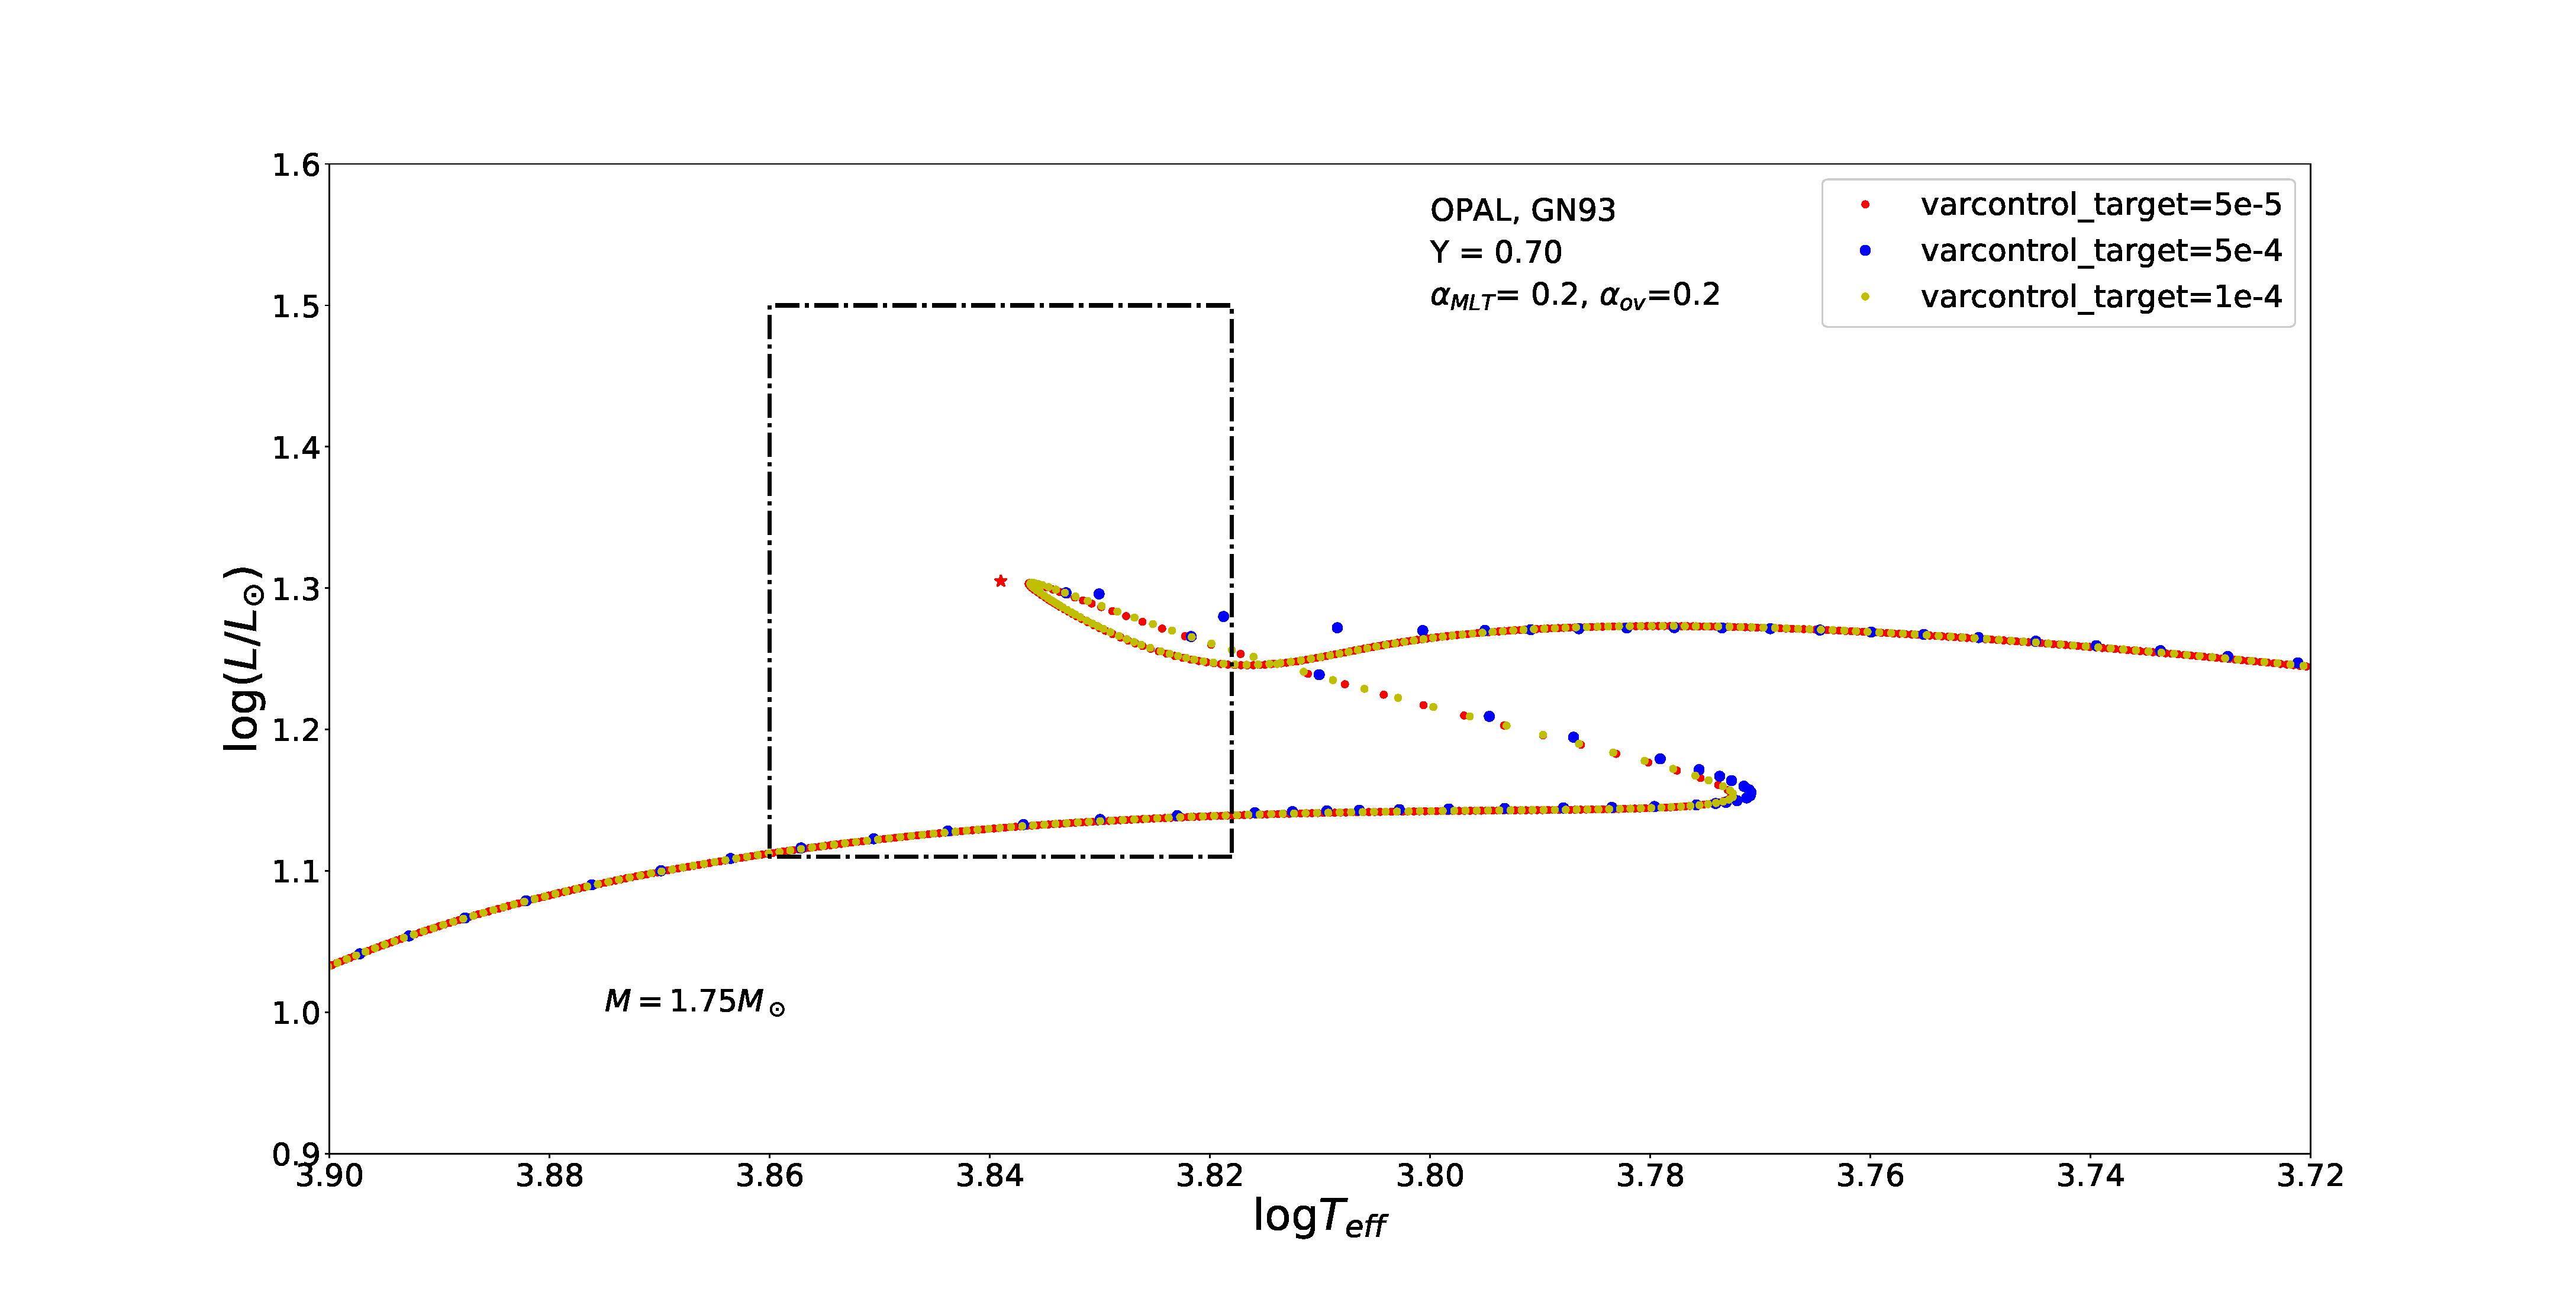
\includegraphics[width=1\textwidth]{varcontrol_res.eps}
	\makebox[\textwidth][c]{\includegraphics[width=1.2\textwidth]{frontpage.png}}%
\end{figure}
\newpage
\begin{abstract}
	
	The $\delta$ Sct stars 44 Tau and HD 187547 are investigated through asteroseismic modeling with the aim to determine their evolutionary stages. Several multisite campaigns have been carried out for 44 Tau, which led to successful modeling of the modes. HD 187547 has also been observed, resulting in an estimated large frequency separation of $\Delta\nu = 3.5d^{-1}$. This star has an unusual pulsation pattern  that is not yet understood. Modeling is needed in order to understand the processes in the star. 
	
	A grid of  $\sim$1000 tracks is constructed using the stellar structure and evolution code \texttt{MESA}. The pulsations along the tracks are calculated with the pulsation code \texttt{GYRE}. For all tracks, the observed frequencies, effective temperature, surface gravity, and luminosity are compared to the theoretically produced values. Two different runs are carried out for HD 187547, to investigate whether the estimate of the large frequency separation of $\Delta\nu = 3.5d^{-1}$ is potentially the double value $\Delta\nu=7d^{-1}$. 
	
	The results for 44 tau places it on the post-main sequence after hydrogen exhaustion. This is at a later stage than previous modeling has shown. However, the analysis conducted here has not taken mode identification into account and further investigation is needed to ensure that the frequencies are weighted correctly. For HD 187547 the results indicates that the star is a early to middle stage of the main sequence.  For $\Delta\nu = 3.5 d^{-1}$ the resulting best model is outside of the regime of $\delta$ Sct pulsations, contrary to the best model for $\Delta\nu = 7d^{-1}$. This suggests that the estimate of $3.5 d^{-1}$ is too low to agree with the low measured luminosity measurements by the GAIA mission, and that the star is younger than previously anticipated.  
	

\end{abstract}
\newpage
\chapter*{Acknowledgements}

First and foremost, I would like to express my sincere gratitude to the people who have helped me through my research, making this thesis possible. 
A very special thanks my co-supervisor Victoria Antoci, who not only opened my eyes to the exciting field of asteroseismology, but made the project entirely possible. She has guided me to become a better researcher, and this thesis is a product of that. 
Also a big thanks to my main supervisor Günter Houdek who helped me during the enormous task of grasping the concepts behind numerical simulations and the theory of stellar structure and evolution.  

I am also extremely grateful for the help provided by Earl Bellinger, without whom I would  probably still bee stuck in a forloop. His knowledge in computer science has helped me on countless occasions to  increase my coding skills.  Thanks to Kuldeep Verma and Jakob Lysgaard Rørsted for helping me understand the complicated mystery of the computational tools used in this project. To Rasmus Handberg for always being ready to help and discuss the best ways of implementing the \chis, and to Amalie Louise who always takes her time to help with anything that needs helping.  

This research would not have been carried out without the help of my office mates who have lend an ear to many frustrated hours of writing, coding and reattempting. Thanks to Simon Banerjee for always being ready to discuss problems, to Rasmus Lind Bjerre for putting a smile back onto my face when I was struggling and to Dorte Thrige Plauborg who has been my rock to lean on throughout the entire process. 
Finally, I wish to thank all my friends and my family for the support and understanding I have received. A heartfelt thanks to my boyfriend Emil Christensen who always kept understanding, supporting and loving me. 

\newpage
\tableofcontents
\chapter{Introduction}

The field of astronomy is one of the oldest sciences in the world, attempting to answer any question on the universe an the celestial bodies within it. Throughout the years it has developed into several theoretical and observational branches studying every corner of the universe from the nearest objects such as the moon an the Sun to the very edges of the universe that are so far away that the human brain cannot grasp the sheer size of it. Since the early studies to present day, astronomy has developed substantially, yet many questions remain still unanswered. What does the universe consist of? How old is the universe? Why are we able to exist here on Earth? Some of these may not be answered ever, yet curiosity drives humans to continue researching. 

One of the major components in the universe is the stars. New stars are born from the "ashes" of dead stars and learning how they are formed, evolve and die is fundamental for understanding the environment they evolve in. Such studies are within the field of \textit{Stellar Structure and Evolution}. Describing the different type of stars is an immense task in itself and dividing them into categories and understanding them requires us to understand the processed that leads to differences in their stellar structures. The problem with this is, however, that the insides of stars is unreachable from an observational point of view. We cannot simply look inside the stars, and for a long time penetrating the barriers of stellar layers seemed unobtainable.

Records on observations of pulsating stars goes back nearly 500 years. It was not until 1980's that we fully understood the potential of pulsations. At his point, the field of \textit{asteroseismology} was introduced by \citet{christensen1984} as    
\say{The science of using stellar oscillations for the study of the properties of stars, including their internal structure and dynamics}.

The closest (and therefore most studied) star is the Sun. Knowledge provided from the Sun can be projected to other types of stars, and \textit{helioseismology} (asteroseismology of the Sun) has provided valuable research in the field of Stellar Structure and Evolution. However, helioseismology is not yet developed enough to the reach the deepest layers of the Sun where the core recides. Therefore, we need to turn to other types of stars and exploit their pulsational advantages to reveil the secrets inside the stars. 

Before computers were invented, every observation and calculation were done analytically, which was a very time consuming task. Full stellar evolution tracks could simply ot be carried out. However, we are now at a time where stellar evolution can calculated fully numerically and results compared to the expected parameters derived from observations. Stellar structure and evolution codes can further provide calculations of the pulsations in a star with a stellar pulsation code. This is crucial for stellar modeling as the pulsation frequencies acts as an additional constraint to the parameter space. This constrain can help identify the processes inside pulsating stars, and thereby obtain knowledge on the pulsation mechanism, structure, convection, and evolutionary stage. 

In this work the method of asteroseismic modeling is applied to two different $\delta$ Sct stars, 44 Tau and 187547 (From here on referred to as Superstar). 44 Tau has already been modeled which to estimate the the evolutionary stage. By using a similar method in this work and comparing results, the procedure can be evaluated and adjusted to further be applied to Superstar. Asteroseismic modeling is particularly needed for this star since it represents some of the issues with the theory behind $\delta$ Sct stars. The goal of the asteroseismic modeling in this work is ultimately to analyze how well theory matches observations and using the results to discuss the remaining issues in the field and optimize the methods for any future work.  The work can be utilized on other types of stars, so a deeper understanding of stellar structure and evolution in general can be achieved. Hence, we get one step closer to understanding one of the most fundamental parts of the universe. 

 The work is structured as follows: \chapref{stellarstruc} gives an introduction to Stellar structure and evolution related to  this work. Relevant numerical results are presented to demonstrate key aspects of the field. \chapref{chap:asteroseismology} introduces the theory behind asteroseismology, and how it can be applied to various types of star, depending on the structure of the star. In \chapref{deltascuti} the $delta$ Sct stars described in more detail with the focus being on their importance from an asteroseismic and modeling point of view. Specifically, the asteroseismic and observational background of 44 Tau and Superstar are introduced. The tools used for modeling these star are presented in \chapref{compute}, where the Stellar Structure and Evolution code \texttt{MESA} and Stellar Pulsation code \texttt{GYRE} and their main numerical aspects are presented. \chapref{modeling} described the entire process of modeling the stars and the methods applied to compare to observations. Main results and proposed future work is then discussed in \secref{sec:discussion} and final conclusions are given in \chapref{sec:conclusion}.

This work has made use of data from the European Space Agency (ESA) mission
Gaia (\url{https://www.cosmos.esa.int/gaia}), processed by the Gaia Data Processing and Analysis Consortium (DPAC,
\url{https://www.cosmos.esa.int/web/gaia/dpac/consortium}). Funding for the DPAC
has been provided by national institutions, in particular the institutions
participating in the Gaia Multilateral Agreement.
\chapter{Stellar Structure and Evolution}
\label{stellarstruc}
The field of stellar structure and evolution is wide and it is possible to study numerous aspects of it. In this section, a brief introduction to the theory of stellar structure and evolution is given. This is based on mainly \citet{christensen2008lecture} and \citet{kippenhahn1990stellar}.   

It is difficult to paint a general picture of a "star". There are numerous types of stars, varying in observable properties such as magnitude and effective temperature, but also indirect properties such as their inner structures. Assumptions and simplifications are therefore necessary in order to  give a comprehensible  representation of a star. First, and foremost, a star is always assumed to be in \textit{hydrostatic equilibrium}, meaning that physics on a macroscopic level adapts to the surroundings on a timescale much faster than the \textit{free-fall time} (i.e. the time it takes until the interstellar cloud has contracted to a single point. The star is also assumed to have none or little rotation such that it can be treated as spherically symmetric. Magnetic fields are commonly assumed to not be present in the star. These assumption are of course very crude, as we know that stars do indeed rotate and have magnetic fields. However, the assumptions provides us the possibility to give a rough estimate on the conditions in a star. 

A star in hydrostatic equilibrium balances its own gravitation with the gas pressure. By looking at an infinitesimal small mass element $dm$ at a distance $r$ from the center, one can derive

\begin{equation}
    \frac{dP}{dr} = - \frac{GM(r)}{r^2}\rho
\end{equation}

\noindent where $G$ is the gravitational constant, $P$ is the pressure at a distance $r$ and $\rho$ is the density. This equation states that the pressure obtained from gas and radiation must be equal to that of gravitation in order to maintain hydrostatic equilibrium. A star is also assumed to follow the equation of mass-conservation 
\begin{equation}
    \frac{dM(r)}{dr}  = 4\pi r^2 \rho,
\end{equation}

\noindent where $M(r)$ is the mass of a spherical shell of  radius $r$. Combining the two equations yields

\begin{equation}
    -\frac{dP}{dM(r)} = \frac{G}{4\pi}\frac{M(r)}{r^4}.
    \end{equation}

\noindent From these equations it is possible to derive expressions for the minimum value of the central pressure $P_c$, the mean pressure $\Tilde{P}$ and temperature $\Tilde{T}$ for the case of a homogeneous star. Here, no knowledge on the composition is required, only the mass distribution.

The energy in a star is defined by the energy generation (and loss)  in a certain layer. The conservation of energy is then defined as

\begin{equation}
     \frac{dL}{dM(r)} = \epsilon = \epsilon_{nuc} - \epsilon_{\nu} - T\frac{\partial s}{\partial T},
\end{equation} 

\noindent where $\epsilon_{nuc}$ is nuclear energy generation rate, $\epsilon_{\nu}$ is the neutrino loss rate and $T\frac{\partial s}{\partial T}$ is the gravitational energy rate describing energy that is released or absorbed by the contraction or expansion of the star. The energy can be transported through radiation. The temperature gradient required to carry the entire luminosity of a star by radiation can be written as 

\begin{equation}
\label{transportradiative}
	\frac{dT}{dr} = -\frac{3 \rho}{64\pi^2 \sigma }\frac{\kappa L}{r^4 T^3},
\end{equation}

\noindent also called the equation of radiative transport. Here $L$ is the luminosity, $\kappa$ is the opacity, $\rho$ is the density and $\sigma$ is the Stefan-Boltzmann constant. This equation is valid as long a the \textit{diffusion approximation} is valid. This breaks down at the stellar surface of the star when the gas becomes optically thin. In this case the full, and much more complicated, equations of radiative transfer must be solved.

For a more thorough description of stellar structure, the properties of the matter need to be assessed. Describing the thermodynamical properties in detail is no simple task, but the fundamental assumption is that at any point in the star, the gas is assumed to be in \textit{thermodynamic equilibrium}, which means that there are no net macroscopic flows. This approximation ensures that instead of considering detailed reactions between particles, the average properties of the gas can be described by local state variables. The relations between these specifies the \textit{equation of state} (EOS) of the gas. It is also assumed that there is no change in the gas conditions over the distance of the mean-free-path of a particle located in the gas, or over the time between collisions. These assumptions are well applied in stellar interiors, but in order to describe conditions in the atmosphere, a more detailed description is needed. 

Since temperatures in the interiors are high, most of the gas will be fully ionized, and thereby have no internal degrees of freedom. Interactions b (collisions) between particles can be neglected, hence the gas is an approximate \textit{ideal gas} following the ideal-gas law

\begin{equation}
    PV = N k_B T,
\end{equation}

\noindent where $N$ is the number of particles in a gas with volume $V$, and $k_B$ is Boltzmann's constant. From this, general relations between pressure and internal energy can be derived. Stellar structure and evolution solves both equations of hydrostatic equilibrium and the EOS of the star. The modules used in this project will be described in \chapref{compute}. 


\section{Energy transport by convection}
\label{sec:energybyconvection}
When deriving the equations and variables for a star, it is usually assumed that the star can be treated as being spherically symmetric. In reality though, there will be fluctuations on small scales that has to be taken into account. The most considered of these instabilities or fluctuations is \textit{convection}. These can be treated as small perturbations. 

Convection can be described as macroscopic mass elements or "bubbles" that transports energy in a star. Elements that are hotter than their surroundings rises upwards carrying excess thermal energy. The displacement of the element grows exponentially and when the velocity becomes too large, nonlinear effects causes the thermal energy to be released into the surroundings. Thus, convection contributes by transporting energy, and mixing the gas elements. This has large consequences for the stellar evolution as we shall see in \secref{compute}. 

Whether a region in a star is stable against convection depends on whether the perturbation is allowed to grow under certain conditions. Therefore, it is a matter of \textit{convective instability}. Assuming that the mass elements do not exchange energy with the surroundings (during movement), and therefore moves adiabatically, it can be derived that 

\begin{equation}
\label{instability_eq}
    \nabla < \nabla_e + \frac{\phi}{\delta}\nabla_{\mu},
\end{equation}

\noindent describing the condition for convective stability. Here

\begin{equation}
    \nabla \equiv \left(\frac{d \ln T}{d \ln P}\right)_s, \qquad \nabla_e \equiv \left(\frac{\partial \ln T}{\partial \ln P}\right)_e, \qquad \nabla_\mu \equiv \left(\frac{\partial \ln \mu}{\partial \ln P}\right)_s.
\end{equation}

\noindent Here, the subscript $e$ means that the derivative is in relation to the element, whereas $s$ is the surrounding material. %Both $\nabla$ and $\nabla_\mu$, the derivatives are spatial with depth measured in P, whereas $\nabla_e$ varies T with the depth position of the element itself.
For the case where energy is transported by radiation or conduction only

\begin{equation}
    \nabla_{rad} \equiv \left(\frac{d \ln T}{d \ln P}\right)_{rad}, 
\end{equation}

\noindent temperature variation is described with depth. In a layer where all energy transport is either radiation or conduction, $\nabla = \nabla_{rad}$. Also, assuming that the element moves adiabatically such that 

\begin{equation}
\label{stability}
    \nabla_e = \nabla_{ad} \equiv \left(\frac{\partial \ln T}{\partial \ln P}\right)_{ad}
\end{equation}

\noindent and inserting in \eqref{instability_eq}, one arrives at

\begin{equation}
\label{stability2}
    \nabla_{rad} < \nabla_{ad} + \frac{\phi}{\delta} \nabla_\mu,
\end{equation}

known as the \textit{Ledoux criterion}. Under the assumptions mentioned earlier, this is the criteria for dynamical stability. It can be simplified further by assuming that the chemical composition is homogeneous such that $\mu$ is constant. This yields the \textit{Schwarzschild criterion} on the simple form:

\begin{equation}
\label{stability3}
    \nabla_{rad} < \nabla_{ad}.
\end{equation}

\noindent This assumption does not apply well to evolved stars where elements are not necessarily produced in  the same layer (as heavier elements are produced below lighter). 
Instability to convection thus occurs when the left hand side becomes larger than the right hand side. The small perturbations will grow until the layers is filled with convection. This occurs if

\begin{itemize}
    \item $L(r)/m(r)$, (the energy generation rate per unit mass within radius $r$) is large. In massive stars, this rate is an increasing function of temperature, thus increasing $L/m$ towards the center. Therefore these stars have convective cores.
    \item $\rho/T$ is large. Since $\rho/T^3$ increases rapidly in the photosphere, this usually occurs in cooler stars. 
    \item The opacity $\kappa$ is large. Stars with low surface temperatures usually have higher $\kappa$ in the outer layers. 
    \item $\nabla_{ad}$ is small. This happens in ionization zones.
\end{itemize}

To sum up, the first condition consequently allows for convection in the core of massive stars. The remaining conditions for outer layers of cooler stars. The different possibilities for the structures are illustrated on \figref{convectionzones}. 

\begin{figure}[htbp]
    \centering
    \includegraphics[width=1\textwidth]{convection_zones.png}
    \caption{Estimated occurrence of convection zones in main-sequence stars with different masses. Stars with masses higher than ~2 \msun have fully convective cores and only a very thin convective shell. Less massive stars with masses below 1\msun have deep convective envelopes. The stars in between marks the transition between the two. They have convective cores and a thin convective outer layer.}
    \label{convectionzones}
\end{figure}

The stars in this project lies in the \textit{intermediate mass} range which is usually stars of masses between 1.5\msun and 2.2\msun. They cover the transition from deep convective envelopes and convective cores. The motivation for using such stars will be discussed further in \secref{sec:why}.

If \eqref{stability2} leads to stability it follows that $\nabla = \nabla_{rad}$ for the entire layer. The  last possibility is that one of \eqref{stability2} and \eqref{stability3} says stability whereas the other says instability, see \citep{kippenhahn1990stellar} for more details.
 
This prescription gives a very simplified picture of where convection is expected to occur within a star. However, in reality a local treatment is complicated since convective motion is not only dependent on local forces, but forces between layers as well (such as momentum and inertia). The border of a convective zone is thereby not well-defined and precise as elements accelerated from one layer might flow into another. This will be discussed further in \secref{sec:conv_prescriptions}. 
Convection flows in the laboratory is relatively well described by reasonable approximations. However, in stars convection is happening in much more violent conditions where compression of gas and turbulent motion depends on density, pressure and gravity of very high orders.  Taking such effects into consideration is not simple by any means, but efforts have been made to implement convection by making full two- and three-dimensional hydro dynamical simulations (e.g. \citet{nordlund19903}). Such codes do not treat the convection as separate homogeneous bubbles, but as a fully coupled time-dependent system. Such codes give a much more detailed and realistic picture of convection for single models. However, since the computation time for the full convective solution of a model is much longer than a simplified version, calculating a full track is not yet feasible. Therefore, the most used method is the \textit{standard mixing length theory} \citep{weiss2004cox}, which is a time-independent assessment. This is not sufficient to describe full hydrodynamical convection, but allows approximations to give a simplified local treatment, where convection can be described as macroscopic mass elements transferring energy. The mean free path is described with \textit{the mixing length}. There are several ways to implement this in stellar modeling which will be described in \secref{sec:conv_prescriptions}. 


\section[Stellar evolution through the HR-diagram]{Numerical results for stellar evolution through the HR-diagram}
This section describes the evolution of a star through numerically calculated stellar evolutionary tracks, mainly focusing on the main sequence (ms)) and immediate post-main sequence (pms) phases of intermediate mass stars

Stars are born from molecular clouds, collapsing under their own gravity. When the cloud reaches a the \textit{Jeans Mass}, the \textit{Jeans Criterion} is fulfilled, meaning that any perturbation will cause a free-fall collapse. This continues while the process happens isothermally until the free-fall time becomes similar to the timescale for thermal adjustment. The process then becomes adiabatic, stopping the rapid dynamical contraction and leaving behind a \textit{protostar} in hydrostatic equilibrium. Due to their low internal temperature and high opacity, these stars are fully convective. Thereby they are born on the \textit{Hayashi Track} where the contraction continues. This track is the beginning of the \textit{pre- main sequence phase}. As the star contracts and descends on the Hayashi track, the surface temperature (or effective temperature) is essentially constant while the luminosity decreases. The star heats up from the inside out since gas escapes the outer layers more easily. As the center becomes hotter, the opacity decreases and the convection zone slowly recedes. The star then leaves the Hayashi track and proceeds a radiative contraction on \textit{the Henyey track}. This causes the decreasing luminosity trend to reverse and the star becomes more luminous. Eventually the core temperatures will be sufficiently high to trigger the proton-proton reaction, converting H into deuterium ($^{2}\text{H}$) and thereafter $^3\text{He}$.\footnote{The full proton-proton chain is not yet completed since the temperature is still too low to burn hydrogen in full equilibrium.} 

%!!!Something happens here, understand it (Aearts p. 35)

As a result, a convective core is created. This will however disappear if the mass of the star is below 1.1\msun, whereas stars of higher mass will burn hydrogen in the cores through the \textit{CNO-cycle}. Accretion of mass continues on the PMS phase on a thermal timescale. Stars of masses larger than 9\msun moves so quickly into the MS phase that they are unobservable on the PMS due to the thick shell of accreting mass, while stars of masses between 1.6-9\msun end their accretion of mass on the PMS. When the star begins burning hydrogen in full hydrostatic equilibrium it is born onto the \textit{zero-age main-sequence} (ZAMS). Stars below 0.08\msun never reaches ZAMS because their internal central temperature never becomes high enough to fuse hydrogen to helium in equilibrium. Instead they become degenerate, and are known as \textit{brown dwarfs}. Although stellar pulsations in brown dwarfs were theoretically predicted by \citet{palla2005pulsating} these pulsations have not yet been detected \citep{aerts2010, cody2014pulsation}. 

The ZAMS is where the star begins the life on the main-sequence where it spends 90 \% of its life burning H to He. The computed solutions from this stage on can be seen on \figref{stages}. The main sequence corresponding to the hydrogen burning in the core is defined as the phase between point 1 and 2. For all stars, the luminosity increases during this phase. The reason for this is that the hydrogen is converted into helium which causes the mean molecular weight to increase, which can be seen from

\begin{equation}
\label{meanmol}
\mu \simeq \frac{4}{3+5\text{X}-\text{Z}},
\end{equation}


\noindent where X, Y and Z is the hydrogen, helium and metal fraction respectively. It follows from the ideal gas law that $P \propto \rho T$. The pressure must balance the weight of the overlaying layers, hence it cannot decrease. Instead, $\rho T$ compensates for the increase in $\mu$. The core will start contracting to increase $\rho$ and gravitational potential energy energy is released, which further causes an increase in T (from the Virial theorem\footnote{See Chapter 3 in \citet{kippenhahn1990stellar}}. As the opacity follows $\kappa \propto \text{T}^{-3.5}$, an increase in temperature will cause a decrease in opacity. Thus, the photons can escape more easily, and the luminosity increases. This also follows from the equation of radiative transport \eqref{transportradiative} where $L\propto 1/\kappa$.

It is more complicated to explain the change in global parameters such as the effective temperature and radius. The radius increases in general as the star evolves, but the rate of this expansion is mass dependent. For stars that have low masses (close to 1\msun ) expansion is slow and the increase in luminosity will lead to an increase in the effective temperature as well, while it is the opposite for stars with higher masses and higher expansion rates. Since the star heats from the inside, the outer layers will have expanded before the temperature can increase in this region, hence the effective temperature decreases. 

%When hydrogen is exhausted in the core (point 2 on \figref{iben}) the star is left with a core consisting of helium. At this point the temperature in the core is too low to initiate helium burning, and the core is near isothermal. However, it is surrounded by a region where temperature is still high enough to burn hydrogen. This is called a \textit{shell source}. This provides the core with additional helium, hence increasing the mass causing it to contract and increasing the temperature until  
When hydrogen abundance get sufficiently low in the core, the star reaches the \textit{terminal-age main-sequence} (TAMS). Here, the core now consists of helium.
For intermediate mass stars,a noticeable feature is the "hook" following the ms, also known as the \textit{Henyey Hook} (not to be confused with the Henyey track). This is clearly depicted on \figref{stages2} As these type of stars have convective cores, the energy production will decrease uniformly throughout the core. The star will attempt to compensate for this by increasing the central temperature and keep the energy production up, hence causing the core to contract. As a result of the contraction, gravitational potential energy is released, where half is converted to thermal energy, heating up the core and essentially shifting the evolution to higher effective temperatures. This phase is in the order of a few megayears, which is extremely fast evolution compared to the main sequence (in the order of $10^{10}$ yrs. Therefore, studying a star in this exact phase is very difficult since a star can only be verified to be in this phase through modeling, as observations in color-magnitude diagrams cannot resolve it. From now on this will be referred to as the \textit{post main-sequence contraction phase}. At this point most of the energy production still comes from nuclear reactions, and the gravitational contribution is small in comparison.  It is surrounded by a region where temperature is still high enough to burn hydrogen, and slowly establishes a \textit{shell source}. This will however not be dominant until all hydrogen is exhausted. When this happens at point 3 on \figref{stages}, the evolution is accelerated and the star is no longer in thermal equilibrium. The contracting core will thus be accompanied by an expanding envelope, causing the effective temperature to decrease. This phase will be referred to as the \textit{post- main sequence expansion phase}. The outer convection zone deepens until is reaches the layers where nuclear fusion has occurred (the core). This is marked as point 5 and is also called \textit{first dredge up}. 

\begin{figure}[htbp]
    \centering
    \includegraphics[width=0.8\textwidth,angle=-1]{iben.png}
    \caption{\citep{kippenhahn1990stellar} Stellar evolution tracks of masses ranging from 0.25\msun to 15\msun. The numbers indicate different stages in the evolution. Figure from \citet{iben1967stellar}.}
    \label{stages}
\end{figure}

\begin{figure}[htbp]
	\centering
	\includegraphics[width=0.8\textwidth]{STAGES.png}
	\caption{\citep{kippenhahn1990stellar} Stellar evolution track of a 5\msun star. The main sequence is marked between A and B, the post-MS contraction from B to C and the post -MS expansion is after C. Figure from \citep{kippenhahn1990stellar}.}
	\label{stages2}
\end{figure}

%As a consequence of this contraction, the conditions in the core become violent enough to ignite helium. 
At point 5-6 , the star will then move back up the Hyashi track as a red giant. The further evolution from then is largely depending on the mass. Stars with masses between 0.5<M<2.3\msun (relevant for this work) will have a degenerate helium core by the end of the main sequence (the exact cutoff depends on the initial metallicity in the star). The core contraction following the main-sequence continues until it reaches a temperature high enough to ignite helium in the core through the triple $\alpha$ process.   A thermal runaway known as \textit{helium-flash} occurs and lifts the degeneracy of the helium core, settling the star down on the \textit{horizontal branch} where it burns helium in the core and hydrogen in a shell (for stars with M<2.0\msun). 
 Stars with masses below 4-8\msun finish nuclear burning  at carbon or oxygen. By the end, their envelopes will be ejected into space through stellar winds, forming planetary nebulae. Left behind is the remnant, a white dwarf star.
  %The further evolution to this stage will not be discussed further in this work, but refer instead to \citet{kippenhahn1990stellar, christensen2008lecture} and \citet{weiss2004cox} for more details.   

It has been shown how a star's luminosity changes as a function of effective temperature throughout its evolution. As mentioned in the beginning of the chapter, assumptions on hydrostatic equilibrium and equation of state can provide us with solutions that relates several other properties. The numerical solutions to the radius $R$,  surface gravity  $g$, core density $\rho$ and convective core mass are shown on \figref{stellarparams} as a function of time. The red vertical lines from left to right indicate the beginning of the MS, post-MS contraction and post-MS expansion phases. As for the radius, the star contracts for the entirety of the PMS. As it burns hydrogen on the MS it slowly expands (as the temperature in the core increases slightly with time) until the post-MS where it again contracts. After hydrogen exhaustion the star undergoes fast overall expansion. Another parameter which is highly relevant for the frequencies is the surface gravity, as we shall see in \secref{chap:asteroseismology}. From theory we know that $g \propto M/R^2$, which is equivalent to the numerical results shown on \figref{stellarparams}. The density in the center increases rapidly on the Hyashi track when the star contracts, and follows the linear tendency $\rho_c \propto \frac{3M}{\pi R^3}$ on the MS (by assuming $\rho$ is a linear function of the fractional radius $r$. At the immediate post-MS phase it increases again as the core contracts rapidly. 

An important parameter to also look at is the mass of the convective core. On the Hyashi track, the star is fully convective as it contracts. As the star burns hydrogen, the convective core mass slowly decreases until the point where hydrogen is exhausted in the core.  On \figref{convcore}, numerical results for the convective core mass ratio to the total stellar mass is plotted as a function of stellar age in Gyrs for tracks with different masses. It can here be seen that higher stellar masses leads to higher convective core masses. Since stars with higher mass also have shorter lifetimes on the MS, which is also well-depicted on the figure as the convective core mass drops to zero when nuclear fusion in the core ends, which occurs sooner for higher masses. At this point, the core will not longer have high enough temperature to be convective. The smaller inset window on \figref{convcore} shows the convective core mass evolution on the PMS to the MS. Higher masses enter the hyashi track at a lower age than stars with smaller masses again indicating a faster evolution in general.  
%\begin{itemize}
 %   \item log g / age 
 %   \item log R / log g
 %   \item density / Radius
  %  \item log R / age
%    \item P / age
 %   \item P / R
%\end{itemize}

\begin{figure}[htbp]
    \centering
   \makebox[\textwidth][c]{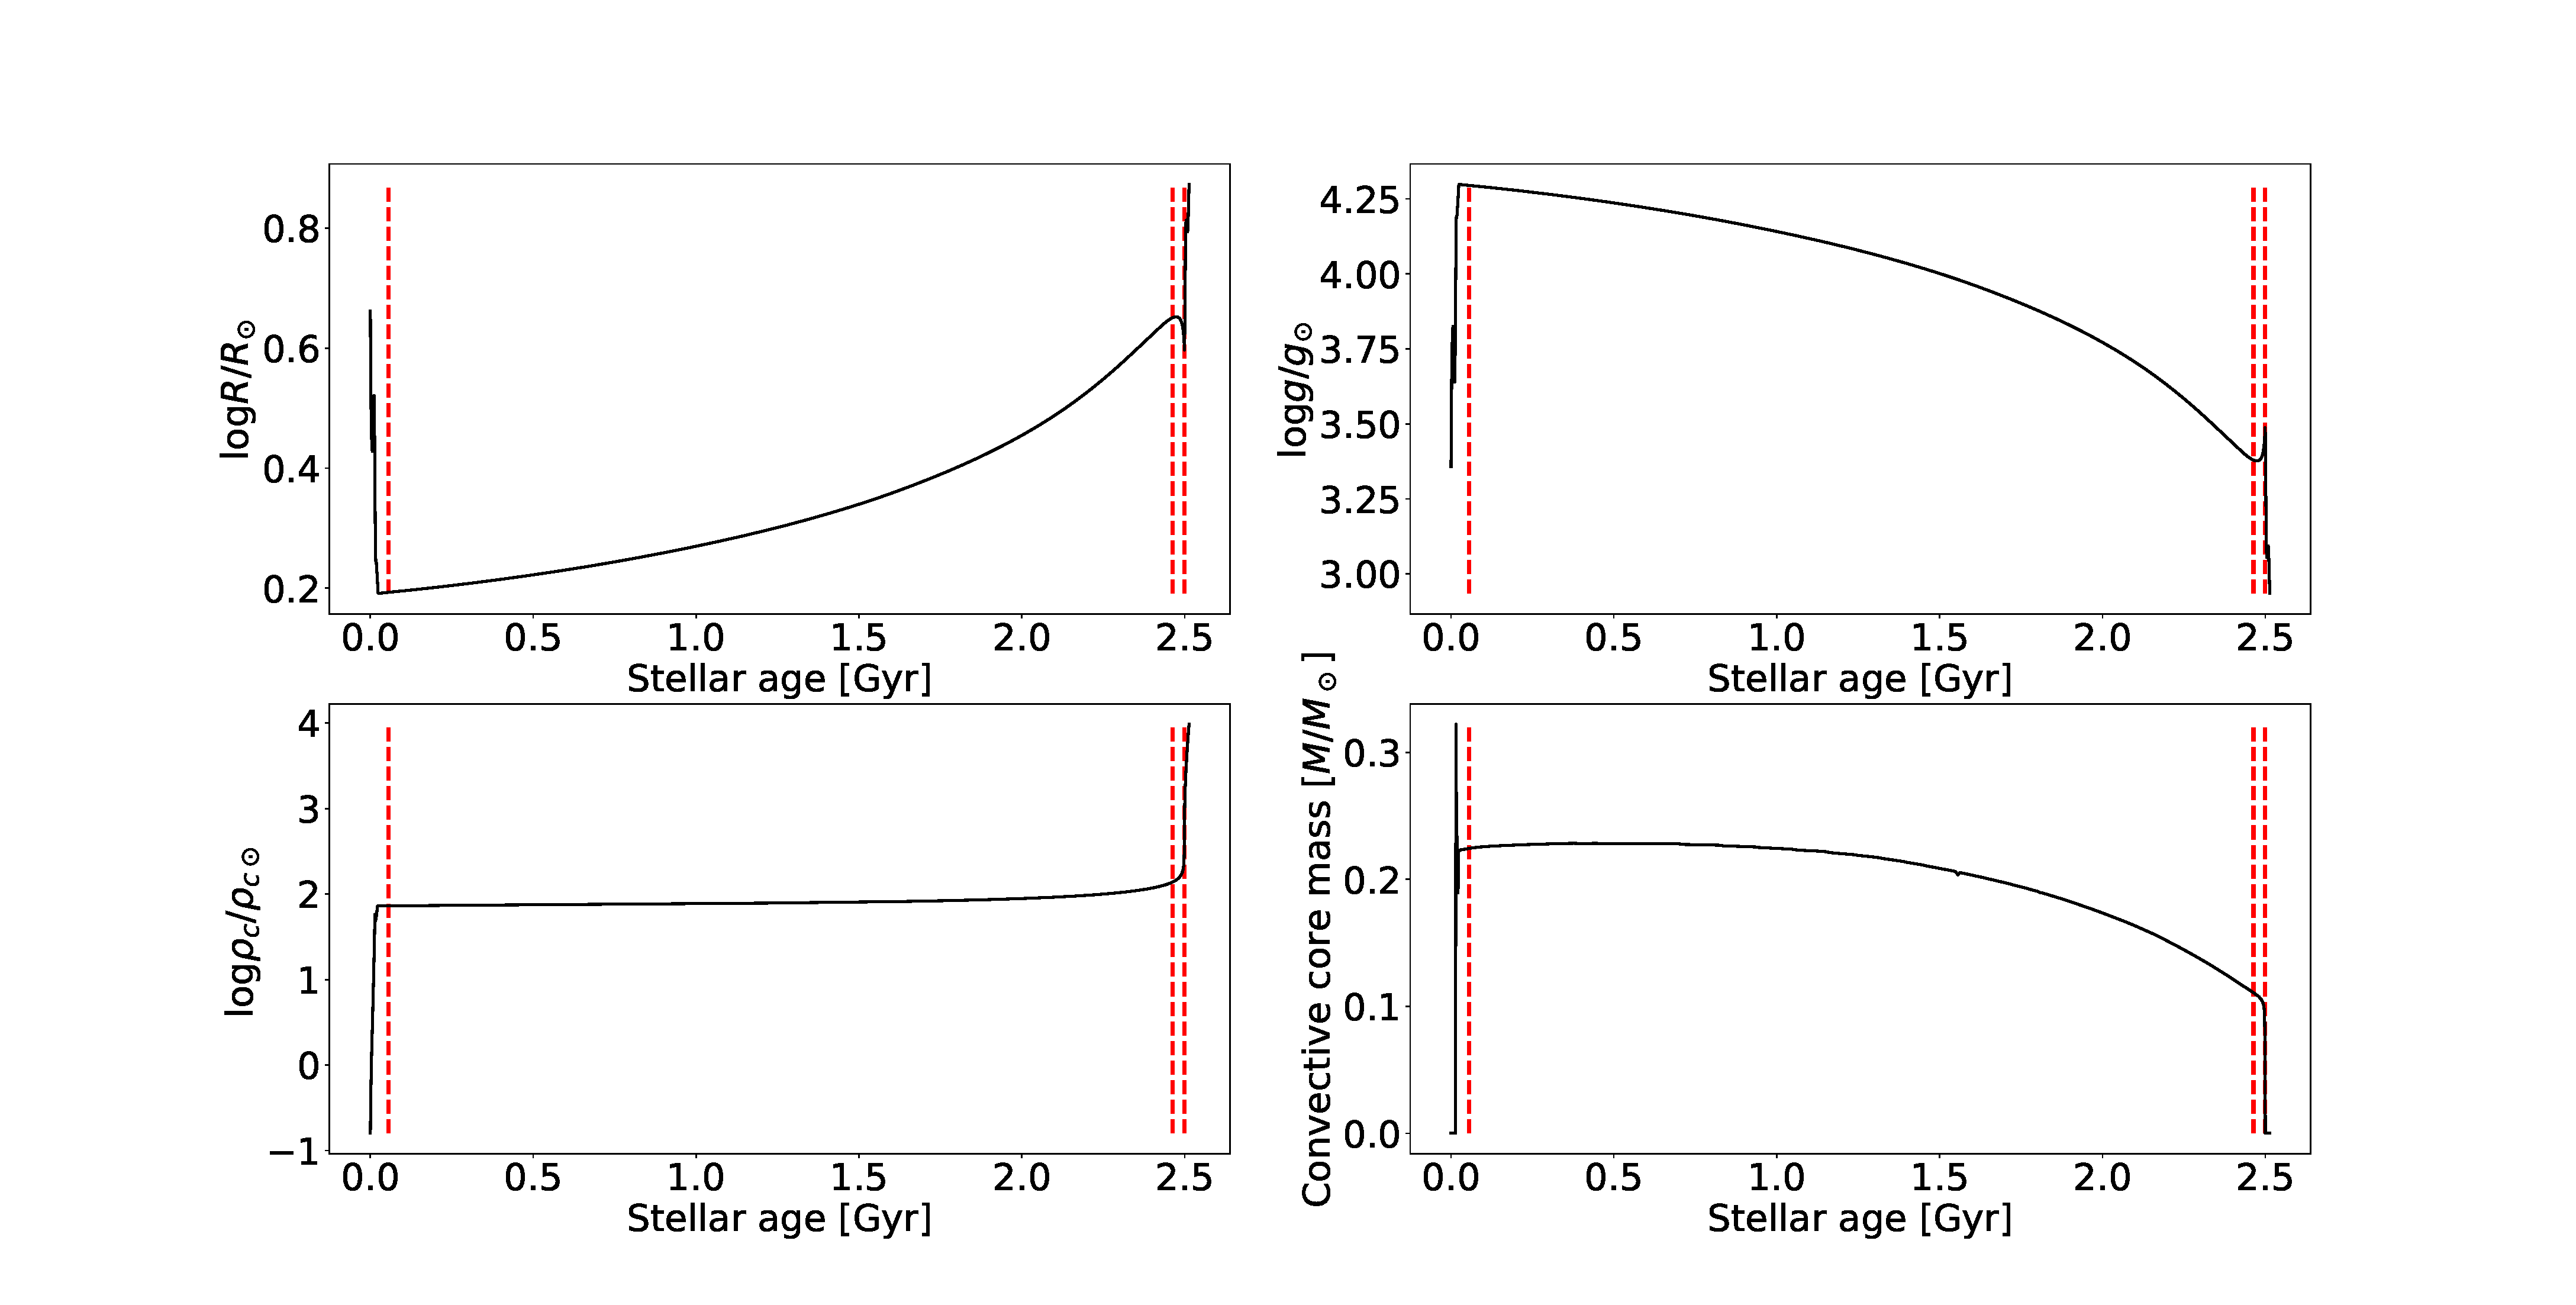
\includegraphics[width=1.2\textwidth]{stellarparams.eps}}%
    \caption{Numerically calculated stellar parameters for a track with 1.75\msun, X=0.75, Z=0.02, $\alpha_{mlt}$=0.5, $\alpha_{ov}$=0.3. The dashed lines marks the different stages of the evolution, leftmost being thew beginning of the main-sequence, middle one the post- MS contraction phase and rightmost the post-MS expansion phase.}
    \label{stellarparams}
\end{figure}


\begin{figure}[htbp]
    \centering
    \makebox[\textwidth][c]{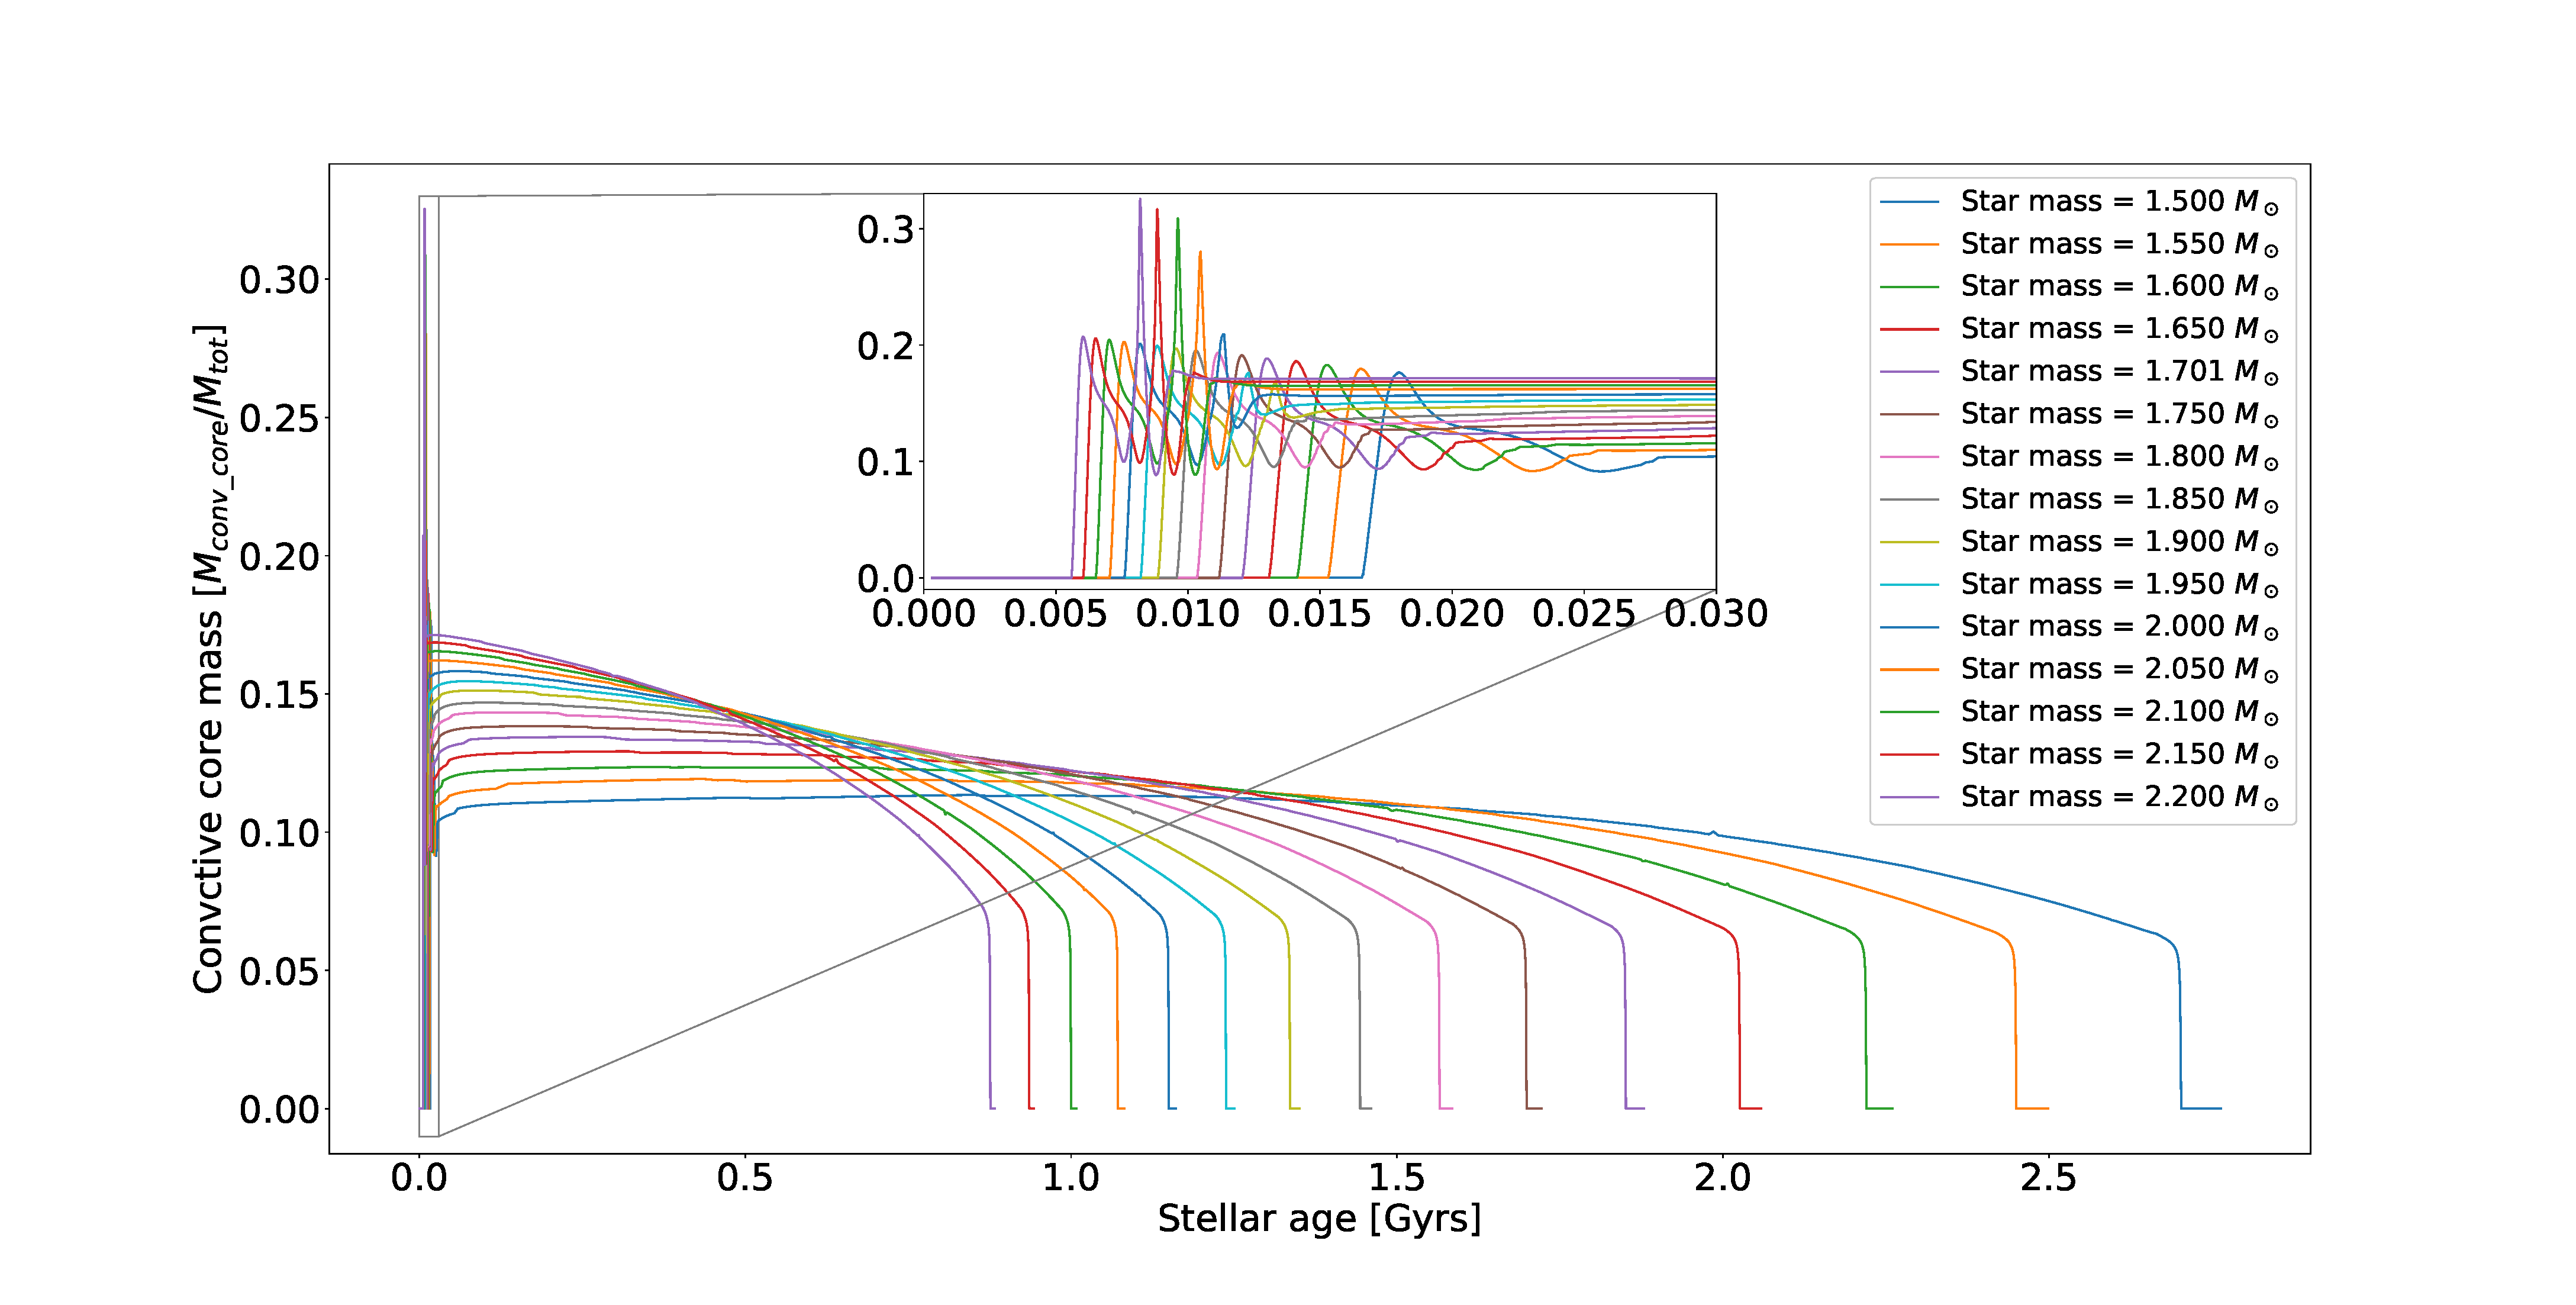
\includegraphics[width=1.2\textwidth]{conv_cores.eps}}%
    %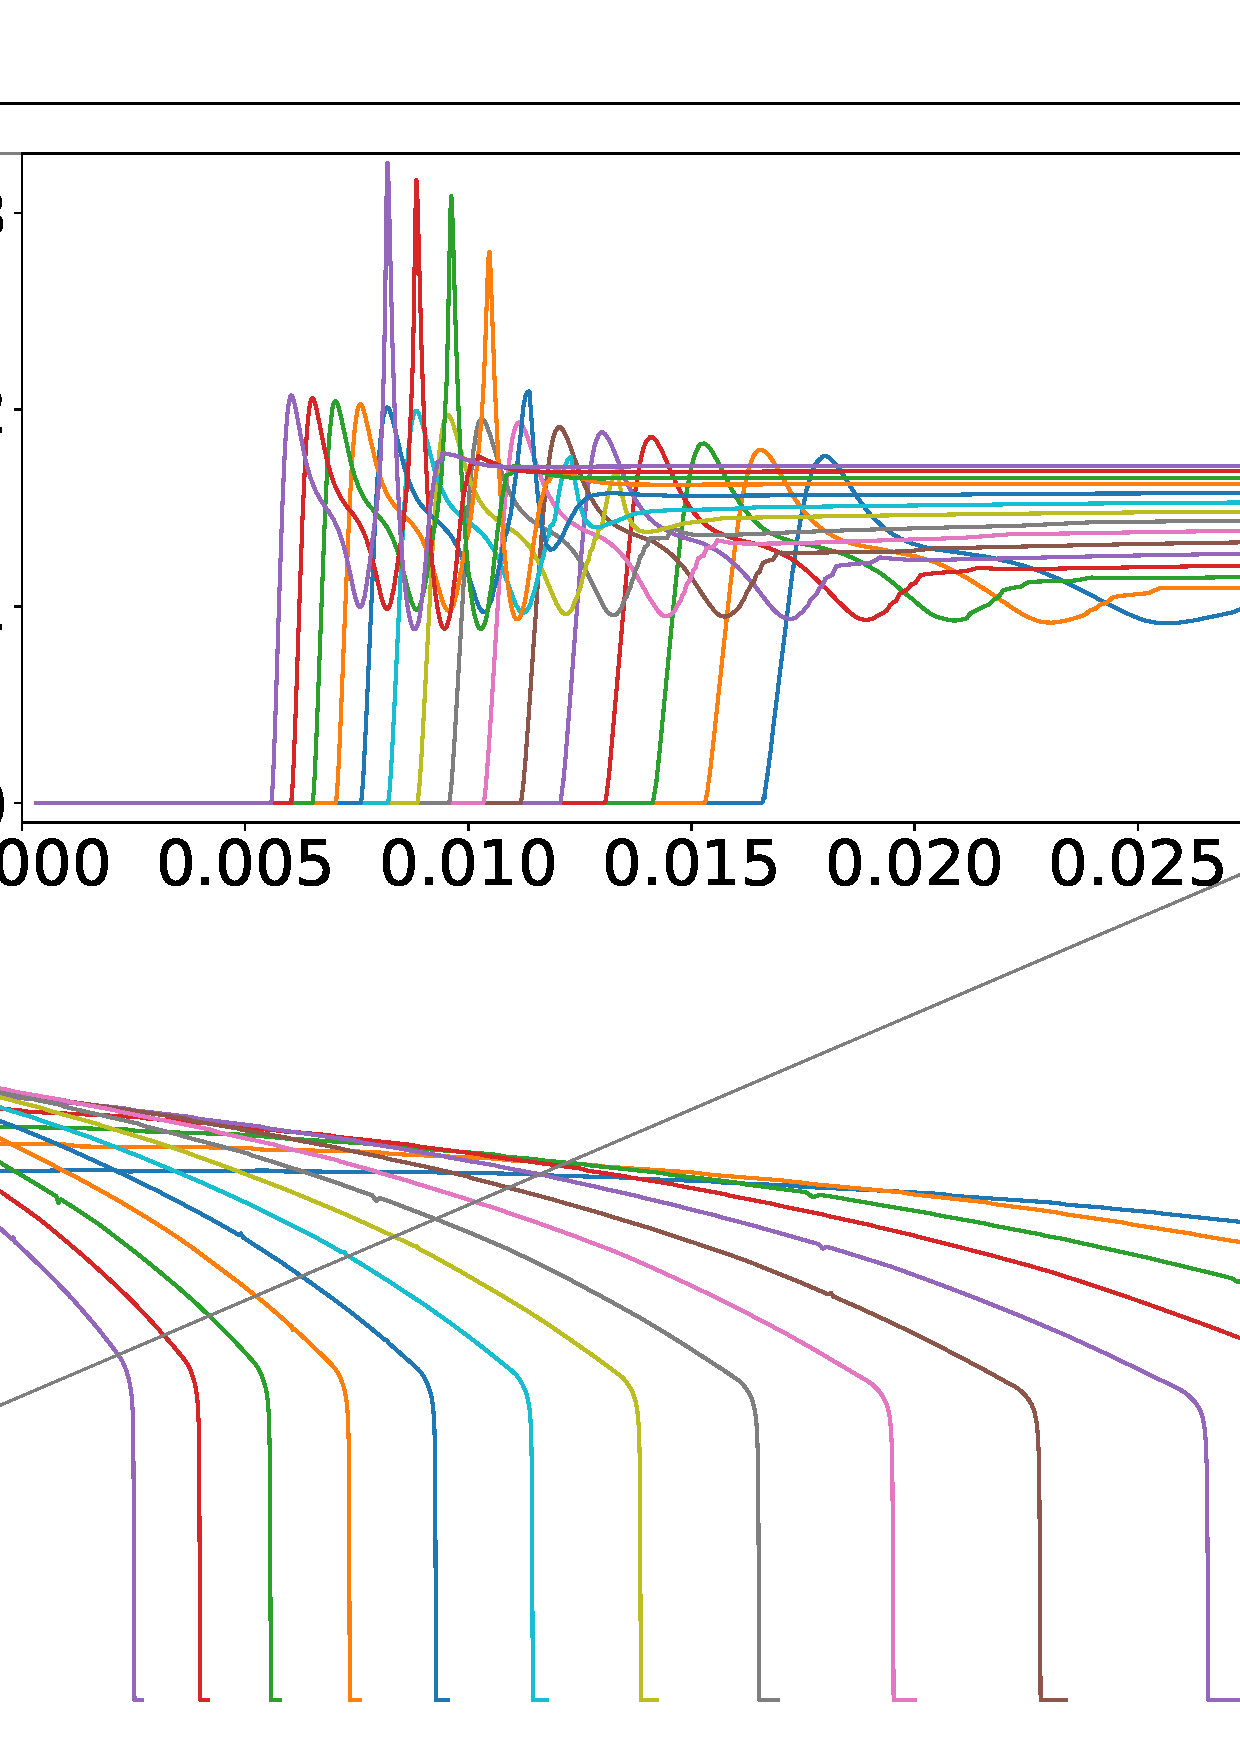
\includegraphics[width=1\textwidth]{conv_cores.png}
    \caption{Numerical results for stars with masses ranging from 1.5\msun to 2.2\msun, X = 0.70, Z = 0.02, $\alpha_{mlt} = 0.5$ and $\alpha_{ov} = 0.3$. The convective core mass ratio is plotted as a function of stellar age. The small window shows a zoom in of the plot at the age where the convective core is established (on the MS)}
    \label{convcore}
\end{figure}

%Regions of convective instability is determined from the instability condition which can be derived from the ideal gas law:

%\begin{equation}
%    \nabla \equiv \frac{d \ln T}{d \ln p} > %\nabla_{ad} + \nabla_{\nu},
%\end{equation}

%\noindent where

%\begin{equation}
 %   \nabla_{ad} = \left(\frac{\partial \ln %T}{\partial \ln p}\right)_{ad},  \nabla_{\mu} = \frac{d \ln \mu }{d \ln p}.
%\end{equation}

%Here, T is the temperature, p is the pressure and $\mu$ is the mean molecular weight.  
\chapter{An introduction to asteroseismology}
\label{chap:asteroseismology}

All stars are different in temperature, radius, luminosity, density and mass. Some stars also have \textit{pulsations}, meaning that their luminosities vary in certain periods. The field of asteroseismology exploits these stellar pulsations in a star to look inside it and determine the inner structure. There are several types of pulsations depending on particularly the mass. In this chapter, a brief introduction to key aspects in the theory of stellar pulsations are given.
 %takes advantage of the pulsations in a star. All stars are different in structure, temperature, radius, luminosity, density and evolution. This is also what separates them from each other in a stellar oscillation spectrum, since it is unique to each type of pulsating star. Some stars oscillates on the pre- ms, others on the ms, and some on the Red Giant Branch. The nature of the oscillation spectra thus allows us to distinguish between stars with different interiors.  
 
Pulsating stars contract and expands periodically, causing brightness changes that can be observed using two methods. Periodic brightness and thereby temperature variations causes variations in luminosity which can be measured with photometry. Changes in the velocity fields due to periodic changes in the luminosity gives rise to an observable Doppler effect which can be measured using spectroscopy. The outcome of the observations are time-series that can be converted to oscillation spectra through a fourier transform. The oscillation spectra can be analyzed to identify the nature of each frequency. Modeling the star can then reproduce the environment in the star, specifically the sound speed which changes according to the temperature and chemical composition. Therefore, comparing these theoretically produced frequencies with observations allows us to estimate the properties of the star.  

\section{Stellar pulsations}

Pulsations in stars are treated three-dimensionally, and usually assumes a spherical symmetry of the star (which is true when rotation of the star is so small that the distortion of the stellar symmetry is negligible and the spherical harmonics still apply, see \eqref{spherical}). The three directions for which the natural oscillation modes have nodes are described by the distance to the center of the star, $r$, co-latitude $\theta$ (measured from pulsation pole) and longitude $\phi$. Nodes are defined as concentric shells of constant r, cones of constant $\theta$ and finally planes of constant $\theta$. We can then describe the displacement in the ($r$,$\theta$,$\phi$) space as the following

\begin{align}
    & \xi_r(r,\theta,\phi,t) = a(r)Y^{m}_l(\theta,\phi)e^{-i2\pi\nu t}  \\
    & \xi_\Theta(r,\theta,\phi,t) = b(r)\frac{\partial Y^{m}_l(\theta,\phi)}{\partial \theta}e^{-i2\pi\nu t}  \\
    & \xi_\Theta(r,\theta,\phi,t) = \frac{b(r)}{\sin(\theta)}\frac{\partial Y^{m}_l(\theta,\phi)}{\partial \phi}e^{-i2\pi\nu t},
\end{align}

\noindent where $a(r)$ and $b(r)$ are the amplitudes, $\nu$ is the oscillation frequency (1/Period) and $Y^{m}_l(\theta,\phi)$ are the spherical harmonics given by 

\begin{equation}
\label{spherical}
    Y^{m}_l(\theta,\phi) = (-1)^{m}\sqrt{\frac{2l+1}{4\pi}\frac{(l-m)!}{(l+m)!}}P^{m}_l(\cos(\theta))e^{im\phi},
\end{equation}

\noindent where $P^{m}_l(\cos(\theta))$ are the Legendre polynomials\footnote{see \citet{aerts2010} for more details.}, with $l$ being the spherical degree and $m$ the azimuthal order \footnotetext{These equations are introduced for the sole purpose of presenting the spherical harmonics. They will not be used for calculations during the project. For more details, see \citep{aerts2010}.}. The normalization constant 
\begin{equation}
    c_{lm} \equiv \sqrt{\frac{2l+1}{4\pi}\frac{(l-m)!}{(l+m)!}},
\end{equation}

\noindent is defined such that the integral over the unit sphere of $|Y^{m}_l|^2 = 1 $. Three quantum numbers describes the modes for 3-D stars, $n$,$l$ and $m$. $n$ is the \textit{radial order} describing the number of radial nodes in the star. $l$ is the \textit{spherical degree} and represents the total number of surface nodes; finally $m$ is the \textit{azimuthal order} where $|m|$ is the number of longitudinal nodes, crossing the equator. It then follows that $l$-$|m|$ are the co-latitudinal nodes. $m$ can vary from $-l$ to $l$, yielding therefore a number of $2l+1$ different nodes for each spherical degree. An example of all geometrical possibilities of an $l=3$ mode can be seen on \figref{l3}. 

\begin{figure}[t]
    \centering
    \includegraphics[width=0.8\textwidth]{nonradial.png}
    \caption{Possible geometrical nonradial pulsation patterns with $l$=3 for a spherically symmetric star. The '+' indicates areas that moves towards the observer, and the '-' away from the observer. \citep{antoci2011excitation} (adapted from Wolfgang Zima 1999 master thesis.)}
    \label{l3}
\end{figure}

Generally we can divide stellar pulsations into radial and non-radial pulsations. Radial pulsations is the case for which $l=0$, with the very simplest geometry being the $n=1$ or \textit{radial fundamental mode}. In this case there is a node only at the center with the corresponding anti-node at the surface, meaning that the entire star pulsates. $n=2$ is the first radial overtone with one node, $n=3$ the second overtone has two radial nodes and so on. %The cases for the radial modes can be seen on \figref{radial}.
If we assume that the star is uniform in temperature and chemical composition we would expect the ratio between the fundamental mode and the first overtone to be similar to that of an organ pipe \citep{aerts2010}. However, since we know that the temperature and chemical composition in the star changes with radius, we can exploit the fact that the sound speed changes accordingly, hence affecting the ratio. For instance we expect a ratio between the fundamental mode $F$ and first overtone $1H$ to be $F/1H = 0.77$ for $\delta$ Sct stars, but only $F/1H=0.71$ for Cepheids (as they are slightly more evolved). Hence, we can already say something about the interiors based only on two observed frequencies. As for the non-radial modes, the $dipole$ mode is the simplest with $l=1$. 

As mentioned earlier we have assumed that the star behaves symmetrically, and that for non-radial modes all $|m|$ values have the same frequency as the $|m|=0$. However, it can cause the star to deviate from the assumption of spherical symmetry and lift this degeneracy such that all frequencies in $m$ for a given $l$ are different. The Coriolis and centrifugal forces will cause the wave to divert to either slightly lower or higher frequencies. Traveling with the rotation yields the $prograde$ modes (lower frequencies), whereas traveling against rotation are $retrograde$ modes (higher rotation)\footnote{The sign of the quantum number $m$ indicates whether the mode is prograde or retrograde, depending on the convention used.}. Assuming that the rotation still behaves uniformly we can write 

\begin{equation}
    \nu_{nlm} = \nu_{nl0}+ m(1-C_{nl})\Omega/2\pi,
\end{equation}

\noindent where $\nu_{nlm}$ is the frequency, and $\nu_{nl0}$ is the unperturbed central frequency for which $m=0$. The $m=0$ mode is the same even with rotation. $\Omega$ is the angular velocity of the star and finally $C_{nl}$ is the Ledoux constant- calculated from models \citep{aerts2010}, Sec. 2.8. The result from this is that we get a multiplet with $2l+1$ components that is \textit{rotationally split} by $(1-C_{nl})\Omega/2\pi$. However, this approximation of a uniform rotation of the star is rather crude. In reality rotation is asymmetric and the rotational splittings depend on several properties of the mode. Also, the components in the multiplet could be excited to different amplitudes or some could not be excited\footnote{This depends on the driving mechanism. See \secref{pandg}}. This complicates the identification of the multiplets severely. However, we are nonetheless able to observe these rotational splittings which is very relevant for fast rotating stars. 

\subsection{Pressure and Gravity modes}
\label{pandgsec}
Pulsations in stars can generally be divided into two groups: pressure modes (p modes) and gravity modes (g modes). The main difference between them is the restoring force in the two cases. For the p modes the pressure is the main restoring force when a star is perturbed from equilibrium, whereas the g modes have gravity as the restoring force. The difference between p modes and g modes is depicted on \figref{pandgmodes}. It is also possible to observe stars that shows both types of modes and these are called \textit{hybrids}. There is also a third option between p modes and g modes, which are the surface modes or f modes. These only exist for $l>1$. All three types of modes are shown on \figref{pandgmodes} as a function of spherical degree $l$. 

\begin{figure}[t]
    \centering
    \includegraphics[width=0.6\textwidth]{pandgmodes.png}
    \caption{Frequencies of p and g modes for a solar model. For p modes, the frequency increases with overtone $n$ and spherical degree $l$. For g modes the it decreases with overtone. Lines are chosen to illustrate the modes for clarity, but is should be noted that individual modes are discrete points. Figure from \citet{aerts2010}. }
    \label{pandgmodes}
\end{figure}


There are two characteristic frequencies that constrains the cavity in which modes can propagate. The first is the \textit{Lamb frequency}, describing the inverse time needed to travel a horizontal wavelength with local adiabatic sound speed: 
\begin{equation}
    L_l^{2} = \frac{l(l+1)c^2}{r^2},
\end{equation}

\noindent with $l$ being the spherical degree and $c$ the adiabatic sound speed at radius $r$. The second frequency is the \textit{Brunt-Väisälä frequency}. This is the frequency for which a fluid element oscillates around its equilibrium (vertically): 

\begin{equation}
    N^2 = g\left(\frac{1}{H}-\frac{g}{c^2}\right),
\end{equation}

\noindent where $H$ is the density scale height and $g$ is the local gravity.
Together these frequencies define cavities where a mode can oscillate: 

\begin{itemize}
    \item $\omega^2 > L_l^2$ and $\omega^2 > N^2$ where $\omega$ is the angular eigenfrequency of a mode. This region is situated in the outer layers of the star where the restoring force is pressure. Hence, oscillations in this area are the p modes. 
    \item $\omega^2 < L^2_l$ and $\omega^2 < N^2$ is the cavity for which the restoring force is gravity, hence pulsation modes propagate as g modes. 
\end{itemize}

Energy from modes are mainly distributed to layers where a pulsation can propagate, wheres outside the cavities the mode is \textit{evanescent}. The Brunt-Väisälä (black line) and Lamb frequency (red line) region is depicted on \figref{pandg} for a 1.9\msun model. Left panels show the propagation diagram for three different stages of the star that are depicted on the evolutionary track depicted on the right panels. In the propagation diagram the dimensionless frequency is plotted as a function of fractional radius. The p modes are located towards the surface of the star.
\begin{figure}
	\centering
	\begin{subfigure}[b]{1\textwidth}
		\centering
		\includegraphics[width=0.9\textwidth, trim={3cm 1.3 1.2cm 1},clip]{propagation1.png}
		\caption{Frequencies of p- and g modes on the MS. }
		\label{fig:y equals x}
	\end{subfigure}
	\hfill
	\begin{subfigure}[b]{1\textwidth}
		\centering
		\includegraphics[width=0.9\textwidth,trim={3cm 1.3 1.2cm 1},clip]{propagation2.png}
		\caption{Frequencies of p- and g modes on the post-MS contraction phase. }
		\label{fig:three sin x}
	\end{subfigure}
	\hfill
	\begin{subfigure}[b]{1\textwidth}
		\centering
		\includegraphics[width=0.9\textwidth,trim={3cm 1.3 1.2cm 1},clip]{propagation3.png}
		\caption{Frequencies of p and g modes on the post-MS expansion phase. }
		\label{fig:five over x}
	\end{subfigure}
	\caption{ Left panels shows the propagation diagrams of p and g modes in a 1.9 \msun star as a function fractional radius (0.0 being the center). Right panels shows the evolutionary track for the corresponding propagation diagram, with the current stage marked with a black dot. Credit Patrick Lenz.  }
	\label{pandg}
\end{figure}


Mixed modes exists in the overlapping area of the p mode and g mode cavities. They act as g modes in the interior and p modes in the outer layers. As the star evolves, the modes change:

\begin{itemize} 
	\item The spacing between consecutive radial orders decreases as the star becomes more evolved.
	\item The cavity for g modes grows in frequency and radius space. I.e. more evolved stars have more g modes.
	\item The g mode cavity will overlap the p mode cavity more in evolved stars resulting in an increasing number of mixed modes.  
\end{itemize}

Since the frequencies in a star depends very strongly on the environment,i.e structure, they can therefore act as a tracer for the evolutionary stage of the star. 
 
We can also exploit that different pulsation modes penetrate to different layers of the stars. The depth to which a mode will penetrate to is determined by the spherical degree $l$. \figref{rays} shows that the different \textit{ray paths} for different spherical degrees. Dashed lines indicate the turning point where the wave front will be diverted back to the surface. Here, the Lamb frequency is equal to the mode frequency. The wave is then reflected inwards again due to the drop in density in the outer layers. Besides from p modes being more sensitive to conditions in the outer layers and for g modes in the interior layers, there are two other important properties for p modes and g modes: 1) As the number of radial nodes increase, so will the frequencies of the p modes, whereas the frequencies for g modes will decrease. 2) for $n\gg l$ there is an asymptotic relation for p modes. This states that the modes are equally spaced in frequency. A similar relation exists for g modes, however stating that modes are equally spaced in period. 

\begin{figure}[t]
    \centering
    \includegraphics[width=0.8\textwidth]{propagationrays.png}
    \caption{Schematic view of the propagating p modes in a star. The rays penetrate the star to a depth depending  on the spherical degree, $l$. The ray reaches an point where it will turn around. This is due to the increasing sound speed with depth. After the turnaround, the star will eventually be reflected near the surface, due to a fast decrease in density. The straight line shows the acoustic ray paths of $l$= 0 , 2,20,25 and 7 \citep{aerts2010}.}
    \label{rays}
\end{figure}

\citep{shibahashi1979modal} used asymptotic theory to calculate the frequencies of p modes as the following: 

\begin{equation}
    \nu_{n,l} = \Delta\nu\left(n+\frac{l}{2}+\widetilde{\alpha}\right) + \epsilon_{n,l},
\end{equation}

\noindent where $n$ and $l$ are the radial order and the spherical degree of the mode, $\widetilde{\alpha}$ is a constant of order unity, $\epsilon_{n,l}$ is a small correction and finally $\Delta\nu$ is the \textit{large frequency separation}. This is the inverse of the sound travel time traveling from the surface to the core and back. It is given by: 

\begin{equation}
\label{deltanu}
    \Delta\nu = \left( 2\int_{0}^{R}\frac{dr}{c(r)}\right)^{-1}
\end{equation}

\noindent where $c(r)$ is the adiabatic sound speed. It can be seen from this that the frequency separation is sensitive to the radius of the star, and is thus a measure of the mean density. 

The asymptotic relation for g modes states that the periods of g modes are given by: 

\begin{equation}
    \Pi_{n,l} = \frac{\Pi_0}{\sqrt{l(l+1)}}(n+\epsilon),
\end{equation}

\noindent where $n$ and $l$ are radial order and spherical degree, $\epsilon$ is a small constant and 

\begin{equation}
    \Pi_{0} = 2\pi^2\left(\int \frac{N}{r} dr\right)^{-1},
\end{equation}

\noindent where $N$ is the Brunt-Väisälä frequency and the integral is over a cavity in which a given g mode propagates.

There are many more aspects pf the theory of stellar oscillations that can be investigated. This chapter provided an overview of the general theory and these can now be applied to the specific cases of $\Delta$ Sct stars. 


\chapter{The $\delta$ Sct stars}
\label{deltascuti}
In this chapter we characterize and describe the $\delta$ Sct stars more in detail, including the stars used in this work. 
\begin{figure}[htbp]
    \centering
    \includegraphics[width=0.9\textwidth]{hrpuls.png}
    \caption{Asteroseismic HRD, showing the different classifications of pulsating stars. }
    \label{hrd}
\end{figure}

\section{The pulsation HR-diagram and the driving mechanisms}
As mentioned in \chapref{chap:asteroseismology}, there are many different types of pulsating stars, situated over the entire Hertzsprung-Russel diagram (HR-diagram). \figref{hrd} illustrates the schematic overview of the various types of stars in the \textit{asteroseismic HR-diagram}. Stars that have p mode pulsations are marked in red, whereas g mode pulsators are blue. The range for which the stars pulsate is marked in the HR-diagram and is called an  \textit{instability strip}(different for each type). The hybrids pulsate in both p and g modes simultaneously and can be found where the instability strips overlap. 

The type of oscillation in a star depends on the \textit{driving mechanism}. For the Sun and solar like-oscillators the primary driving mechanism is the stochastic driving. Acoustic energy from motion in convective cells in the outer convection zone can sufficiently cause a resonance at the star's natural frequencies, where a part of the energy becomes oscillation modes. A mode will be excited in a convection cell and damped when the cell turn over. But since there is a large number of convective cells it will be re-excited immediately after at a different phase. So the excitation is random or \textit{stochastic}. 
For $\delta$ Sct stars, the driving mechanism is different. These are driven by a heat engine, which is a mechanism that transforms thermal energy in a star into mechanical energy of oscillations. When a star contracts the pressure and temperature increases, causing the opacity ($\kappa$) to increase in layers of H and He ionization. This is also why it is called the \textit{$\kappa$-mechanism}. The radiative flux from the core is hence blocked and builds up underneath the layers of higher opacity. When the star reaches a thermodynamic equilibrium the additional stored energy is transformed into mechanical energy, causing the layers to move beyond the equilibrium; the star expands. When the star is heated the H and He atoms will ionize. The ionization of the gas causes a reduction in opacity and radiation can flow through. The gas then cools down so much that it can no longer support the weight of the overlying layers, and the star then contracts recombining H and He. The cycle then repeats itself. 
The zones where the radiative flux becomes trapped are the layers of partial ionization. The first zone is where H and He are ionized around 14.000 K, close to the surface of the star. Second ionization zone is around 40.000 K where He II is partially ionized. Lastly, the innermost zone is where ionization of iron elements occur, at 200.000 K. For $\delta$ Sct stars the driving mechanism excites primarily in the He II ionization layer.   

Yet another type of driving mechanism is the \textit{convective blocking} in Gamma Doradus ($\gamma$ Dor), DA and DB dwarfs. This mechanism is similar to the $\kappa$ mechanism, except the energy is stored in the outer convection zones. Such mechanism gives rise to g-modes oscillations rather than the p-modes from the $\kappa$ mechanism. 

Contrary to the stochastic excitations in solar-like oscillators, the heat engine mechanism does not excite all modes to an observable amplitude, which makes \textit{pattern recognition} challenging.  It is also not well understood why only some modes are excited to an observable amplitude. \citet{dziembowski1990} suggested trapping in the acoustic cavity as an explanation to why only some modes are excited.  They however do not exclude the possibility that the process is random. All of these features makes it difficult to determine the frequency of the mode i.e. \textit{mode identification}. For stochastic oscillations, we are able to derive relations to estimate stellar age \citep{kjeldsen2011amplitudes}, however such relations has not yet been found for $\delta $ Sct stars. Therefore, mode identification is significantly more empirical and must be assessed with a  more practical approach rather than theoretical.  

%remember to mention turbulent pressure

\section{Why $\delta$ Sct stars?}
\label{sec:why}

The main focus of this thesis is the $\delta$ Sct stars. In the pulsating HR-diagram $\delta$ Sct pulsators are located in the lower part of \textit{the classical instability strip}. As mentioned previously they pulsate due to the $\kappa$ mechanism acting in the He II ionization zone. In the HRD, the region of $\delta$  Sct  pulsations is marked is defined by the $red edge$ and $blue edge$. The location of these edges is defined by the effective temperature of the $\delta$ Sct star. Higher effective temperature means that the opacity bump will be located deeper in the star where the star is denser. Therefore, the blue edge indicates the maximum effective temperature for which the He II opacity bump is still located at densities where the $\kappa$ mechanism can excite pulsations \citep{pamyatnykh2000}. At temperatures lower than the red edge the convective layers go deep enough that oscillations are damped. These boundaries were calculated theoretically by considering the interaction between pulsation and convection \citep{grigahcene2005convection, dupret2004theoretical}.  

The $\delta$ Sct stars have spectral types from A0 to F2, with pulsation periods between 18 minutes and 8 hours. They can be found on the PMS, MS and immediate post-MS, and their masses range from around 1.5 to 2.5 solar masses. There are several types of $\delta$ Sct pulsators, but historically they are divided into two main groups: High-amplitude $\delta$ Sct pulsators (HADS) with amplitudes of the dominant modes around 0.3 mag. Radial pulsations are dominant for these types. A vast majority of these types have low projected rotational velocities. The second group is the low-amplitude $\delta$ Sct pulsators (LADS) which pulsate in many non-radial modes and are suggested to have higher projected rotational velocities with an average $v\sin i$ of 96 $km s^{-1}$ \citep{solano1997spectroscopic}.

There are several reasons why these intermediate mass stars are of particular interest for understanding stellar evolution. They occupy a region in th HRD where many processes occur. They are at the transition where the outer convection layer goes from deep and active to shallow an ineffective. Additionally, stars in the classical instability strip have a convective core, which gives rise to convective processes near the core that cannot be found in the Sun. The reason this transition is so important is not only because it has an impact on the stability of pulsation but also on the mixing processes, evolution and particularly the lifetime. Therefore, understanding these processes in these stars makes it possible to project that knowledge to stellar evolution in general. Star that follow the following criteria are better subjects for studying. 

\begin{itemize}
    \item Every single additional pulsation frequency contain valuable information about the star. Therefore it is desirable to have a wide range of both radial and non-radial modes. 
    \item As discussed in \chapref{chap:asteroseismology}, rotation causes numerous effects that cannot be ignored in mode identification (rotational splitting) and modeling. Therefore,  $\delta$ Sct stars with low rotational velocities are favored. 
\end{itemize}

For these reasons 44 tau is a good candidate for studying and modeling. The results and methods can then be applied to stars where mode id has been less successful and modeling is needed. In this study, this will be HD 187547 \citep{antoci2014role}. 

\section{The delta Scuti stars 44 Tau and HD 187547}

\subsection{44 Tau}

44 tau is a class F2 IV $\delta$ Sct star. The observational background and history of 44 Tau will be briefly presented here. For more details on the full observational history, see \citet{antoci200744}. Photometric campaigns were conducted by the \textit{Delta Scuti Network} from 2000-2003. Here, an extensive frequency analysis was performed, and the rotational velocity has been determined to be as low as $2 \pm 1 km s^{-1}$ \citep{lenz2008asteroseismic}. Since the average projected rotational velocity of early F-type stars is $114 \pm 5 km s^{-1}$ \citep{royer2004rotational}, this is a very small value, which lead to the discussion if the star is a slow rotator or if it is observed pole-on\citep{antoci200744}. 
 %The projected rotational velocity has been determined to be as low as 2 km$ \pm 1 s^{-1}$ \citep{lenz2008asteroseismic}
 An additional multisite campaign  was initialized in 2004 \citep{zima2007high} and \citet{breger2008A&A} contributed with frequency analysis from seasons  2004/5 and 2005/6, giving a total of 6 years of photometry data. This yielded a total of 49 frequencies. These frequencies presented in \tabref{freqs}. \citet{zima2007high} confirmed that 44 Tau is an intrinsically slow rotator by constraining the inclination angle to $60 \pm 25^{\circ}$ with an equatorial rotation rate of $3 \pm 2 km s^{-1}$. Atmospheric parameters were derived from spectroscopy to be  $T_{eff} = 7000\pm200 K$ and $\log g = 3.6\pm0.1$ \citep{zima2007high}.

 %A revision of the initial Strömgren indices lead to the determination of an effective temperature of $T_{eff} = 7000 \pm 200$ and \logg value of $3.7\pm 0.1$. 
\begin{table}[htbp]
	\centering
	\caption{Observed frequencies of 44 Tau with the corresponding mode identification \citep{lenz2010delta}. }
	\label{freqs}
\begin{tabular}{lll}
\toprule
         & Frequency [$d^{-1}$]  & $(l,m)$ \\ \midrule
$f_1$  & 6.898 $ \pm 7.43 \cdot 10^{-7}$ & (0,0)    \\
$f_2$  & 7.006 $ \pm 2.01 \cdot 10^{-6}$ & (1,1)    \\
$f_3$  & 9.117   $ \pm 2.36 \cdot10^{-6}$ & (1,1)     \\
$f_4$  & 11.52   $ \pm 1.10 \cdot 10^{-6}$ &  (1,0) \\
$f_5$  & 8.960  $ \pm 2.24 \cdot 10^{-6}$ & (0,0)     \\
$f_6$  & 9.561   $ \pm  3.09\cdot 10^{-6}$ &  (1,-)  \\
$f_7$  & 7.303  $ \pm  4.62 \cdot 10^{-6}$ &  (2,0) \\
$f_8$  & 6.795  $ \pm  8.97 \cdot 10^{-6}$  &  (2,0)    \\
$f_9$  & 9.583 $ \pm 1.71\cdot 10^{-5}$ &  (2,-)   \\
$f_{10}$ & 6.339  $ \pm 1.40 \cdot 10^{-5} $& (2,-)    \\
$f_{11}$ & 8.639  $ \pm  1.33\cdot  10^{-5}$ &  (-,0)   \\
$f_{12}$ & 11.29 $ \pm     2.17\cdot 10^{-5} $ &    \\
             
\end{tabular}
\end{table}

%For a full asteroseismic analysis, knowledge on the stellar parameters is needed. These can be derived from the results of Strömgren and Geneva photometry. The Strömgren indices of uvby$\beta$ \citep{hauck1997vizier} are shown in \tabref{stromgren}.

%\begin{table}[htbp]
%\begin{tabular}{lllll}
%\hline
%V {[}mag{]}       & b-y {[}mag{]}     & $m_1$ {[}mag{]}   & $c_1$ {[}mag{]}    & $\beta$           \\ \hline
%5.390 $\pm$ 0.040 & 0.215 $\pm$ 0.005 & 0.170 $\pm$ 0.005 & 0.755 $\pm$  0.009 & 2.711 $\pm$ 0.006 \\ \hline
%\end{tabular}
%\caption{Measured Strömgren indices for 44 Tau}
%\label{stromgren}
%\end{table}

No significant interstellar reddening has been found, and the metallicity was determined to be close to that of the sun by \citet{mcnamara1985relations}. From this metallicity the Vienna NEMO grid (Model Grid of Stellar Atmospheres, \citet{nendwich2004interpolation}, \citet{heiter2002new}) can be employed to derive an effective temperature and surface gravity. This was done by \citet{lenz2008asteroseismic}, yielding $ \log T_{eff}= 3.839 \pm 0.007$ ($T_{eff} = 6900 \pm 100 K$), in agreement with the spectroscopic value. Based on the HIPPARCOS parallax of $16.72\pm 0.93 mas$ a luminosity of $\log L/\L_\odot = 1.340 \pm 0.065$ was also derived. This was revised with a new bolometric correction to $\log L/L_\odot = 1.305 \pm 0.065$ \citep{lenz2010delta}. 

The recent data release for the GAIA mission has provided new atmospheric parameters for both 44 Tau and HD 187547. GAIA data release 2 was released on 25 April 2018 and is available through the Gaia Archive \citep{brown2018gaia}. GAIA conducts three-band photometry on bright sources, assuming that they are single stars. From the three-band photometry, measured parallax and training sets, estimates on \teff and $R$ are made. 
The luminosity can be derived through the G-band magnitude $M_G$ and bolometric correction $BC_G$:

\begin{equation}
	-2.5\log L = M_G + BC_G(Teff) - M_{bol,\odot}, \quad M_{bol,\odot}
\end{equation}

Some systematic errors were detected by \citet{andrae2018gaia}. The GAIA atmospheric parameters for 44 Tau is listed along with the HIPPARCOS and spectroscopic values in \tabref{obsparams}. 

\begin{table}[htbp]
	\caption{Observational parameters listed as given by \citet{lenz2010delta} and \citet{brown2018gaia}. The "parameter set column" divides the observationaæ parameters into to consecutive runs done for 44 Tau.}
	\label{obsparams}
\centering
\begin{tabular}{|l|lll|}
\hline
                                                   & Value                                             & Reference  & Parameter set\\ \hline
$\log g $                                  &  $3.6 \pm 0.01$                            & \citep{zima2007high} & 1 and 2   \\
$\log T_\text{eff}$             & $3.839  \pm 0.007$                   &   \citep{lenz2010delta}  & 1 \\
$\log T_\text{eff, GAIA}$ &  $3.843^{+0.003}_{-0.007}$ & \citep{brown2018gaia} & 2\\
$\log (L/L_\odot)_{HIP}$                  &  $1.305 \pm 0.065$                          & \citep{lenz2010delta}  & 1   \\
$\log (L/L_\odot)_{GAIA}$& $1.383 \pm 0.004$                        &  \citep{brown2018gaia}  & 2 \\ \hline
\end{tabular}
\end{table}

During this project, two difference runs will be made to implement the values for different parameters sets. Firstly, a run will be made with the \citet{lenz2010delta} photometric \teff and \lum with the spectroscopic \logg. Second run will be made with the GAIA \teff and \lum (\logg will be the same). In order to verify the GAIA values of \lum a calculation was made based on the GAIA parallax, bolometric correction from \citet{Flower96} and B and V magnitudes from the Tycho-2 catalogue. This yielded a value of $\log (L/L_\odot)_{gaia} = 1.3572 \pm 0.0082$. This value will not be further investigated in the runs, but is made for making the point that parameters from GAIA (or any other mission) should not be used without considering their reliability and updates. 



%%The luminosity can be derived from the parallax, either from Hipparcos ($\log L_{hip} = 1.305 \pm 0.065$, $p = 16.72 \pm 0.93$ mas) or Gaia  ($\log L_{Gaia}$, $p=15.3323 \pm 0.1307$ mas) from GAIA's data release 2 catalog \citep{clementini2017gaia, brown2018gaia}. Whereas $\log L_{Gaia}$ was derived by \citet{lenz2010delta}, the Gaia luminosity is instead calculated using 
%
%\begin{equation}
%    m_{bol} = M_{bol} + 5\log(d) - 5, \quad m_{bol} = V + BC, \quad M_{bol}- M_{bol,\odot} = -2.5\log\left(\frac{L}{L_\odot}\right),
%\end{equation}
%
%\noindent yielding
%
%\begin{equation}
%    \log\left(\frac{L}{L_\odot}\right) = \frac{V + BC - 5 \log(d) + 5-M_{bol,\odot}}{-2.5}, \qquad d = \frac{1\text{pc}}{p\;\text{arcsec}}.
%\end{equation}
%
%\noindent where $M_{bol,\odot} = 4.74$ and the bolometric correction is set to $BC = 0.032$ using tables from \citep{Flower96} and $V=5.387 \pm 0.009$ \citet{hog2000tycho}. Inserting these values gives a luminosity of $log L_{gaia} = 1.3572 \pm 0.0082$. Uncertainties are calculated by
%
%\begin{equation}
%    \sigma_{\log L}^2 = \left(\frac{\partial L}{\partial V}\right)^2 \sigma_V^2 + \left(\frac{\partial L}{\partial p}\right)^2 \sigma_p^2 + \left(\frac{\partial L}{\partial BC}\right)^2 \sigma_BC^2,
%\end{equation}

%\noindent where $\sigma_{BC}$ is set to 0.001 (based on three decimals on the numbers in \citet{Flower96}. 


Mode identification yielded a confident identification of the radial fundamental mode and the first overtone \citep{lenz2008asteroseismic}. Constraining models with these two frequencies has a major advantage in modeling, and \citet{lenz2010delta} successfully reproduced the observed frequency range using stellar evolution models from the Warsaw new Jersey code developed by combined with a stellar pulsation code \citep{paczynski1969envelopes}. The best model showed that 44 Tau is on the post-MS and more specifically in the contraction phase. Relative to the time spent on the MS for these stars, the lifetime in this phase is extremely short and therefore difficult to resolve in the HRD. Hence, modeling is of great importance when studying the evolutionary stage of a star. 
\\


\subsection{HD 187547}

Like 44 Tau, HD 187547 is a $\delta$ Sct star. It was observed  with the NASA spacecraft \textit{Kepler} \citep{koch2010kepler}. The first observations were taken over thirty days with one minute cadence. The frequency spectrum on \figref{ssspectrum} shows a large range of pressure modes for both high and low order radial modes, which could not be explained solely by the $\kappa$ mechanism. The frequency range is from $45-80 d^{-1}$. Follow up ground-based observations were conducted during 2010 \citep{antoci2011excitation}, mainly spectroscopy; see \citet{antoci2011excitation} supplementary material for more information. Initially, \citet{antoci2011excitation} interpreted the high radial overtones as being stochastically excited, and thereby reported HD 187547 as the first $\delta$ Sct star where solar-like oscillations predicted by \citet{houdek1999, samadi2002} were detected.  However, an analysis carried out on an additional 960 days short cadence observations revealed that the spectrum is not consistent with a coherent signal (\figref{ss2}), but is suggested to be related to turbulent pressure \citep{antoci2014role}. 

\begin{figure}[htbp]
    \centering
    \includegraphics[width=1\textwidth]{superstarspectrum.jpg}
    \caption{Fourier spectra of the Kepler short cadence data. Right panel: close-up in the frequency region interpreted by \citet{antoci2011solar} to be stochastically excited. Figure and caption from \citet{antoci2014role}}
    \label{ssspectrum}
\end{figure}

\begin{figure}[htbp]
    \centering
    \includegraphics[width=0.8\textwidth]{superstar2.jpg}
    \caption{In panels (a), (b), (d), and (e), the Fourier spectra of two different oscillation modes observed in HD 187547 is shown. Panels (c) and (f) show simulated stochastic, damped, and re-excited oscillation mode. The Fourier spectra in panels (a), (b), and (c) are based on 30 days of observations (quarter 3.2,\citep{antoci2011solar}). Panels (d) and (e) illustrate the oscillation spectra of HD 187547 based on 960 days of short-cadence data. It can be seen that for a stochastic signal the amplitude decreases with increasing observing time, which does not occur in coherent modes. Figure and caption from \citet{antoci2014role}}
    \label{ss2}
\end{figure}

The spectroscopic observations made by \citet{antoci2011excitation} led to estimates on the atmospheric parameters $T_{eff} = 7500 \pm 250$, surface gravity of $\log g = 3.90 \pm 0.25$ and a projected rotational velocity of $v \sin_i = 10.3 \pm 2.3 kms^{-1}$. A photospheric metallicity of Z = 0.017 was also derived by \citet{antoci2011excitation}. The analysis of the high-frequency modes lead to the determination of a large frequency separation of $\Delta \nu = 3.5 \pm 0.05 d^{-1}$. Models with $\log L/L_\odot \approx 1.3$ were used for the purpose of modeling the star. However, observations from GAIA has provided new reviewed parameters with a significantly lower $ \log L/L_\odot = 0.859 \pm 0.003$. The luminosity was also derived by the same method as for 44 Tau in this project, leading to a value of $\log L/L_\odot \approx 0.837$. The low value of the luminosity could indicate that the star is not as far in its evolution as \citet{antoci2011excitation, antoci2014role} anticipated. This would also mean that the $\Delta \nu $ value should be reviewed, even doubled to $\Delta \nu = 7 d^{-1}$ (Private communication with Victoria Antoci, Tim Bedding et al. in review). The main focus for HD 187547 will therefore be to determine what $\Delta \nu$ is best reproducing the observed parameters. 


\begin{table}[htbp]
	\centering
	\begin{tabular}{|l|ll|}
		\hline
		& Value                                             & Reference \\ \hline
		$\log g$                                  &  $3.9 \pm 0.02$                            & \citep{antoci2011excitation}    \\
		$\log T_\text{eff}$             & $3.875  \pm 0.0011$                   &   \citep{antoci2011excitation}   \\
		$\log T_\text{eff, GAIA}$ &  $3.900 \pm 0.002$                  & \citep{brown2018gaia} \\
		$\log (L/L_\odot)_{GAIA}$& $0.859 \pm 0.003\footnotemark{}$                   &  \citep{brown2018gaia}   \\ \hline
	\end{tabular}
\end{table}

\footnotetext{The values from GAIA have not considered reddening which is relevant for HD 187547. Therefore they should be used with care.}

Besides the peculiar frequency spectrum, an analysis of the abundances of HD 187547 classified it as a chemically peculiar Am star. This means that it shows photospheric overabundances in Ba, Y, and Sr and underabundances in Sc and Ca \citep{preston1974chemically}. Particularly of interest are the pulsating AmFM stars, since they do not comply well with predictions from the $\kappa$-mechanism. The theory states that settling of He causes an underabundance in the He II ionization layer, hence the $\kappa$-mechanism cannot drive the pulsation sufficiently. \citet{turcotte2000} implemented diffusion of heavy elements into the models to account for only a very tightly constrained instability region. However AmFm are not only observed in this region, but over the entire $\delta$ Sct instability strip \citep{smalley2011superwasp, balona2011kepler}. In that sense, HD 187547 is interesting not only because of its wide frequency range, but also because those frequencies are even more unusual for a pulsating Am star. Therefore it is of great interest to model this star to gain information on the nature of the pulsations. 
\\

%Mode identification has not yet provided any reliable results, and further analysis is needed to give information on the nature of the frequencies, and particularly constrain models of the star. 



\chapter{Computational tools}
\label{compute}
In this Chapter an introduction to the tools used to for computations of both stellar evolution models and pulsation frequencies is provided. In \secref{sec:mesa}, the stellar structure and evolution code \texttt{MESA} is introduced, and the most relevant aspects for this work is discussed.  

\section{MESA}
\label{sec:mesa}

Modules for Experiments in Stellar Astrophysics or MESA is a suite of open source libraries that can be used to compute various applications in stellar astrophysics. Documentation can be found on the webpage \url{http://mesa.sourceforge.net/index.html} and from papers released with new updates \citep{paxton2010, paxton2013modules, paxton2015modules, paxton2018modules, paxton2019modules}.
MESA consists of several modules that works together in order to create computational models of stellar astrophysics. They have both the ability to work independently and each is constructed as a separate Fortran 95 library. All original modules \citep{paxton2010} with their purposes are listed in \tabref{modules}. 

\begin{table}[htbp]
\makebox[\textwidth]{
\begin{tabular}{lll}
\hline
\multicolumn{1}{l}{Name} & Type & \multicolumn{1}{l}{Purpose} \\ \hline
\texttt{alert}              & Utility          &    Error handling                          \\
\texttt{atm}                & Microphysics     &    Gray and non-gray atmospheres; tables and integration   \\
\texttt{const}              & Utility          &    Numerical and physical constants                      \\
\texttt{chem}               & Microphysics     &    Properties of elements and isotopes               \\
\texttt{diffusion}          & Macrophysics     &    Gravitational settling and chemical and  thermal diffusion\\
\texttt{eos}                & Microphysics     &    Equation of state                          \\
\texttt{interp\_1d}         & Numerics         &    One-dimensional interpolation routines    \\
\texttt{interp\_2d}         & Numerics         &    Two-dimensional interpolation routines            \\
\texttt{ionization}         & Microphysics     &    Average ionic charges for diffusion     \\
\texttt{jina}               & Macrophysics     &    Large nuclear reaction nets using reaclib           \\
\texttt{kap}                & Microphysics     &    Opacities                          \\
\texttt{karo}               & Microphysics     &    Alternative low-T opacities for C and N enhanced material  \\
\texttt{mlt}                & Macrophysics     &    Mixing length theory                          \\
\texttt{mtx}                & Numerics         &    Linear algebra matrix solvers                      \\
\texttt{net}                & Macrophysics     &    Small nuclear reaction nets optimized for performance   \\
\texttt{neu}                & Microphysics     &    Thermal neutrino rates                          \\
\texttt{num}                & Numerics         &    Solvers for ordinary differential and differential-algebraic equations\\
\texttt{package\_template}  & Utility          &    Template for making a new MESA-module            \\
\texttt{rates}              & Microphysics     &    Nuclear reaction rates                          \\
\texttt{screen}             & Microphysics     &    Nuclear reaction screening                          \\
\texttt{star}               & Evolution        &    One-dimensional stellar evolution                          \\
\texttt{utils}              & Utility          &    Miscellaneous utilities                          \\ 
\texttt{weaklib}            & Microphysics     &    Rates for weak nuclear reactions                        \\ \hline
\end{tabular}
}
\caption{MESA module Definitions and Purposes. From \citep{paxton2010}.}
\label{modules}
\end{table}
 
Here, the main focus will be on the \texttt{MESA star} 1D stellar evolution module. 

There are several modules that provides numerical methods used for the computations, the first being the  \texttt{mtx} module, providing an interface for linear algebra and matrix manipulation. The \texttt{num} uses these matrix routines as well as providing a number of solvers for ordinary differential equations from \citet{wanner1996solving}. It also includes a Newton-Raphson solver for multidimensional, nonlinear root finding (derived from Lesaffre's version of the Eggleton stellar evolution code \citep{eggleton1971evolution, pols1995approximate, lesaffre2006c}. The modules \texttt{interp\_1d} and \texttt{interp\_2d} uses 1-dimensional and 2-dimensional interpolation, respectively. Lastly, the \texttt{alert} module reports messages and errors and the \texttt{utils} module checks the variables for bad numbers such as NaN and infinity. 

\subsection{Stellar structure and evolution}

The \texttt{MESA star} module that implements several numerics and astrophysics modules to compute stellar evolution tracks using a Henyey-style code \citep{henyey1959method} with automatic mesh refinement, analytical Jacobians and solutions to coupled stellar structure and composition equations. The \texttt{MESA star} implementation is constructed with inspiration from stellar evolution and hydrodynamics codes such as EV \citep{eggleton1971evolution}, EVOL \citep{herwig2004evolution}, EZ \citep{paxton2004ez}, FLASH-the-tortoise \citep{lesaffre2006c}, GARSTEC \citep{weiss2008garstec}, NOVA \citep{starrfield2000effects}, TITAN \citep{gehmeyr1994adaptive} and TYCHO \citep{young2005observational}.

Firstly, \texttt{MESA star} reads the input files needed for the run. There are two files that determine the specific controls for \texttt{MESA star} to read and implement. The first file specifies the type of evolutionary calculation, EOS and opacity prescriptions, and chemical composition among other properties. Changing the parameters in this file allows to make a grid as described in \secref{sec:grid}. The second file specifies the controls to be applied during the run
All of the options for the inlist files can be found in the documentation. There are generally two ways to initiate an evolutionary run. One option is to let \texttt{MESA} evolve a PMS model based on an input of an input mass, luminosity and initial abundances. The star then evolves from the PMS and until a certain stop criterion is fulfilled. However, if an entire grid is needed it is a disadvantage to calculate all the PMS models for all individual tracks. The second (and more favorable) option in this work, is to use a pre-calculated PMS model in the inlist and let \texttt{MESA} relax the parameters in the following evolution. In this work a 1.7\msun PMS model is applied for this purpose \footnote{However, one needs to be aware that relaxing the parameters can give numerical issues if the PMS sequence model and the initial parameters used for further evolution are too far apart (since it would be numerically feasibly to relax the mass of a 1.7\msun model to 8\msun).}. %However, the grid calculated in this work (see \secref{sec:grid}) combined with the 1.7\msun PMS sequence model only poses numerical issues for a few tracks, see \secref{sec:grid}. 

When the input files have been read, the physics modules (EOS, opacities and nuclear network) are initialized. In the first step, the evolutionary run begins. \texttt{MESA} then continues the evolution by continuing to the next time step. As this happens, the model is remeshed if nescessary, mass loss is taken into account (although not used in this work since the mass is assumed constant after being relaxed to the MS), abundances are adjusted by taken diffusion into account, and the solvers are called (Newton-Rapshon) to calculate a new structure and composition solution. Lastly, a new time step is calculated. Within this one time step, \texttt{MESA star} builds a one-dimensional spherically symmetric model, where the star is divided into cells reaching from the core to the surface of the star. During one time step, \texttt{MESA} does not solve structure equations separately from composition equations. Instead, an entire set of coupled equations are solved for all cells simultaneously. Some of the controls for adjusting structure and time steps relevant for this work are further discussed in \secref{sec:res}.

\subsection{Output}
There are three different types of output files in \texttt{MESA}, which can be used for different purposes. The first is the \textit{history} file, where the history for the entire run is saved. The header contains information on the initial parameters set in the run such as the initial mass and Z abundance. Hereafter, one line corresponds to one \textit{model}. The first two columns contain information on the \textit{model\_number}. The rest of the columns show calculated properties such as age, mass and luminosity. 

The next output file is the \textit{profile}. On the contrary to the history files, the profiles only contain information of one model. The first line shows the global properties such as the age. The rest of the file shows properties for each point or \textit{zone} in the model. Since it is computationally heavy for \texttt{MESA} to write the profiles, it is necessary to evaluate whether all zones are needed in the output files. For this project, it was found sufficient to only use information on the core and surface. 

The third output file is \textit{profiles.index}. Since \texttt{MESA} does not save profiles for every \textit{step}, the \textit{profile number} and model number are not necessarily the same. Therefore, the profiles.index tells the user how to translate between these.

Additionally, in order to be able to calculate the frequencies in GYRE, an output file for this is needed. This is done by adding the \texttt{write\_pulse\_data\_with\_profile = .true.} command to the the inlist, producing a \textit{profile.GYRE} file for each corresponding profile. These will be described in more detail in \secref{sec:gyre}.


\subsection{Convection treatment}
\label{sec:conv_prescriptions}

In \secref{sec:energybyconvection} the condition for convection has already been discussed briefly. There are several theories that leads to a numerical implementation.  Therefore, the main focus here will be the implementation of \texttt{MESA mlt} module. 

The implementation of convection in both \texttt{MESA} and the Warsaw-New Jersey stellar evolution code is based on the standard-mixing length theory of convection as presented by \citet{weiss2004cox}. This theory provides a very simplified picture of the physical processes of convection, as well as a qualitative and reasonable description of heat transfer by convection. However, the quantitative results should not be expected to have high accuracy or reliability. One parameter that particularly causes discussions due to its high uncertainty, is the parameter describing the mixing length itself. The mixing length, $\Lambda$ is described as the mean-free path that a fluid element travels inside a convectively unstable region in a star. In outer layers of a star, it can be assumed that $\Lambda$ is proportional to the pressure scale height $\lambda_p$. In \texttt{MESA mlt}, the mixing-length is therefore implemented as
%
\begin{equation}
    \Lambda \equiv \alpha_{mlt} \lambda_p,
\end{equation}
%
where $\alpha_{mlt}$ is the parameter input in \texttt{MESA}. It is generally assumed to be constant throughout the star. The value of this parameter is only known to be of order one (while the default value in \texttt{MESA} is 2), from physical arguments. Having a high mixing length in outer layers essentially means that the bubbles can travel far before dissolving into the environment and the convection is efficient. For $\delta$ Sct stars, the convective outer layer is significantly smaller than that of solar-type stars. Therefore, it is safe to assume smaller efficienty of energy transport by convection. On \figref{mlt}, evolutionary tracks for two models with different mass can be seen in an HR-diagram. The black line shows the track calculated with  $\alpha_{mlt}= 0.2$ and the red with $\alpha_{mlt}= 0.8$. From this it is clear that the dependence on the mixing-length parameter is not very significant until just before the red giant branch. Here, the higher $\alpha_{mlt}$ causes a significant drop in luminosity, due to the vast changes in the structure. %This is because the convective layer of the star deepens as it moves closer towards the red giant branch, meaning that energy transport by convection dominates over radiation. A higher value of $\alpha_{mlt}$ thereby has a larger effect at this stage as it causes an increase in convective efficiency (hence a decrease in energy transport by radiation) and a drop in luminosity. 


\begin{figure}[htbp]
    \centering
    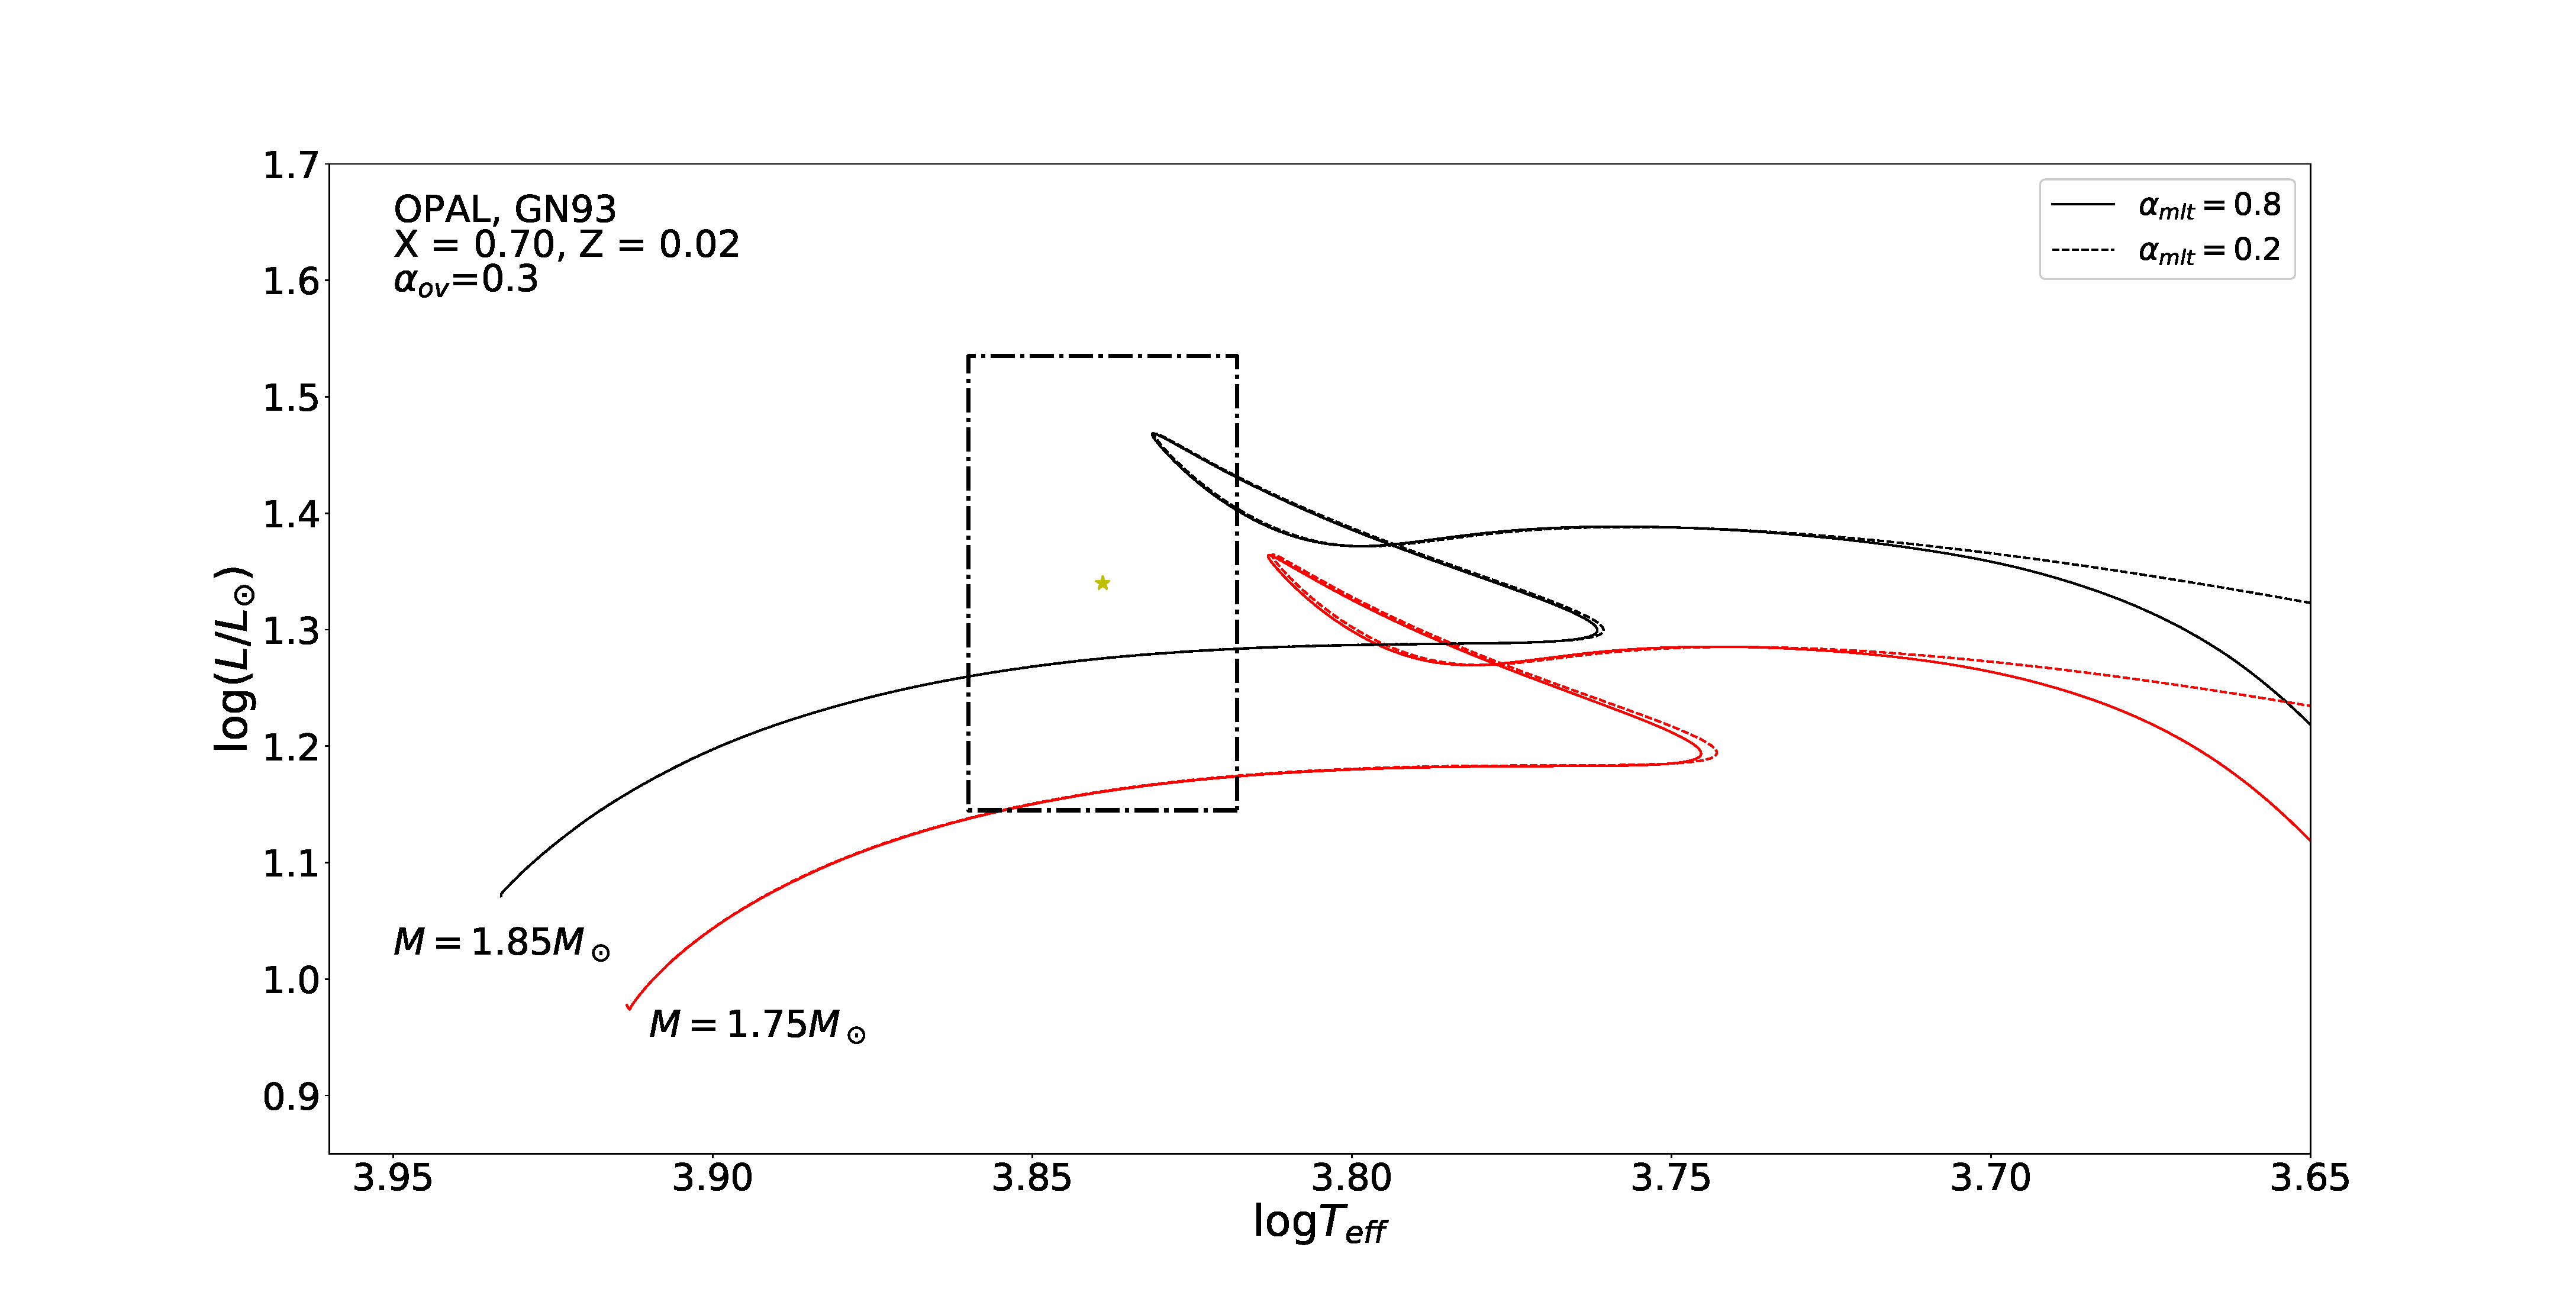
\includegraphics[width=1\textwidth]{mlt.eps}
    \caption{Evolutionary tracks with masses of $M=1.75$\msun and $1.85$\msun and parameter combinations of $X=0.70$,$Z=0.02$, $\alpha_{ov}=0.2$. Each are calcululated with two different mixing lengths of $\alpha_{mlt}=0.5$ (red line) and $\alpha_{mlt}=0.5$ (black line). The black dashed line indicates errobox for uncertainties for observed parameters from \citet{lenz2010delta}.}
    \label{mlt}
\end{figure}

Even though the mixing length paints a nice picture of the convection in the outer layers, there are still issues related to the convection deep in the interior. Specifically to which extend chemical elements are mixed, as it has a big impact on the later evolution of the star. For MS stars with a convective cores the main discussion topic is the convective core overshooting. The convective core overshooting relates to the issue that the boundary between convective core and radiative layers is not sharp; instead, the convection "overshoots" into the layer above (for a quantitative description, see \citet{kippenhahn1990stellar}, Chap. 30). The amount of overshoot depends on the velocity of the convective elements and the breaking force, which are difficult to find as it includes non-local solutions to velocities, gradients and fluxes in the entire core. Therefore, the values for overshooting are, as for the mixing length), arbitrary and can only be evaluated through modeling. 

There are two standard methods that are commonly used to calculate the overshoot numerically. The first one is quite similar to that of the mixing length, describing the extension of the convective region defined by the Schwarzschild criterion, in terms of pressure scale height

\begin{equation}
    l_{ov} = \alpha_{ov}H_p,  
\end{equation}

\noindent in which $\alpha_{ov}$ is typically in the order of 0.1 and 0.2. Even though it resembles the description of the mixing length parameter $\alpha_{mlt}$, it has no relation to it and is purely detemined through comparing models to observations. This prescription is applied as "step overshoot" in MESA. The second method considers convective overshoot as a diffusive process with a diffusion constant depending on the radial distance z from the border defined from the Schwarzschild criterion. 

\begin{equation}
    D(z) = D_0 \exp{\frac{-2z}{f_{ov}H_p}},
\end{equation}

\noindent where $f_{ov}$ is a free parameter in the order of 0.02, and $D_0$ sets the scale of the diffusive speed. This prescription has a particular advantage as it can be added quite easily to a stellar evolution code where diffusion is already implemented. However, for this work, only the former prescription is implemented.

The reason that convective core overshoot is important to implement is that the overshoot causes additional mixing of elements. Hence, more hydrogen is transported to the core, acting as additional fuel on the main sequence. Therefore, just a small extension to the convective core causes a significant continuastion of the main sequence. An example can be seen on \figref{ov_example}, where two stellar evolution tracks of masses 1.95\msun and 1.75\msun are shown. The black line indicates a track with $\alpha_{ov}=0.2$ and the red line the corresponding track with $\alpha_{ov}=0.3$. it can here clearly be seen that the main sequence is significantly longer for models with higher $\alpha_{ov}$, and that it affects the remaining part of the evolution as well. 

\begin{figure}[htbp]
    \centering
    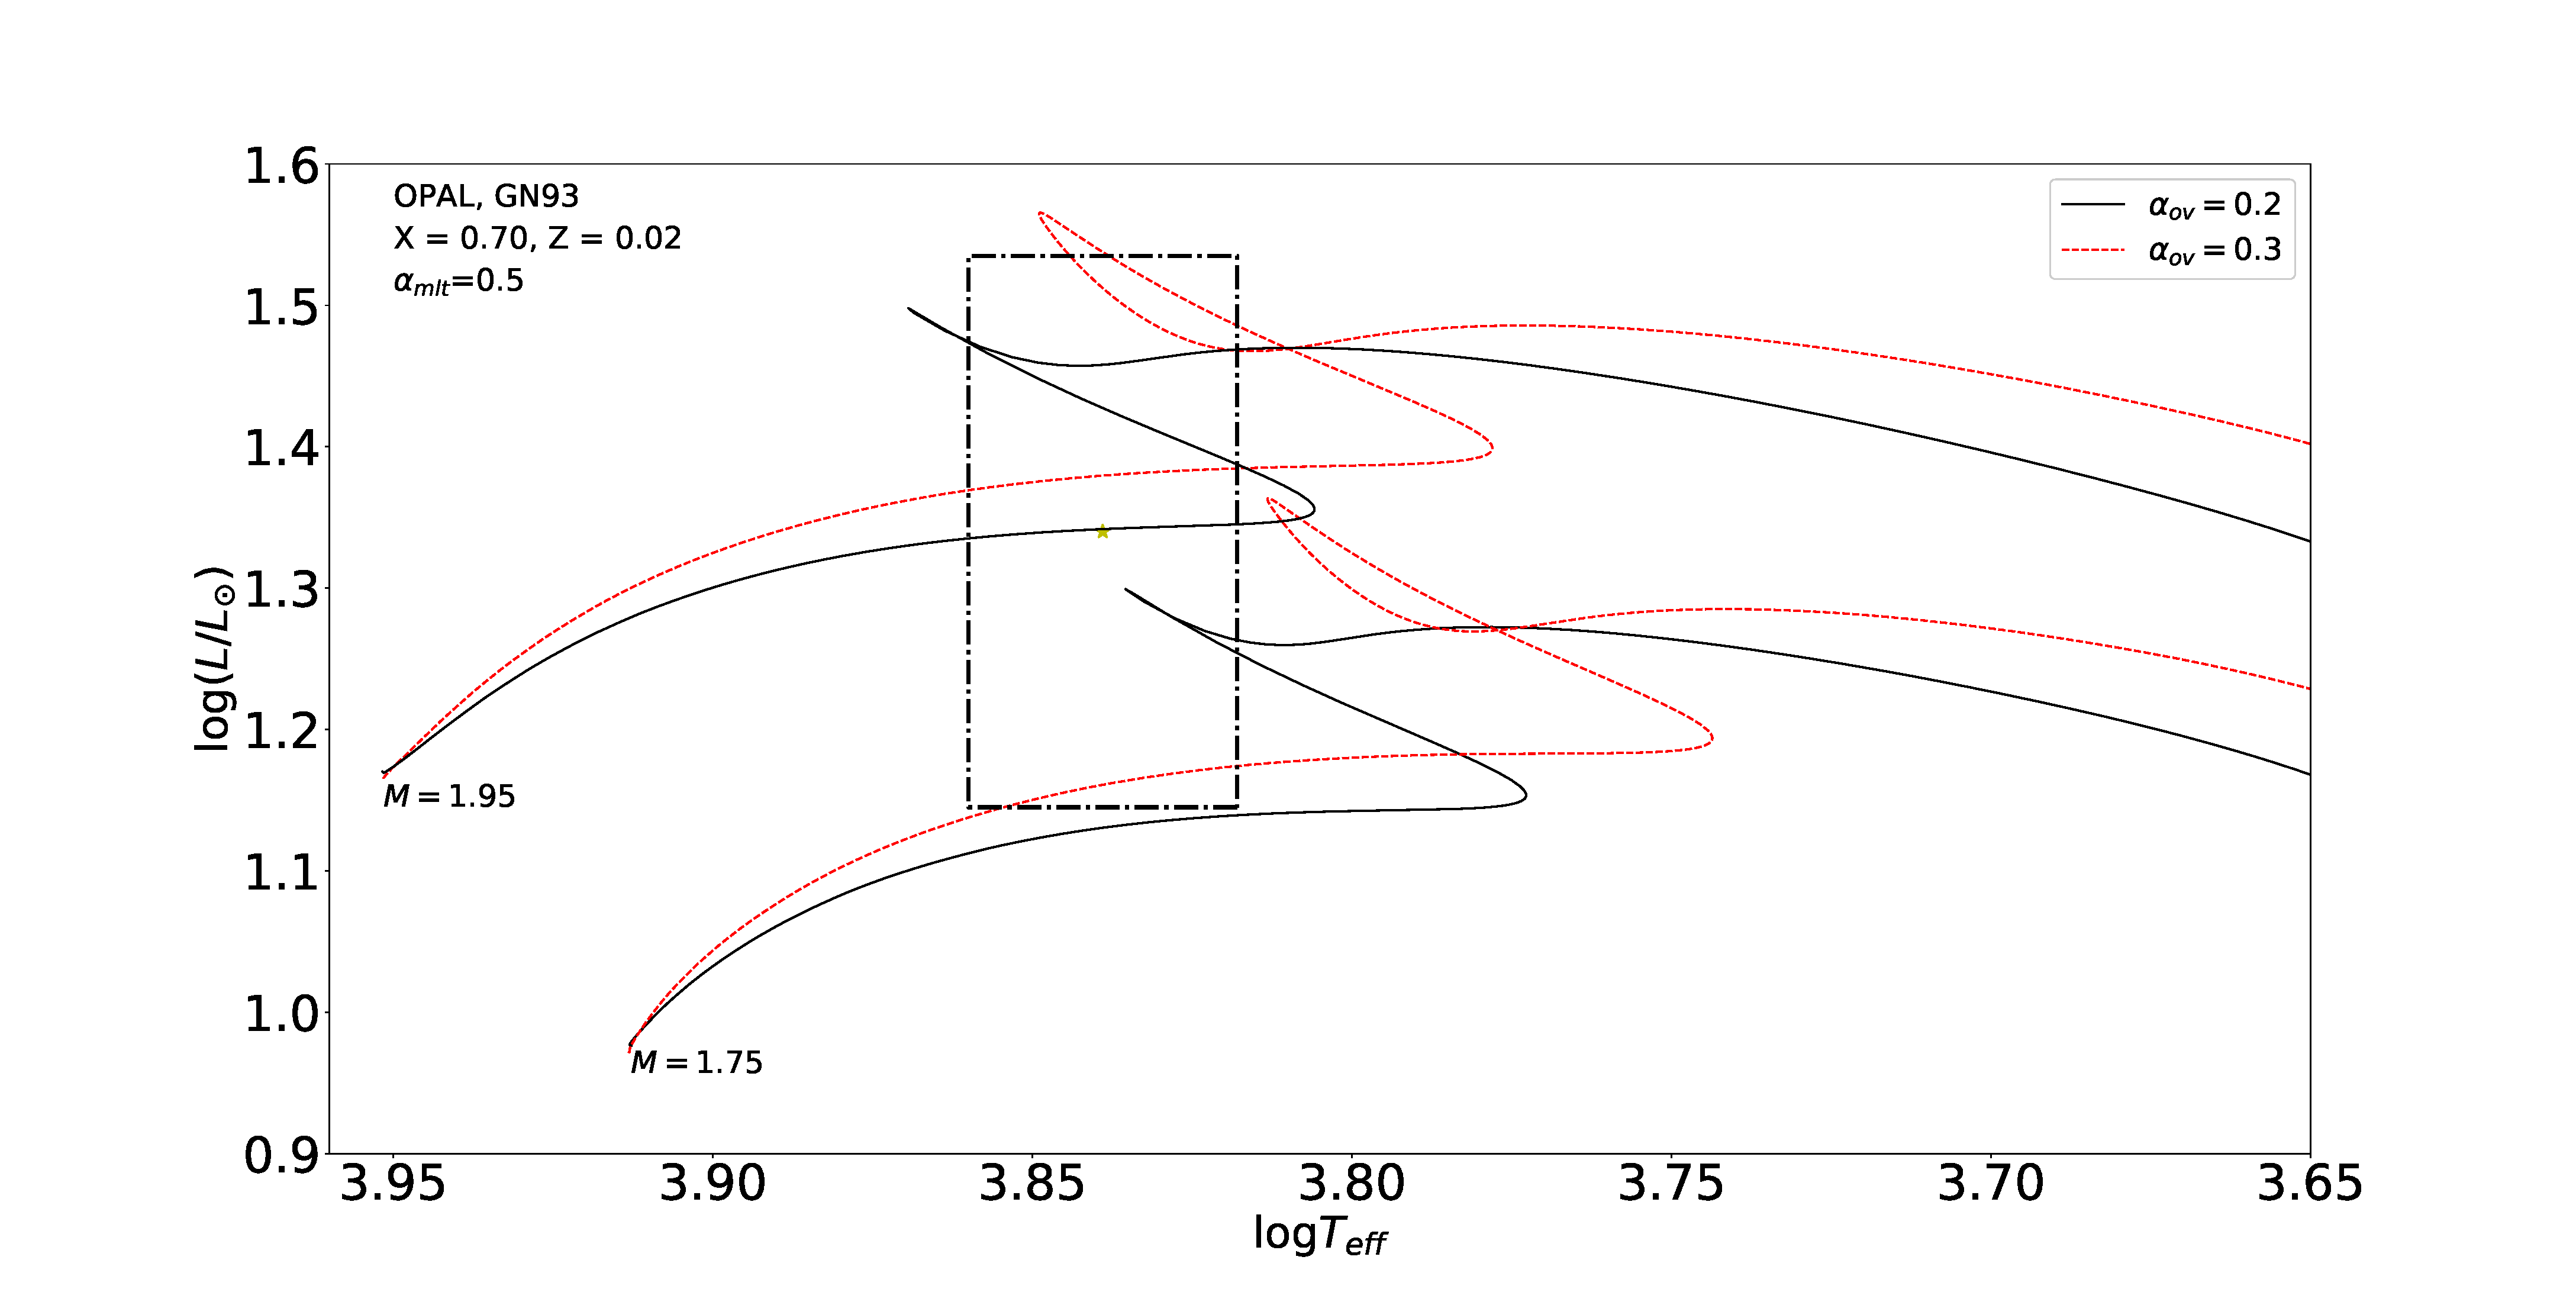
\includegraphics[width=1\textwidth]{overshoots_example.eps}
    \caption{Evolutionary tracks with masses of $M=1.75$\msun and $1.85$\msun and parameter combinations of $X=0.70$,$Z=0.02$, $\alpha_{mlt}=0.5$. Each are calcululated with two different mixing lengths of $\alpha_{ov}=0.3$ (red line) and $\alpha_{ov}=0.2$ (black line). The black dashed line indicates errobox for uncertainties for observed parameters from \citet{lenz2010delta}}
    \label{ov_example}
\end{figure}
\subsection{Element abundance mixtures}

In order for \texttt{MESA} to calculate a stellar model, the element abundances needs to be implemented. The chemical composition of a star is assumed to be a reflection of the distribution of elements in the cloud from which the star was born, assuming that the composition is preserved in the outer layer of the star. %Photospheric observations have revealed that abundance patterns of regular $\delta$ Sct stars are similar to those of the solar neighbourhood \citep{}
Since solar neighbourhood abundances are usually more accurately measured than stars outside, the solar element mixture is commonly used for modeling stars from outside the neighbourhood as well. In MESA, the initial abundances X (hydrogen), Y (helium) and Z (metals, i.e. all elements with atomic numbers higher than helium) is given in terms of mass fractions where $1=X+Y+Z$ must always be fulfilled. 

The solar element abundances depends on the choice of theoretical atmosphere model. Hence, they are updated continuously as atmosphere models are changed and improved. There are several abbreviations of element mixtures that can be appliued in \texttt{MESA}, such as GN93 \citep{grevesse1993cosmic}, GS98 \citep{grevesse1998standard} and a09 \citep{asplund2009chemical}. %The most commonly used solar element abundances are GN93. The solar mass fractions for thise abbreviations are given in \tabref{tab:solar}
\citet{grevesse1993cosmic} used a one-dimensional hydrostatic atmosphere model to derive the solar abundances, and compared to the solar system abundances extracted from meteorites, and found good agreement. This is what is used in this project. The main reason for this is that compared to a09, GN93 does not have issues such as \textit{the solar abundance problem}\citep{asplund2009chemical}. The importance of element mixture choice is further discussed in \secref{sec:discussion}. 

\subsection{Equation of state}

The equation of state takes the density and temperature and calculate the corresponding pressure, ionization degrees and thermodynamic quantities necessary to calculate the stellar structure. 

The equation of state is implemented through the \texttt{EOS} module, where density $\rho$ and temperature $T$ are treated as independent variables in the Helmholtz free energy formulation. However, some calculations are carried out through the Gibbs free energy formulation where the density can be provided through root-finding. This is computationally heavy, so the roots are therefore pre-processed, creating $P_{gas}$ and $T$ tables that allows for a quicker solution when calling the \texttt{EOS} module (provided that the input values are within the range of the pre-computed values). The $\rho-T$ tables are based on OPAL EOS tables from \citet{rogers2002updated}, and for lower values \citet{saumon1995equation}, covering an area up to $Z \leqslant 0.04$. If parameters are outside of the region covered by the \texttt{MESA} tables, the EOS from HELM \citep{timmes2000accuracy} and PC \citep{potekhin2010thermodynamic} are used. These use a free energy approach assuming complete ionization, which is applicable to the region outside of the tables (where cooler stars are only partly ionized). 

\subsection{Opacity data}

From the density, temperature and chemical composition, the EOS yields estimates on the ionization equilibrium concentrations and level populations in a medium. These can be used to evaluate the Rosseland mean opacities. These are implemented though the \texttt{kap} module in \texttt{MESA}, where pre-processed opacity tables are within the \texttt{make\_kap} module. The electron conduction opacity
tables are based on \citet{cassisi2007updated}. For the radiative opcaities, low temperature regions ($\log T \leqslant 4$) is covered by \citet{freedman2008line} or \citet{ferguson2005low}.

Radiative opacities have been calculated by two teams, OPAL and OP. The references for the groups are listed in \tabref{opaci}

\begin{table}
	\centering
	\caption{References for the two opacity groups.}
	\label{opaci}
	\begin{tabular}{ll}
		\toprule
		Source               & Reference \\
		\midrule
		OPAL                 &   \citet{iglesias1996updated}        \\
		OP (Opacity Project) &  \citet{badnell2005updated}       \\ 
		\bottomrule
	\end{tabular}
\end{table} 

Both groups uses slightly different methods to compute the radiative opacities \citep{seaton2004comparison}. For this project, only the OPAL opacities are implemented, which will be discussed briefly in \chapref{sec:discussion}. 
\section{GYRE}
\label{sec:gyre}

In order to interpret asteroseismic observations from recent mission such as MOST \citep{walker2003most,matthews2007one}, CoRot \citep{michel2008first} and Kepler \citep{borucki2009transiting, gilliland2010kepler}, a stellar oscillation code calculating
the eigenfrequency spectrum of an input stellar model is needed. 
The asteroseismic module included in \texttt{MESA} is based on the stellar pulsation code \texttt{ADIPLS} \citep{christensen2008adipls}, which allows for a calculation of the eigenfrecuencies. However, a demand for more detailed non-adiabatic calculations lead to the development of \texttt{GYRE}, which is an open source pulsation code from 2013 described in  \citep{townsend2013, townsend2017} and on the webpage \citep{bitgyre}. 

\texttt{GYRE} is written in \texttt{Fortran 2008} and uses a \textit{Magnus Multiple Shooting} (MMS) scheme to solve linearized pulsation equations. The following steps are used to calculate the eigenfrequencies for an arbitrary input model:

\begin{enumerate}
    \item \emph{Stellar model} As a first step, \texttt{GYRE} needs to read an input model. This model can be either read from a pre-built or can be constructed analytically. It supports three different classes of models. The first is the evolutionary models (which is what is used in this work) constructed from a stellar evolution code. The second relies on polytropic models, and the last is purely analytical calculations based on explicit expressions for structure coefficients. 
    \item \emph{Grid calculation} When the file has been read, a calculation grid is constructed. The grid allows for multiple shooting and eigenfunction reconstruction. The type of grid idepends on the type of input model. 
    \item \emph{Root-finding} Initial guesses for discriminant roots are found by scanning the frequency space in the grid. 
    \item \emph{Eigenfunctions} Based on the initial guesses of roots, the corresponding eigenfunctions are then constructed. 
\end{enumerate}

These are only the very basic steps used by \texttt{GYRE}; a more detailed description of the numerical steps used is beyond the scope of this work, and the reader is instead referred to \citep{townsend2013}.

It is now also possible for \texttt{GYRE} to be implemented directly in the \texttt{MESA star} module, which couples calculations of both stellar evolution and frequencies. However, implementing it is a bit more intricate than reading in the files separately; therefore, the first method is used in this project (calculating a grid of models that can then be used as an input for the \texttt{GYRE} calculations). 

\subsection{Input and output options}

\texttt{GYRE} reads input parameters given in an input file. The input file is structured in a similar way as the \texttt{MESA} inlist files, consisting of several namelist groups: 

\begin{itemize}
    \item \emph{Constants} Defines the physical constants such as the gravitational constant and solar parameters (mass, luminosity etc.)
    \item \emph{Stellar model} Defines the stellar model that \texttt{GYRE} reads and constructs eigenfrequencies for. 
    \item \emph{Mode parameters} Defines mode parameters such as $l,m$ and minimum and maximum radial orders. 
    \item \emph{Oscillation parameters} Defines the parameters relates to the oscillation, such as inner and outer voundary conditions and rotation. 
    \item \emph{Numerical parameters} Specifies numerical methods parameters. 
    \item \emph{Frequency scan} Defines the span of the frequency space scan with a set of points. 
    \item \emph{Calculation grid} Defines the parameters used for the calculation grid. 
    \item \emph{Output files} Specifies the output produced by the end of a run. This includes the file format, frequency units, comma separation etc.  
\end{itemize}

For this project, the input model is constructed as a .GYRE file for every profile constructed in \texttt{MESA}, which is then read into the \texttt{GYRE} input file. The input files used in this project for 44 Tau and Superstar is constructed from a bash script which can be seen in \secref{inlist}. When the input file has successfully been read and the calculations have finished, \texttt{GYRE} constructs one of two different types of ouput files. The first is the Summary files that provides global information on the theoretically produced modes. The second is the mode files, containing information on a single mode including detailed eigenfunction quantities such as rotation kernels. For this project, the first file is used. The contents of the output file is defined in the input file described above with the \texttt{summary\_item\_list} (or, correspondingly \texttt{mode\_item\_list}). The most relevant for this project is the harmonic degree, radial order and frequencies. Options for non-adiabaticity can be included in the \texttt{GYRE} calculations and will be discussed in \chapref{sec:discussion}.

%Several options for non-adiabaticity can be included in the \texttt{GYRE} calculations. This has the advantage that it yields the excited frequency range which can be compared to observations. One of the major contradictions between observations and theory in asteroseismology is that theory predicts all frequencies to be excited if the pulsations are driven by the kappa mechanism. But unfortunately, this is not what is observed, Therefore, using non-adiabatic calculations can provide a more detailed information on the excitation of each mode. However, the major disadvantage of this is that since non-adiabatic equations rely on solving non-linear equations, the calculation time increases significantly from that of adiabatic calculations. Especially if it needs to be done for an entire grid. Therefore, this option is not used in this work.  
\chapter{Modeling 44 Tau and Superstar}
\label{modeling}
In this chapter the process of modeling the stars 44 Tau and Superstar in MESA and GYRE is described. The methods for comparing the models to  observations is introduced and discussed.

\section{Choosing a grid}
\label{sec:grid}
For this project models are created in order to compare to observations and ultimately narrow down the parameter space for 44 Tau and HD 187547. More than one approach can be taken in order to reach this goal, each with their own advantages and disadvantages. \citep{lenz2010delta} narrows down the grid size by first calculating the best mass for each stage. I.e. it is an approach where the star is assumed to be in either ms, post-ms contraction or post-ms expansion phase, and these results in three different grids where the best model is found for each stage. This method has the advantage that is it forces a result on all the relevant possibilities. However, it is a process that requires the grid to be narrowed through several steps, including a separate analysis of the mass range. 

In this project, a slightly different approach is used. Instead of dividing the models into different stages and narrowing it down, a wide grid stretching over the entire instability domain is calculated, and of these the best models are found. To find not only the best overall model, but also consider their tracks and initial input parameter combination, the best model for each track is found. This choice is discussed in \secref{bestmodel}. 

As discussed in \secref{compute}, the initial set of parameters chosen has a great influence of the further evolution of the star. Therefore, a grid needs to be chosen with care in order to get a big enough grid to not only cover the observationally determined parameter space, but adequately beyond this in order to include the uncertainties on the observations.
Since the mass has not been observationally determined, a good place to start is the instability strip. Usually, the intermediate mass stars have masses between 1.5-2.5 \msun in order to cover the strip where pulsations are expected. Therefore this mass range is chosen to be from 1.5\msun to 2.2 \msun, where the most important part is to include masses all the way down to 1.5\msun since these star in particular mark the transition to convective cores. The  initial abundances are chosen to be within the numerical boundaries of \texttt{MESA}, as discussed in \chapref{compute}. This yields a range of 0.65<X<0.70 and 0.01<Z<0.03. Numerical results for two different masses and $Z$ can be seen on \figref{diffz}. Here, the red color correspond to masses of $M=1.75M_\odot$ and black lines $M=1.85M_\odot$. The different values of $Z$ are represented with full and dashed lines respectively. There is a clear difference between tracks with different $Z$. Higher values of $Z$ yields a high opacity which blocks the radiation from the inner layers. Hence, stars with higher metallicity will be less luminous. In this case, the luminosity difference is in the order of \l = 0.2 within the three sigma uncertainties on the luminosity.  

\begin{figure}[htbp]
	\centering
	\includegraphics[width=0.9\textwidth]{test_z_2.png}
	\caption{Stellar evolution tracks for two different masses with two different metal abundances. Each track has $X=0.70$, $\alpha_{mlt}=0.5$ and $\alpha_{ov}=0.3$. The red lines indicates tracks with masses of $M=1.75M_\odot$, and black lines indicate $M=1.85M_\odot$. The full lines have $Z = 0.03$ and dashed lines $Z = 0.01$. The black dashed box shows the three sigma uncertainties on \l and \teff (from \citet{lenz2010delta}). }
	\label{diffz}
\end{figure}

Numerical results for the initial hydrogen abundances can be seen on \figref{diffx}. The line and color convention corresponds to that of \figref{diffz}, with the difference being the line type indicating the values of $X$ instead. Here it is also clear that the initial hydrogen abundance affects the luminosity (however less than the $Z$). Higher hydrogen abundances causes a smaller helium abundance (when $Z$ is held constant) HVORFOR ER LUM STØRRE?. 

\begin{figure}[htbp]
	\centering
	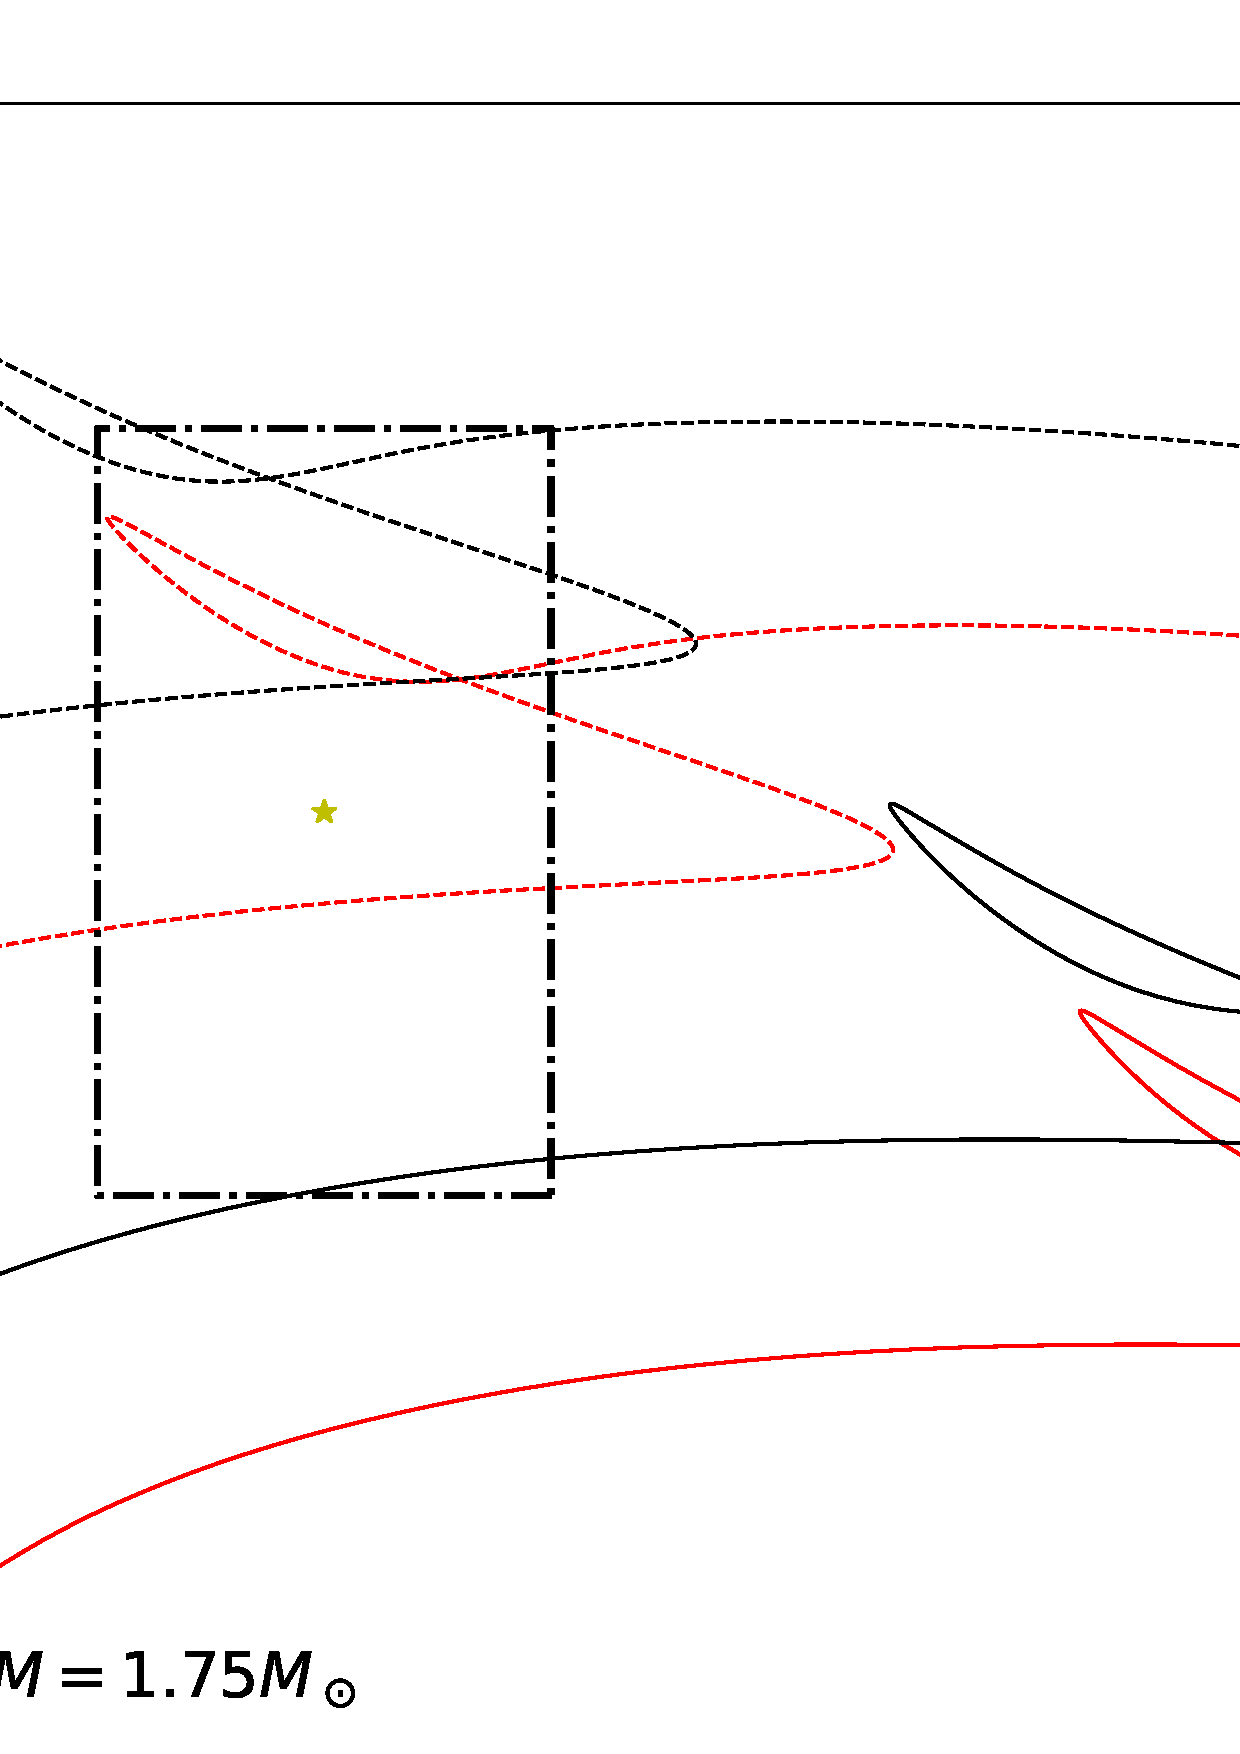
\includegraphics[width=0.9\textwidth]{test_x.png}
	\caption{Stellar evolution tracks for two different masses with two different metal abundances. Each track has $Z=0.01$, $\alpha_{mlt}=0.5$ and $\alpha_{ov}=0.3$. The red lines indicates tracks with masses of $M=1.75M_\odot$, and black lines indicate $M=1.85M_\odot$. The full lines have $X = 0.65$ and dashed lines $X = 0.75$. The black dashed box indicates the three sigma uncertainties on \l and \teff (from \citet{lenz2010delta}).}
	\label{diffx}
\end{figure}

 $\alpha_{mlt}$ and $\alpha_{ov}$ are parameters that are not easily chosen, since they are purely empirical and depend strongly on the prescription used in the modeling (see \secref{sec:conv_prescriptions}. For the $\alpha_{mlt}$ the standard value in \texttt{MESA} is around 1.8. The Warsaw-New Jersey stellar evolution code used to calculate models for 44 Tau by \citep{lenz2010delta} has the same mixing-length prescription as \texttt{MESA}. Their results showed that models with mixing length of $\alpha_{mlt} > 0.2$ gave the best fits, confirming the assumption that smaller mixing lengths than the sun is needed in order to model these stars. However, \texttt{MESA} is not computationally capable of handling a mixing length below 0.2 which is not surprising as it would mean that energy transport by convection in the outer layers is almost non existing. This also underlines the fact that convection is treated differently in each stellar evolution code, and parameters such as $\alpha_{mlt}$ needs to be carefully examined in the grid. It can also be argued that since $\delta$ Sct stars have a much smaller convection layer than that of the Sun, the convection will not be as efficient.  \citet{trampedach2011mass} calculated a range of mixing lengths through a grid simulation of solar type structures. One of the results can be seen on \figref{tramp}. 

\begin{figure}[htbp]
	\centering
	\includegraphics[width=0.8\textwidth]{tramper.png}
	\caption{Mass mixing lengths in units of pressure scale height $H_p$ in the \teff - $\log g$ plane. \citep{trampedach2011mass}.}
	\label{tramp}
\end{figure}

The mixing length is predicted to be smaller for higher values of \teff, as expected. Both 44 Tau and HD 187547 are out of range in \teff space, since the mixing length range here is calculated based on solar-like structures. However, the trend in mixing length is still applicable to intermediate mass stars. As an initial grid we therefore choose values of $\alpha_{mlt}$ between 0.2 and 0.8. Analogous to the mixing length, the convective overshoot near the core is described with the convective core overshoot parameter $\alpha_{ov}$. As it is typically in the order of 0.1-0.2 \citep{kippenhahn1990stellar}, we here choose values between 0.1-0.3.  

Some models in the grid were not possible to compute with the current equations in MESA. For 1.5\msun it was not possible to compute models with a metallicity higher than 0.02, it the initial He abundance is low. For 1.80\msun three tracks were excluded as they could not be computed either. The initial grid used here can be seen in \tabref{grid}.
\begin{table}[htbp]
  \centering
  \caption{Values and step sizes for all parameters in the grid calculated in this work. }
  \label{grid}
  \begin{tabular}{|l|ll|}\toprule
    & values    & stepsize \\ \midrule
    X                         & 0.65-0.75 & 0.05     \\
    Z                         & 0.01-0.03 & 0.01     \\
    Mass/\msun                & 1.5-2.2   & 0.05     \\
    $\alpha_{mlt}$            & 0.2-0.8   & 0.3      \\
    $\alpha_{ov}$             & 0.1-0.3   & 0.1      \\ \bottomrule
    \end{tabular}
\end{table}

Some of these combinations did however not converge properly, and could therefore not be included in the grid. These models are:
\begin{itemize}
	\item $M=1.50M_\odot$: combinations with $X=0.75$ and $Z=0.02$ or $Z=0.03$
	\item $M=1.55M_\odot$: combinations with $X=0.75$ and $Z=0.03$
	\item $M=1.95M_\odot$: combinations with $X=0.75$ and $Z=0.03$
	\item $M=1.80M_\odot$: combinations with $X=0.75$ and $Z=0.02$ and $\alpha_{mlt} = 0.2$
	\item $M=1.90M_\odot$: combinations with $X=0.75$ and $Z=0.02$ and $\alpha_{mlt} = 0.8$ 
\end{itemize}

It is unclear why these exact combinations have numerical issues, since it would require an investigation beyond the scope of this work. However, they all have in common that the initial hydrogen abundance is very high at $X=0.75$. This might explain most of the issues since this value is in fact higher than the initial value of the interstellar medium it was born in, which can practically never be true. However, the reason for still including them is that models might still reproduce these high values due to the numerical calculations. So if a model has this value it can be interpreted as an example of the imperfect theory behind the codes.  

\section{Resolution and varcontrol}
\label{sec:res}

As mentioned previously in \secref{sec:mesa}, they way MESA works is to fulfill calculations in time steps that are non-equidistant. As a result of this, models on a track can be far apart if the evolution is fast. This means that models on the main-sequence are well resolved, while the models on fast stages (particularly post-ms contraction phase) are fare apart in terms of structure. Since every model calculated in MESA yields one model in GYRE, this also results in the frequencies being very different from one model to another, which should be considered when calculating the \chis (see \secref{sec:chis}). An example can be seen on \figref{resstage} where, the radial fundamental mode is plotted as a function of timestep. The lower panel of \figref{resstage} is the same models corresponding to middle panel but where the radial fundamental mode frequency difference between models, $f_1(i+1) - f_1(i)$, is plotted as a function of time. This shows that the resolution in the frequency space is as high as ~0.18 cyc/day for this track (some tracks go up to ~0.2). The highest point is, however, in the very beginning of the main sequence, and not on the post-main sequence contraction phase, where it is favorable to have a high resolution.     

\begin{figure}[htbp]
    \centering
    \includegraphics[width=1\textwidth]{resolution_stages.png}
    \caption{Resolution at different stages of an evolution of a track with M=1.85\msun, X=0.75, Z=0.02, $\alpha_{mlt} = 0.5$, $\alpha_{ov} = 0.3$. The begininng of the main sequence is marked with a bold "1", continuing until "2" where the post-main sequence contraction phase starts. At "3" all hydrogen has been exhausted in the core, and the star is in the post-main sequence expansion phase. Middle panel: Here the fundamental frequency is plotted as a function of time. The dashed lines indicate the stages corresponding to those in the middle panel. Lower panel: Shows the absolute difference in fundamental frequency between two subsequent models.}
    \label{resstage}
\end{figure}

Since 44 Tau has earlier been identified to be in the post-ms contraction phase (and since we cannot exclude that possibility for Superstar either) the resolution of the models in MESA needs to be adjusted to allow for a higher chance of finding a good fit. It is possible to simply force smaller timesteps, but this is not ideal since it would not only increase the computation time on the fast evolutionary stages, but the entire track. Since a better resolution is not really needed on the ms, it is therefore better consider an alternative parameter that does not waste computation in areas where it is not needed. 

There are more than one way of doing so. It is possible to set a limit for magnitude of max change in temperature and photosphere with the \texttt{delta\_lgTeff\_limit}, or alter the minimum and maximum number of grid points in a model with \texttt{mesh\_delta\_coeff} (a higher values decreases number). These parameters need to increase the resolution in the right area, but also within a resonable amount of computation time. The parameter found to be most efficient in this project is the \texttt{varcontrol\_target} parameter. This parameter is assigned a value describing the relative variation in the structure from one model to the next. The timestep then adjust accordingly, depending if the variation is smaller or larger than the value. Increasing the resolution through this value does also increase the computation time, however, reasonably. An example of this can be seen on \figref{varcontrol} where the same track is plotted with different values of \texttt{varcontrol\_target}. It is here found that a value of 5e-5 is sufficient in making the resolution satisfactory for this work. 

\begin{figure}[htbp]
    \centering
    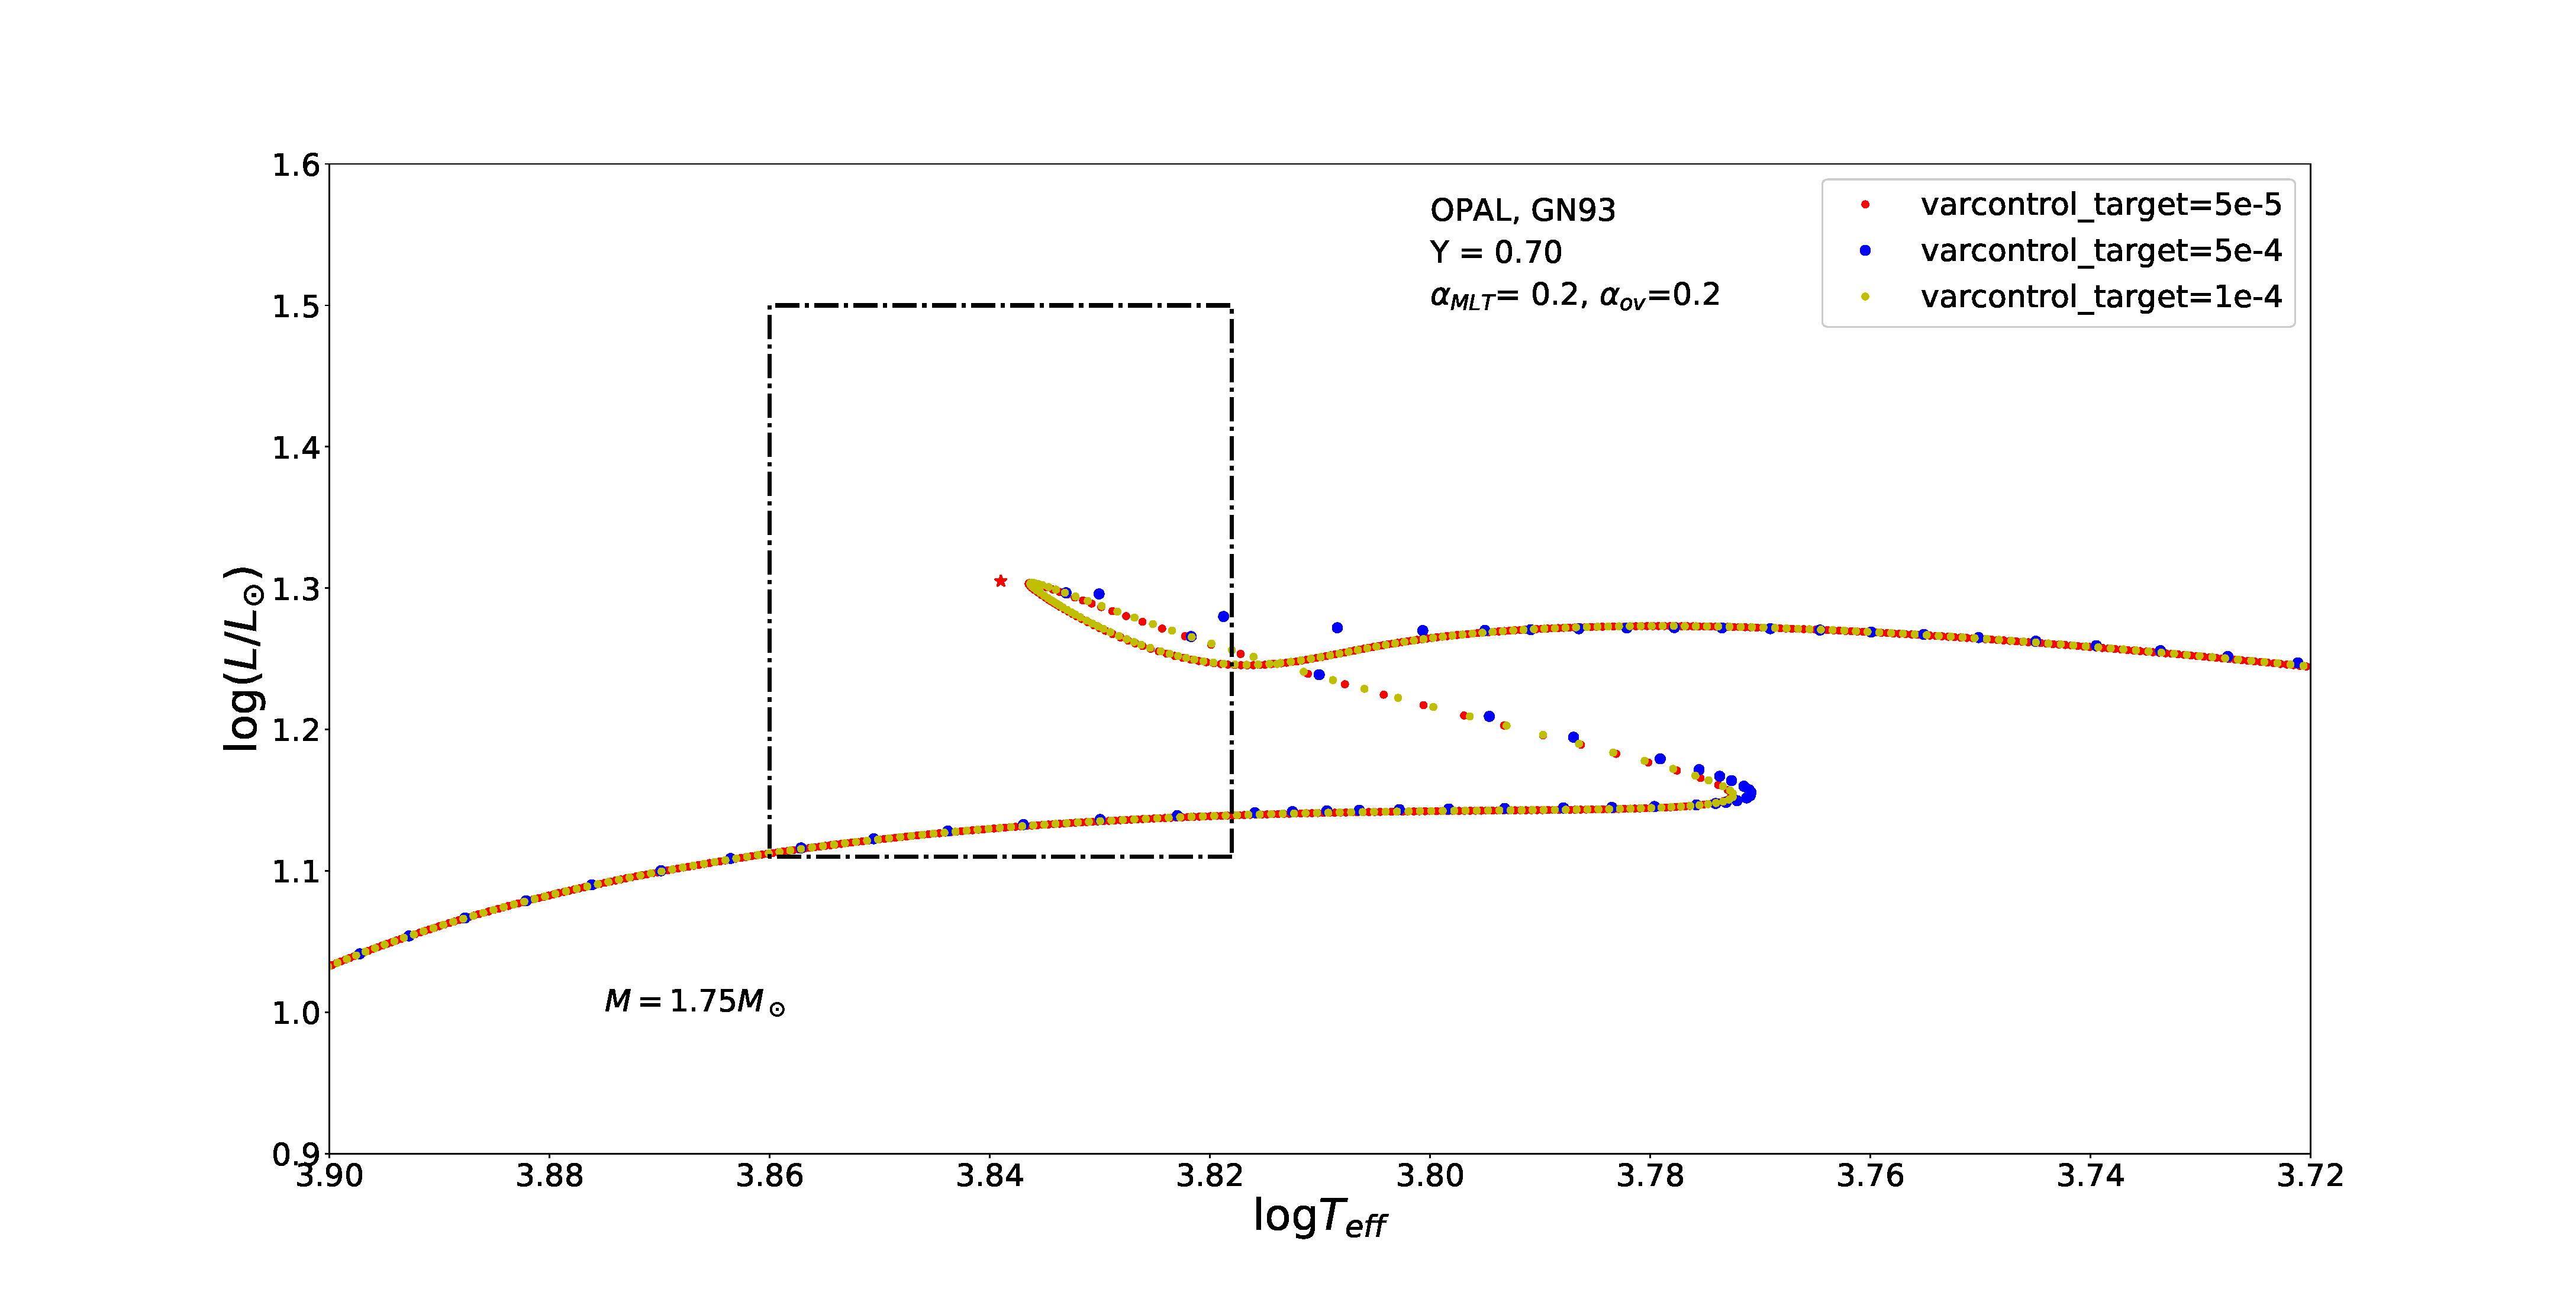
\includegraphics[width=1\textwidth]{varcontrol_res.eps}
    \caption{Evolution of three tracks with same initial parameters, but different values of \texttt{varcontrol\_target} where 1d-4 is default in \texttt{MESA}. It can be seen that the resolution drops significantly for the value 5d-4. Therefore, a slightly smaller value of 5d-5 is chosen for this work.}
    \label{varcontrol}
\end{figure}


Some tracks are still better resolved than others. A general tendency from the computed tracks are that models with overshoot below 0.2 are not resolved nearly as well as models with high overshoot of 0.3, which can also be seen on \figref{ovresol}. Particularly the Henyey hook cannot be reproduced very well for overshoot of 0.1. The details as to why this occurs is beyond the scope of this work, however it is very important to take into consideration when evaluating results as tracks with low overshoot will automatically have fewer models and therefore limited chances of fitting well to observations. 

\begin{figure}[htbp]
    \centering
    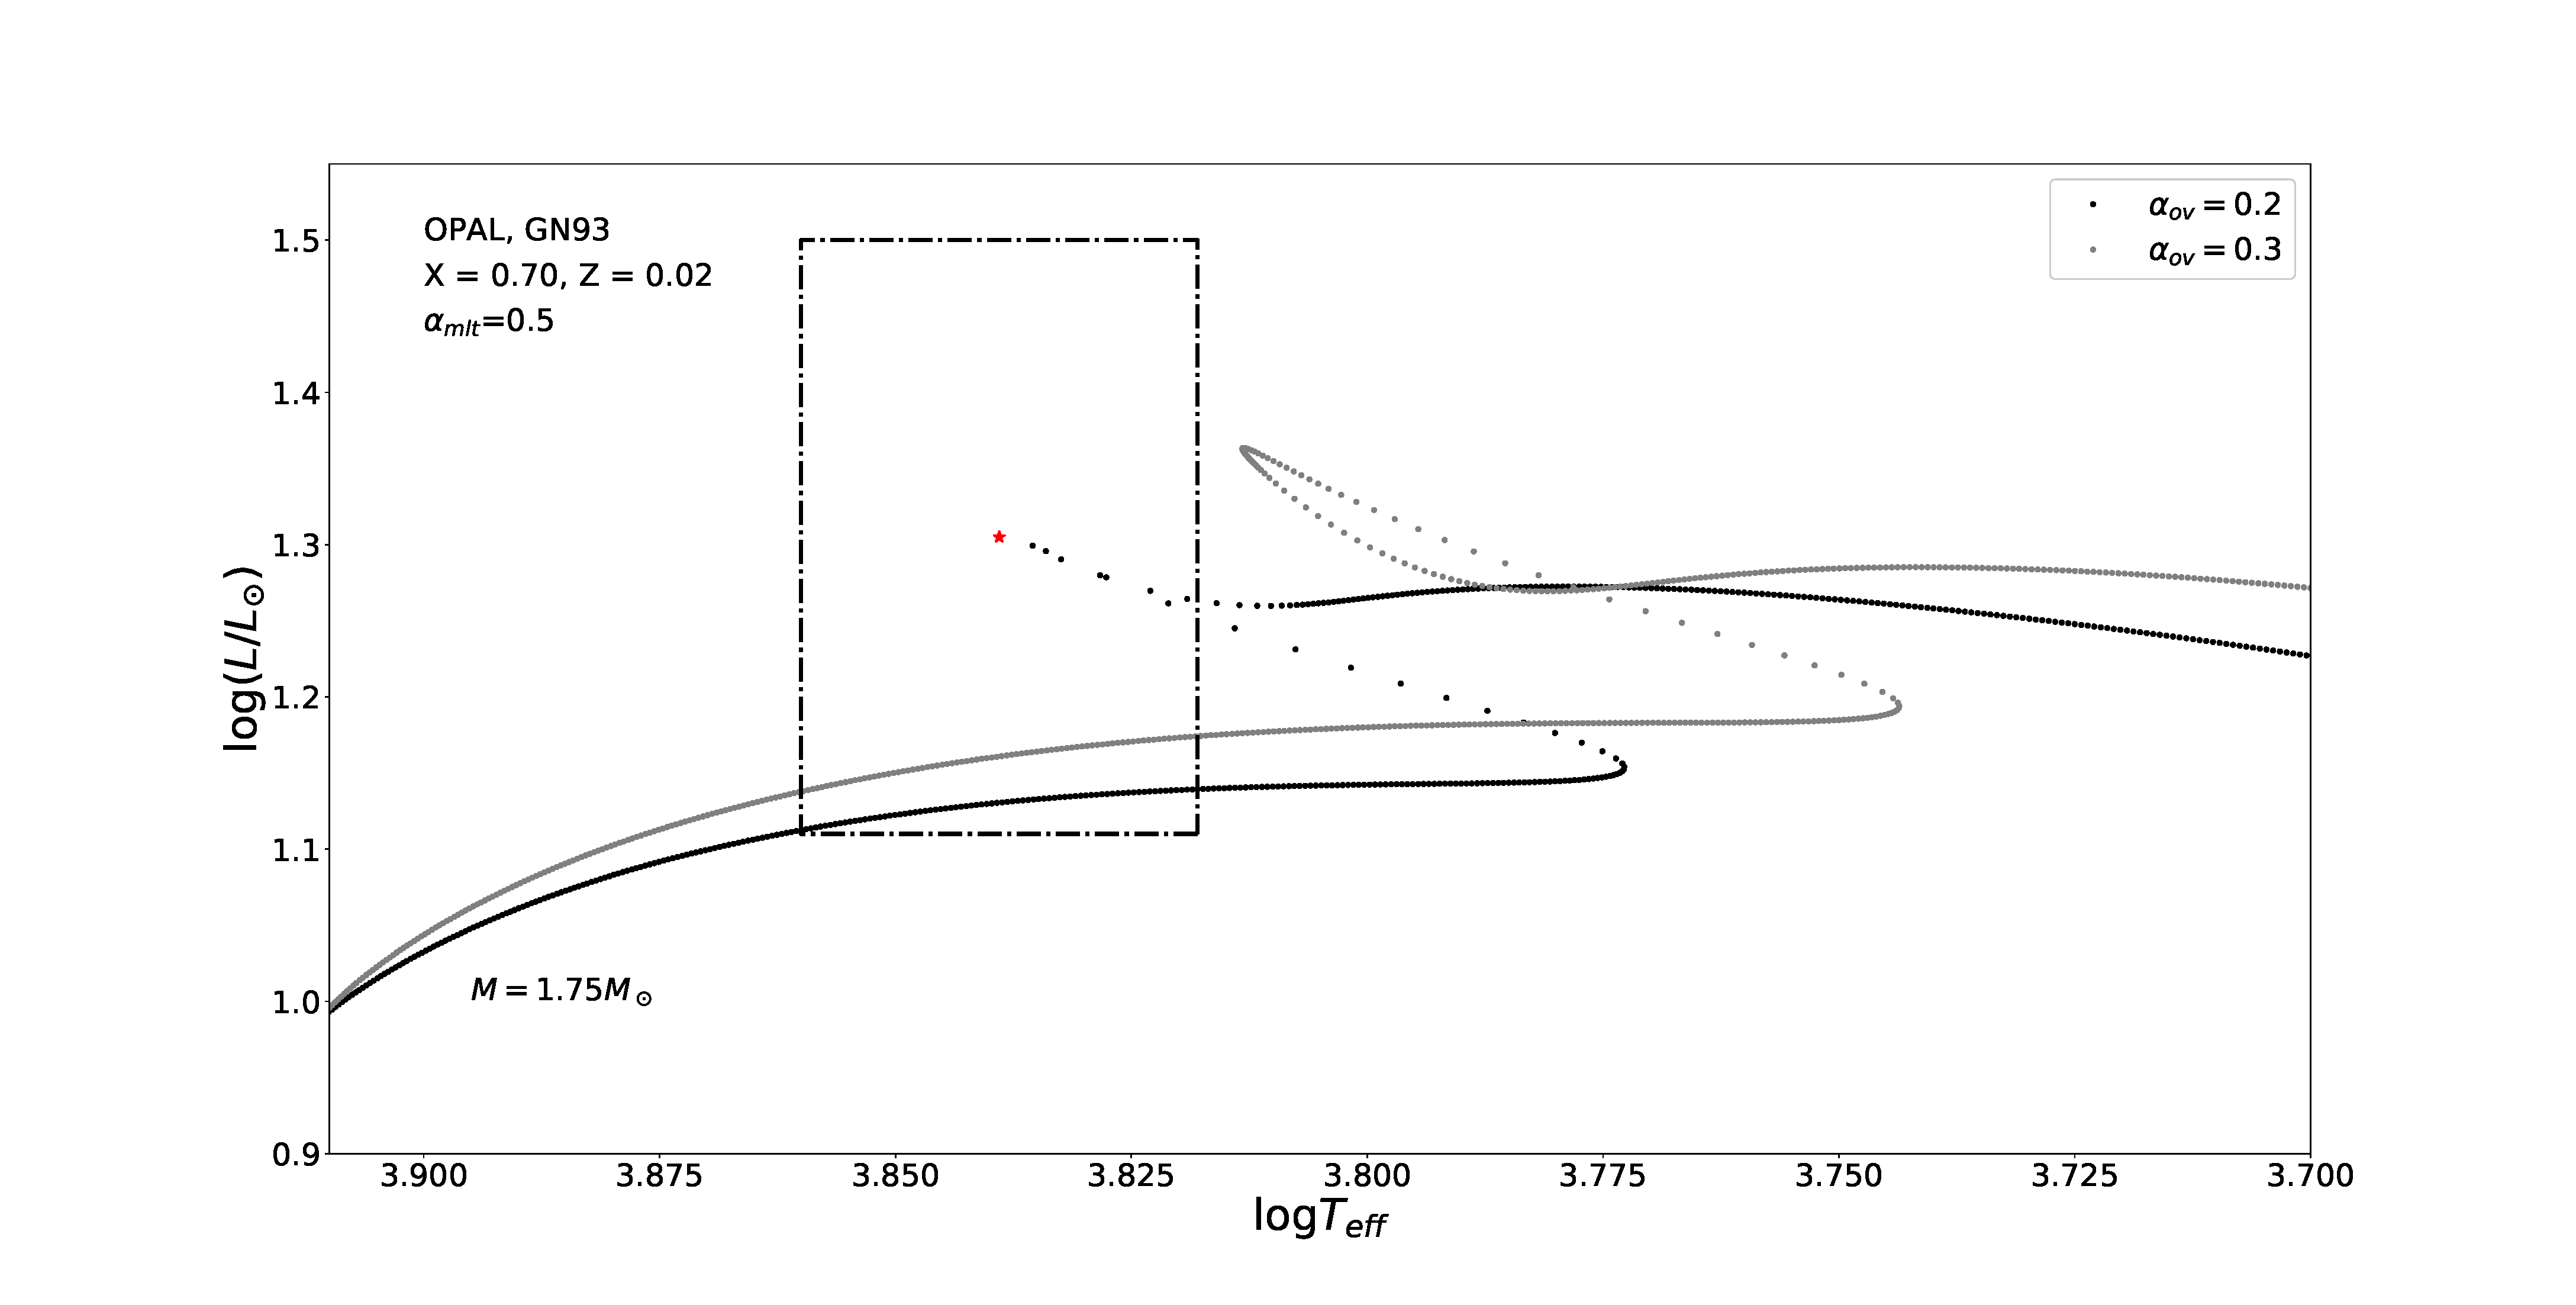
\includegraphics[width=1\textwidth]{resolution_overshoot.eps}
    \caption{Two models of the same track, but with different overshoot.}
    \label{ovresol}
  \end{figure}


\section{chi2 testing}
\label{sec:chis}

\subsection{Finding the best model}
\label{bestmodel}


In order to find out how well/fitted a model is, a comparison with stellar parameters is needed. By just comparing models to luminosity, effective temperature and surface gravity, it is difficult to find an estimate on the evolutionary stage as the best model on one track might be on the main sequence, whereas the best model on a different track is on the post-main sequence. Therefore, frequencies are need as additional observational parameters for comparison (as they, as discussed in \secref{chap:asteroseismology}, change with evolution). There is more than one way of doing the comparisons, but in this work a \chis test is used. \chis yields a value for each models, allowing us to find models with lowest \chis values. The Pearson's goodness of fit test is commonly written as 

\begin{align}
\label{standard_chi}
\chi^2_j = \sum^I_{i=1}\left(\frac{v^{theo}_{i,j}-v^{obs}_i}{\sigma_i}\right)^2,
\end{align}

\noindent where $\nu^i_{obs}$ is the observed parameter for model i, $\nu^i_{theo}$ is the corresponding theoretical parameter and $\sigma^i$ is the uncertainty for the parameter. It provides a number that somewhat describes how close the fitting parameters are tp the corresponding observed parameters. However, there is more than one way of doing a \chis test, as its implementation depends on the work, and particularly the goal that is desired. There are a few assumption that needs to be taken into consideration before implementing a \chis test. Most importantly, statistically speaking, a \chis test does not provide any information on how well individual parameters fit, or how likely a model is to be good. As the goal of this project is to find the most likely evolutionary stage, the \chis values can simply be used as a way of \textit{comparing} between the different models. So models with the lowest \chis are the models with parameters closest to the observed parameters. These thereby provide an age span and a likely evolutionary stage. 
If the \chis values are to be compared between the different models, then they need to be calculated under the same conditions. This means that calculations should be done with the same number of fitting parameters for all models (since they otherwise are not comparable). For instance, if one model have more fitted frequencies than another, the \chis with the model with more fitting parameters will have an extra link, causing it to naturally be larger than the \chis for the model with fewer fitted frequencies, making their \chis incomparable. 

%GYRE produces an output file for the chosen MESA profiles. Since it computationally takes time to produce the output files, a constraint is needed in order to determine which profiles are within the range where we wish to produce a GYRE output file. This is done by defining a parameter space of size three sigma, based on observed parameters \teff, \lum, and \grav.

%In order to test how well the computed frequencies match observed frequencies a \chis prescription is applied to every profile. 
\subsection{44 Tau}
\label{sec:chi44}

\subsubsection{l=0 modes}

For 44 Tau, the frequencies of the fundamental mode and first overtone are well-determined. These frequencies act as a constraint for the l=0 mode models. Initially the l=0 modes are computed using GYRE for the entire grid described in \secref{sec:grid}. Here, we have an initial constraint from only the frequencies corresponding to the radial fundamental mode and first overtone and the global parameters. The \chis for this initial run then becomes

\begin{align}
\chi^2_j & = & \left(\frac{\nu^{\text{fund,obs}}-\nu_j^{\text{fund,theo}}}{\sigma_{\text{fund},j}}\right)^2 
 + \left(\frac{\nu^{\text{first,obs}}-\nu_j^{\text{first,theo}}}{\sigma_{\text{first},j}}\right)^2 
 +
\left(\frac{\text{T}_\text{eff}^{obs}-\text{T}_{\text{eff},j}^{\text{theo}}}{\sigma_{\text{T}_\text{eff},j}}\right)^2 \\
& & +
\left(\frac{\log \text{g}^\text{obs}-\log \text{g}^\text{theo}_j}{\sigma_{\log \text{g},j}}\right)^2 
 + \left(\frac{\log \text{L}^{\text{obs}}-\log \text{L}^\text{theo}_j}{\sigma_{\log \text{L},j}}\right)^2, 
 \label{eq:chis}
\end{align}

\noindent where $\chi^2_j$ is the \chis for the j'th model. For $\text{T}_{\text{eff}}$, $\log \text{g}$ and $\log \text{L}$ the $\sigma$ used is simply the uncertainties from observations. Notice here that even though the frequencies are calculated for the entire track, the \chis is not calculated for models on the pre-main sequence. 

For the frequencies the $\sigma$ is naturally very small (in the order of $10^{-6} \text{Cyc}/\text{day}$, since the uncertainty on observations depend only on the observation time. Long observation times of 44 Tau therefore results in very narrow peaks. It is very nice to know a parameter to this precision, but as shown in \eqref{eq:chis} a small uncertainty will results in high values of \chis. This is not a problem on its own, as the \chis only represent how well the model fits observation. If this value is extremely high it does not necessarily mean that the models are not good models for the star, but that a model precision is simply not comparable to frequency precision. In other words, no model will ever get close to fitting well. Also, by only dividing by the uncertainties the resolution of the track is not taken into consideration. As shown in \secref{sec:res} the resolution of the track is important as fewer models in one area decreases the possibility of having a good fit. This also means that a model frequency can change a lot between two time steps if the resolution is low, and this should be taken into account. In this work the following is prescription is therefore applied to the frequencies: 
\begin{equation}
\label{sigma}
    \chi^2  = \frac{1}{\alpha}\sum^I_{i=1}\frac{\left(v^{\text{obs}}_{i}-v^{\text{theo}}_{i,j}\right)^2}{(\sigma^{\text{obs}}_i)^2 f_i(\Delta\nu_{i,j})}
\end{equation}

\noindent where i in this case is the different frequencies (i.e I=2 for l=0 calculations where we only compare to fundamental frequency and first overtone),j is the j'th model, and $\alpha$ is a scaling parameter. $f_i(\Delta \nu_{i,j})$ is a function that artificially increases the sigmas on the frequencies

\begin{equation}
\label{function}
    f_i(\Delta \nu_{i,j}) = \frac{\nu_j - \nu_{j-1}}{\sigma_{\text{obs},i}},
\end{equation}
 
\noindent where the distance in frequency space is taken into consideration for the j'th model. Smaller distances in the frequency space between model means a higher $f_i(\Delta \nu_{i,j})$, hence, as smaller \chis. Runs both with and without the uncertainty pump will be made to test the difference in the main result. 

%Alternatively, the \chis for the frequencies can be calculated as \eqref{standard_chi}, but with an expanded $\sigma$ similar to that of a standard deviation

%\begin{equation}
%\label{m2}
   % \sigma_{i,j} = \frac{1}{I}\sqrt{\sum_{i=1}^I \left(\nu_{i,j}^{\text{theo}} - \nu_{i}^{\text{obs}}\right)^2}.
%\end{equation}

%There are both advantages and disadvantages for both methods. The first method does take the spacing into consideration, but it follows from this that the since the \chis are artificially enhanced, the scaling between the frequency \chis and rest of the parameters is off by the scaling factor $\alpha$. This can be found by finding the ratio $\frac{\chi_{freqs}}{\chi_{freqs}}$ for each model, j, and finding the mean. This method is slightly more complicated than the second method, however, the second method does not take the spacing in frequency between models into account, and the standard deviation is based only on two different frequencies. The order of magnitude of the \chis is different for the methods, but as mentioned earlier the numbers themselves are not representative of how well a model fits. 

As of yet only l=0 modes have been fitted. Calculating corresponding l=1 and l=2 modes for all models is time consuming, and therefore a selection criteria is needed. This is done by first finding the model with the lowest \chis is for each track. From all of these the best 5\% are found for both methods, respectively. These models and their initial parameters are shown in \tabref{bestchi_m1} and \tabref{bestchi_m2}. 

\begin{table}[htbp]
  \caption{hest}
  \label{bestchi_m1}
  \begin{tabular}{lllllllllll}
 Model & X & Z & Y & $M[M_\odot]$ & $\alpha_{mlt}$ & $\alpha_{ov}$ & $\log \text{T}_\text{eff}$  & $\log \text{L}$  & $\log \text{g}$ & $\chi^2 (method 1)$ \\
 &  &  &  &  &  &  &  &  &  &  \\
 &  &  &  &  &  &  &  &  &  &  \\
 &  &  &  &  &  &  &  &  &  &  \\
 &  &  &  &  &  &  &  &  &  &  \\
 &  &  &  &  &  &  &  &  &  &  \\
 &  &  &  &  &  &  &  &  &  &  \\
 &  &  &  &  &  &  &  &  &  &  \\
 &  &  &  &  &  &  &  &  &  &  \\
 &  &  &  &  &  &  &  &  &  &  \\
 &  &  &  &  &  &  &  &  &  &  \\
 &  &  &  &  &  &  &  &  &  &  \\
 &  &  &  &  &  &  &  &  &  &  \\
 &  &  &  &  &  &  &  &  &  &  \\
 &  &  &  &  &  &  &  &  &  &  \\
 &  &  &  &  &  &  &  &  &  &  \\
 &  &  &  &  &  &  &  &  &  &  \\
 &  &  &  &  &  &  &  &  &  &  \\
 &  &  &  &  &  &  &  &  &  &  \\
 &  &  &  &  &  &  &  &  &  &  \\
 &  &  &  &  &  &  &  &  &  &  \\
 &  &  &  &  &  &  &  &  &  &  \\
 &  &  &  &  &  &  &  &  &  &  \\
 &  &  &  &  &  &  &  &  &  &  \\
 &  &  &  &  &  &  &  &  &  &  \\
 &  &  &  &  &  &  &  &  &  &  \\
 &  &  &  &  &  &  &  &  &  &  \\
 &  &  &  &  &  &  &  &  &  &  \\
 &  &  &  &  &  &  &  &  &  &  \\
 &  &  &  &  &  &  &  &  &  &  \\
 &  &  &  &  &  &  &  &  &  &
\end{tabular}
\end{table}

\begin{table}[htbp]
  \caption{skinke}
  \label{bestchi_m2}
  \begin{tabular}{lllllllllll}
    \toprule
    Model & X & Z  & $M[M_\odot]$ & $\alpha_{mlt}$ & $\alpha_{ov}$ & $\log \text{T}_\text{eff}$  & $\log \text{L}$  & $\log \text{g}$ & $\chi^2$ & $\chi^2_{pum}$\\
    \midrule
          1356 & 1.50 & 0.65  & 0.01  & 0.2  & 0.1  &  &  &  &  &  \\
          1247 & 1.50 & 0.65  & 0.01  & 0.5  & 0.1 &  &  &  &  &  \\
          1218 & 1.50 & 0.65  & 0.01  & 0.8  & 0.1 &  &  &  &  &  \\
          1443 & 1.55 & 0.70 & 0.01  & 0.2  & 0.3  &  &  &  &  &  \\
          1297 & 1.55 & 0.70 & 0.01   & 0.5  & 0.3  &  &  &  &  &  \\
          1257 & 1.55 & 0.70  & 0.01  & 0.8  & 0.3 &  &  &  &  &  \\
         
          &  &  &  &  &  &  &  &  &  &  \\
          &  &  &  &  &  &  &  &  &  &  \\
          &  &  &  &  &  &  &  &  &  &  \\
          &  &  &  &  &  &  &  &  &  &  \\
          &  &  &  &  &  &  &  &  &  &  \\
          &  &  &  &  &  &  &  &  &  &  \\
          &  &  &  &  &  &  &  &  &  &  \\
          &  &  &  &  &  &  &  &  &  &  \\
          &  &  &  &  &  &  &  &  &  &  \\
          &  &  &  &  &  &  &  &  &  &  \\
          &  &  &  &  &  &  &  &  &  &  \\
          &  &  &  &  &  &  &  &  &  &  \\
          &  &  &  &  &  &  &  &  &  &  \\
          &  &  &  &  &  &  &  &  &  &  \\
          &  &  &  &  &  &  &  &  &  &  \\
          &  &  &  &  &  &  &  &  &  &  \\
          &  &  &  &  &  &  &  &  &  &  \\
          &  &  &  &  &  &  &  &  &  &  \\
          &  &  &  &  &  &  &  &  &  &  \\
          &  &  &  &  &  &  &  &  &  &  \\
          &  &  &  &  &  &  &  &  &  &  \\
          &  &  &  &  &  &  &  &  &  &  \\
          &  &  &  &  &  &  &  &  &  &  \\
          &  &  &  &  &  &  &  &  &  &  \\
    \bottomrule
\end{tabular}
\end{table}

It is possible that the 5\% best models from the overall grid (and not by first selecting the best from each track) might more than one model on each tracks that are in the 5\% range. But by first selecting the model with the lowest \chis value for each track, a wide range of parameter combinations is ensured. It forces an estimate on the evolutionary stage at all areas of the grid, including the very outskirts. The disadvantage of this is that it makes it more difficult to identify a more possible parameter combination, since there cannot be more than one model in the 5\% range on a track. However, as the end goal is to find an estimated evolutionary stage and a single best model, the method is adequate.

%The selection of the 5\% best models is illustrated on \textbf{LAV REFERENCE}
%and \textbf{LAV REFERENCE} for the two different luminosities and methods respectively. Upper panels shows models with \chis calculated from \eqref{sigma} and lower panels \eqref{m2}. The \chis are plotted as a function of mass. The red line represents the 5\% line, where models below the lines are marked with red, meaning that they are amongst the 5\% models with the lowest \chis value. The different method does show slight differences in the distribution of \chis values. However, what can be seen on all the plots is that the spread in the \chis values is higher for the outskirt values of the mass, particularly towards the lower end, whereas models with a mass of 1.95\msun generally have lower \chis values. This indicates that a mass of 1.95\msun leaves more room to change the rest of the parameters without changing the \chis significantly, including the frequencies. However, a mass of 1.5\msun have a significantly smaller range where it matches the observed parameters.

% \begin{figure}
%      \centering
%      \begin{subfigure}[b]{0.3\textwidth}
%          \centering
%          \includegraphics[width=\textwidth]{graph1}
%          \caption{$y=x$}
%          \label{fig:y equals x}
%      \end{subfigure}
%      \hfill
%      \begin{subfigure}[b]{0.3\textwidth}
%          \centering
%          \includegraphics[width=\textwidth]{graph2}
%          \caption{$y=3sinx$}
%          \label{fig:three sin x}
%      \end{subfigure}
%         \label{5pl1}
% \end{figure}

% \begin{figure}
%      \centering
%      \begin{subfigure}[b]{0.3\textwidth}
%          \centering
%          \includegraphics[width=\textwidth]{graph1}
%          \caption{$y=x$}
%          \label{}
%      \end{subfigure}
%      \hfill
%      \begin{subfigure}[b]{0.3\textwidth}
%          \centering
%          \includegraphics[width=\textwidth]{graph2}
%          \caption{$y=3sinx$}
%          \label{}
%      \end{subfigure}
%         \label{5pl2}
% \end{figure}

One thing that could cause a the best model to be shifted towards a different
parameter combination is if the grid. Since \chis only provide a value to
compare to other models, it does not give an indication of how likely a
parameter space is. This also means that the \chis for the frequency space can
deviate a lot from the \chis from the other observable parameters. To ensure
that the 5\% models are also within the observable parameter space of \logg and
\teff, a scatter plot is made which can be seen on \figref{scatter}. 

\begin{figure}[htbp]
	\centering
	%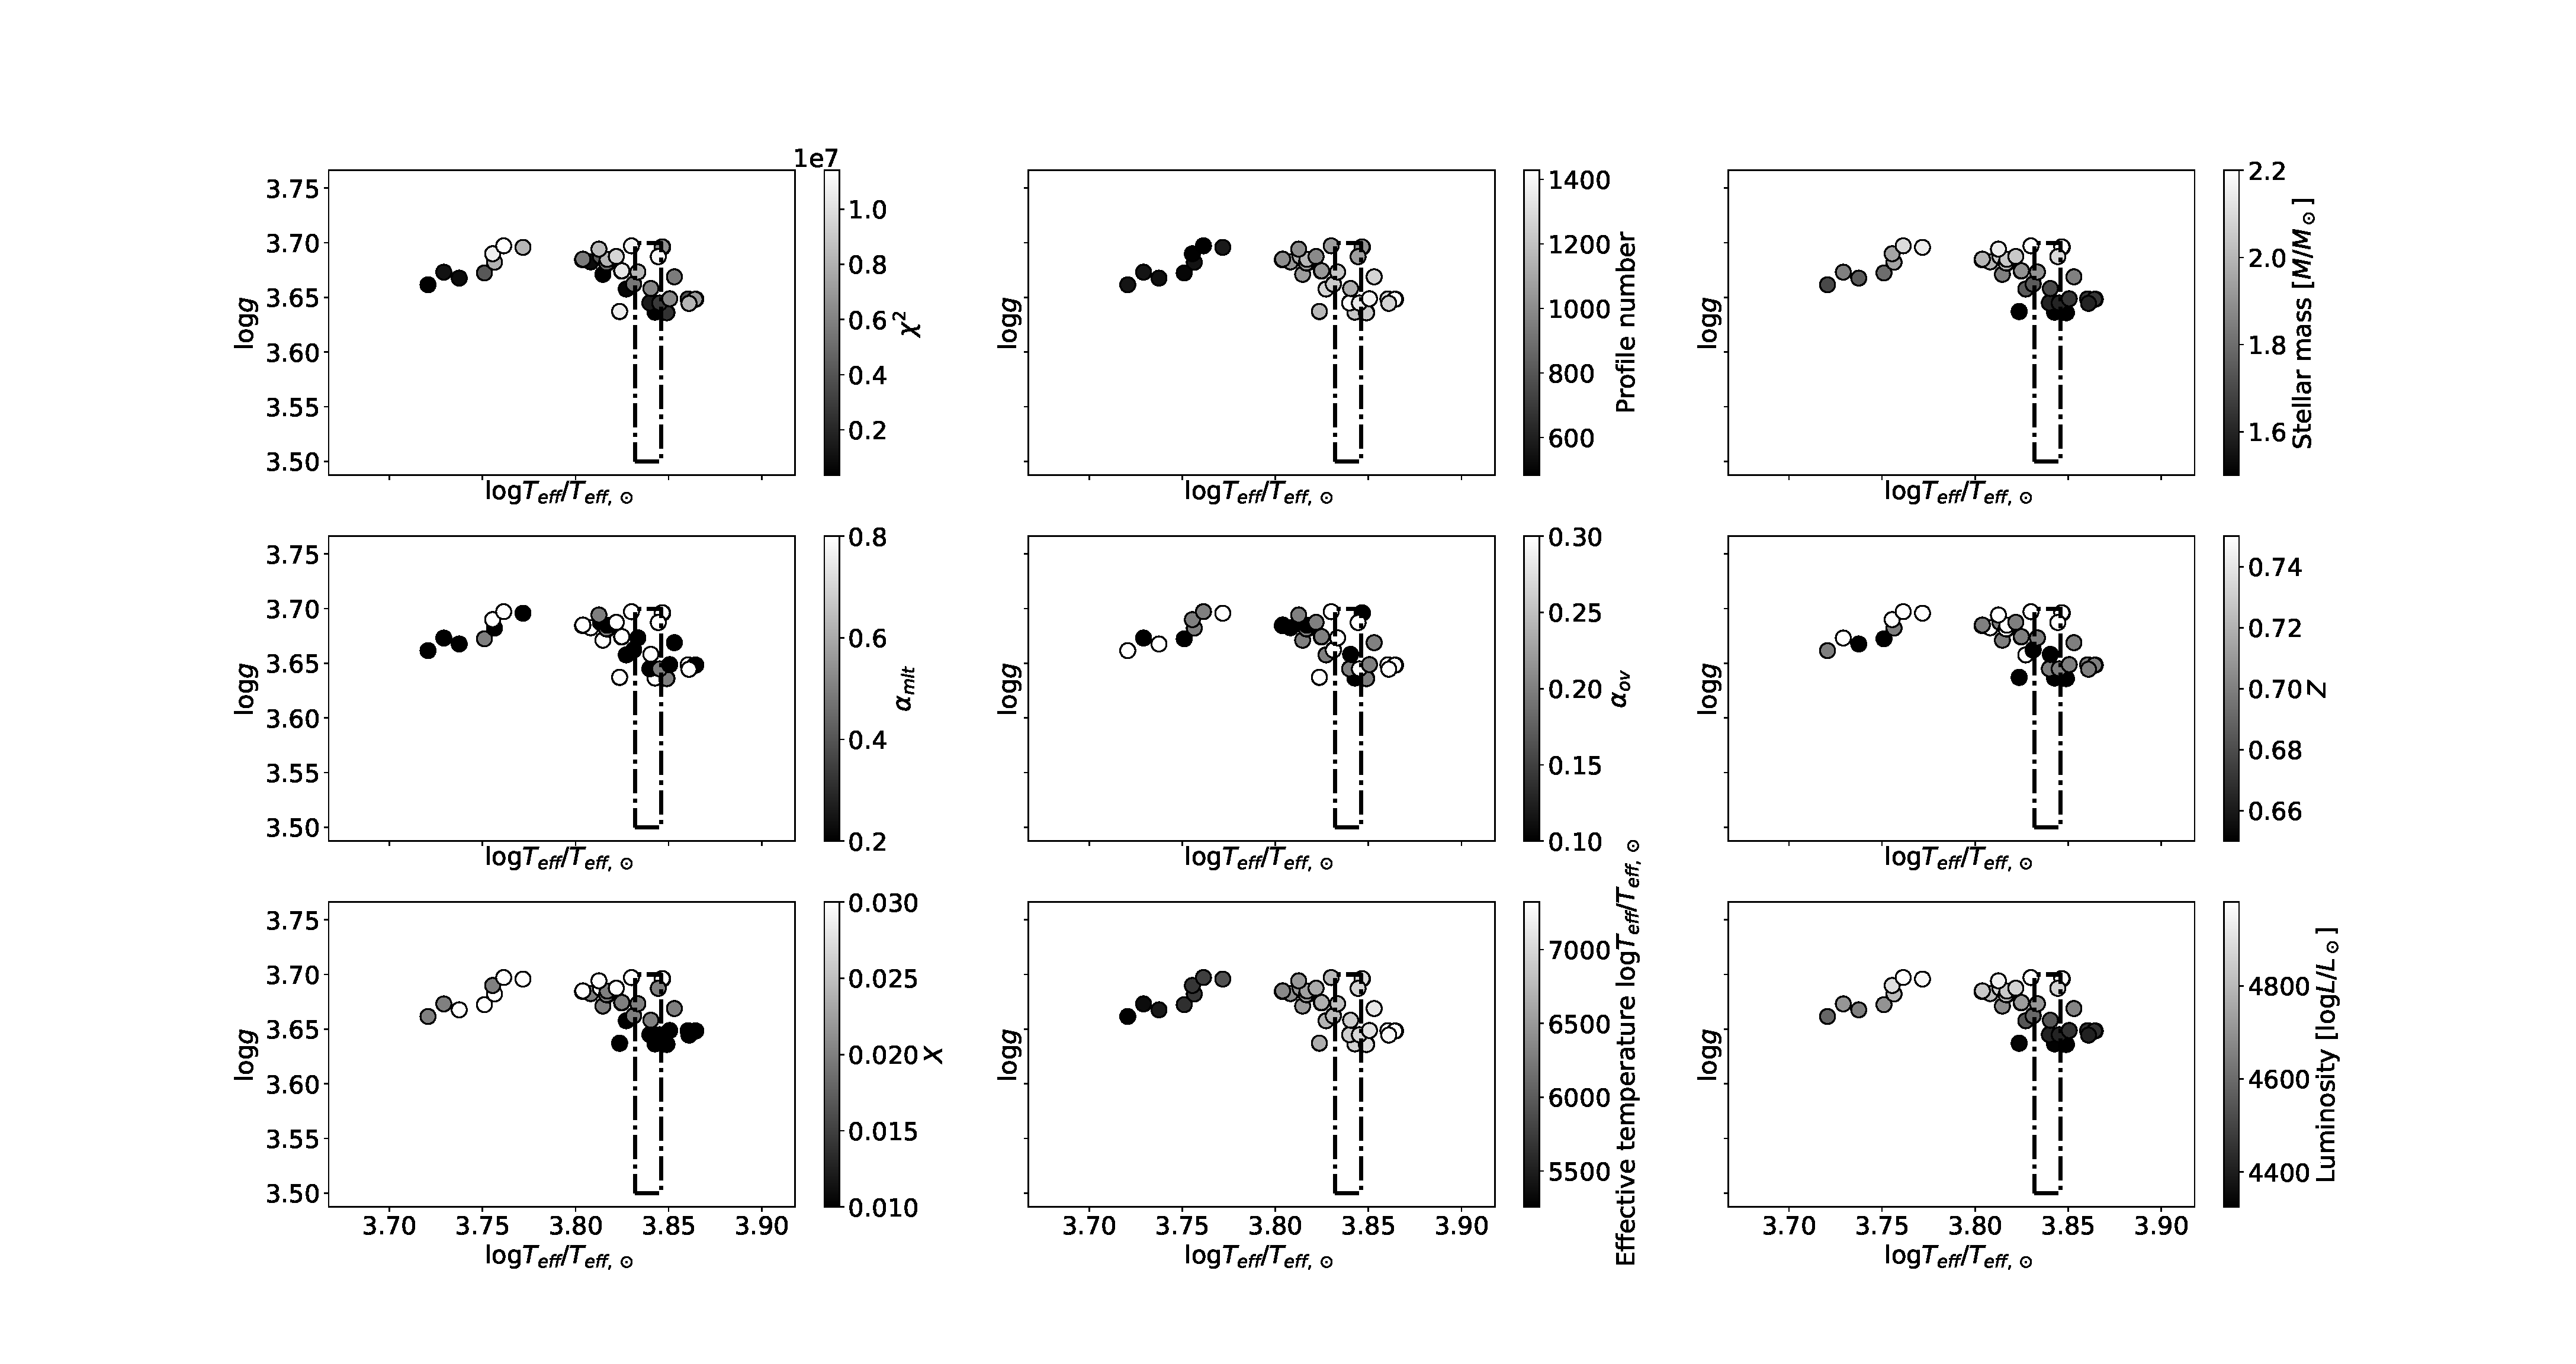
\includegraphics[width=1\textwidth]{scatter_all_v2.eps}
	\makebox[\textwidth][c]{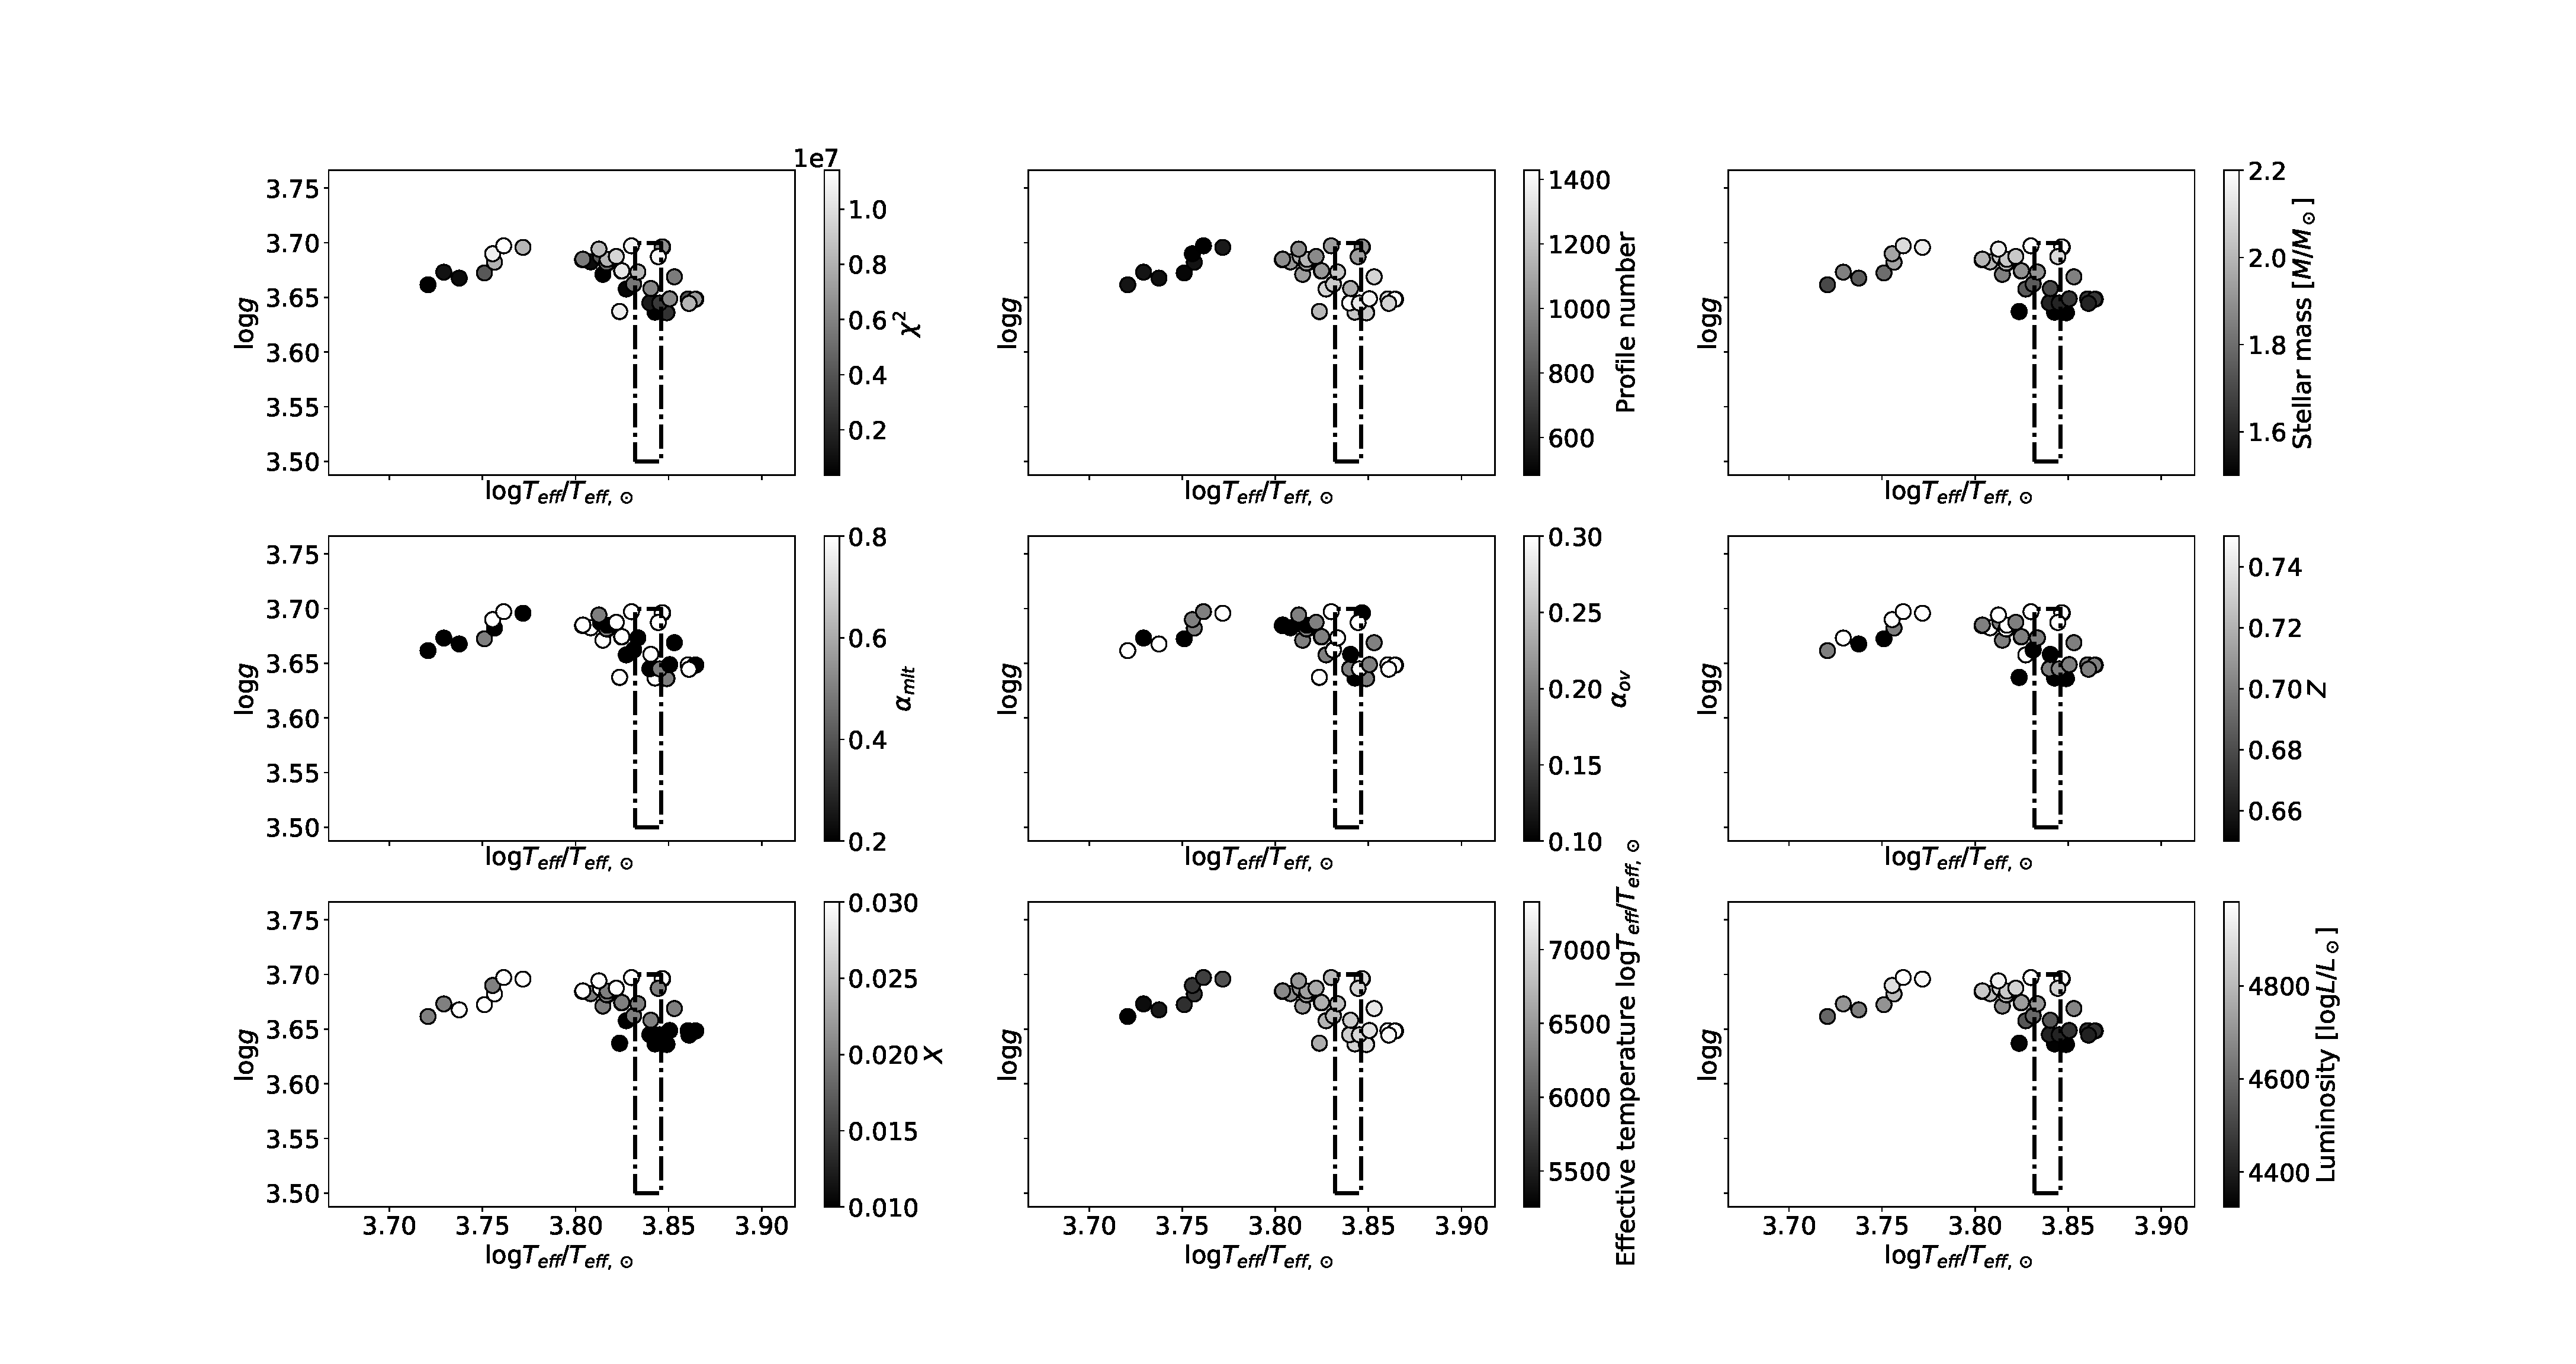
\includegraphics[width=1.5\textwidth]{scatter_all_v2.eps}}%
	\caption{Scatter plots showing \teff, \logg color coded with nine different parameters for the 5\% best models (without resolution control). The plots color coded with \teff and \logg are plotted to show that the plotting method works correctly. The run was made with the Lenz obsevational parameters set. }
	\label{scatter}
\end{figure}


Here, \logg is plotted as a function of \teff and color coded with the corresponding \chis. The 1$\sigma$ uncertainty on \logg and \teff is marked with a black stippled line. Some of the scatter plots shows expected tendencies such as \l, \logg, \teff and profile numbers. Since higher profile number is at a later stage\footnote{Note that the profile number does only indicate the stage of that individual track i.e profile number 900 on one tracks is not necessarily at the same stage for the same profile number on a different track. }, the effective temperature is much lower for lower profile numbers. There is a gap in models around \teff = 3.79 in the 5\% selection criteria. From the profile number it is also clear that the models distributes into two groups where the lower profile numbers corresponds to those on the pre-ms and the higher profile numbers are ms and thereafter. The pre-ms models will be ignored since they are not as reliable as the rest of the models. This group of models is also significantly further away from the errorbox and they will therefore not affect the main result. 

The lowest \chis linearly seems to linearly decrease with \teff. This is because \logg is strongly related to $\rho$ (hence, $\Delta \nu$ and \teff).  
For the element abundances, there is a trend a that lower values of \logg yield lower values of Z and X, in particular. This falls out of \eqref{meanmol} as high abundances of hydrogen and/or metallicity causes a lower mean molecular weight. Since $\mu \propto \rho \propto g$, a smaller value of X or Z yields a smaller value for g as well. Since $g$ is also directly proportional to the mass, the mass decreases with \logg in the plot as well. 

There seems to be no recognizable  in the $\alpha_{mlt}$ and $\alpha_{ov}$ color coding. Since there is a definite correlation between the convection and structure of the star, it would be expected to see a trend between the mixing length or overshoot parameter and \logg and \teff. Since this sample is small, it cannot be excluded that there is a trend that can be found if mode data points were included.   


\subsubsection{l=0,1,2 modes}
A new calculation was conducted in GYRE for l=0, l=1 and l=2 modes for all of these models. The frequencies produced gives a further constrain of the best models as all frequencies can now be compared with observations. Since mode identification is not complete for 44 Tau the radial n,l,m for the frequencies are not finally determined. Therefore they cannot be compared to the individual frequencies calculated in the model without first giving an estimated guess on the n,l and m. Therefore a calculation is conducted based on the fact that n,l and m is known for the models. To ensure that the \chis are comparable between each model, as mentioned earlier, the models all need to have the same amount of fitting parameters. This is not an issue in the first \chis calculations with l=0, since the initial \chis is only based on the same two frequencies for all models. But for l=1 and l=2 the picture is less simple as the number of fitting parameters may vary from model to model, unless it is taken into consideration. The first way to do so is to weight each frequency individually and take the likelihood into account. Though this method probably provides a more detailed and statistically stringent result, it is does require a  very thorough estimate and evaluation of the single frequencies. This is beyond the scope of this work, and instead it is therefore made sure in the way the code is constructed, that this can only be an issue if the number of theoretically produced frequencies is lower than the observed number 8and this is unlikely to happen as these models have already been sorted out in the first \chis round. 

It is carried out in the following way: for each model, each individual model-frequency is compared to all observed frequencies and the best match (i.e. the smallest difference) is thereby assumed to be the closest frequency. This is repeated from the lowest to highest frequency until all model-frequencies has been given a best match observation frequency. This means that the observed frequency will be given the n.l and m of the best -matching model-frequency. Each model then has an estimated set of frequencies where \chis can be computed. This off course does not take into consideration that some frequencies have an estimated radial order and spherical degree. Nor does it take into consideration that the radial fundamental mode and first overtone are already determined (and might match it to n that are higher, however these models should be excluded as their match will not be good if the two first frequencies do not match expectations). This yields a \chis 

\begin{align}
\chi^2 &= \left(\frac{\nu_{\text{all,obs}}^i-\nu^i_{\text{all,theo}}}{\sigma^i_{\text{first}}}\right)^2
 +
         \left(\frac{\text{T}_\text{eff,obs}^i-\text{T}_\text{eff,theo}^i}{\sigma^i_{\text{T}_\text{eff}}}\right)^2  \nonumber \\
  & \quad +
\left(\frac{\log \text{g}_\text{obs}^i-\log \text{g}_\text{theo}^i}{\sigma^i_{\log \text{g}}}\right)^2  + \left(\frac{\log \text{L}_\text{obs}^i-\log \text{L}_\text{theo}^i}{\sigma^i_{\log \text{L}}}\right)^2, 
 \label{eq:chis_all}
\end{align}

From these, the models with the lowest \chis is found for the two different luminosities respectively. . 

\subsection{Results}
The best models found for different runs of 44 Tau are shown in \tabref{bestmodels}. It can here be seen that the variation from GAIA run and Lenz run does not affect the total result. It does however shift the best found model if only including the observational parameters. The reason for this is that the frequencies weigh more in the \chis than the observational parameters. Artificially enhancing the uncertainties on the frequencies does shift the best model, but the total \chis is ...WORSE/BETTER?.

\begin{table}[]
	\begin{tabular}{lllllllllllll}
		profile number & M{[}$M_\odot${]} & X & Z & $\alpha_{mlt}$ & $\alpha_{ov}$ & \textbackslash{}teff & \textbackslash{}logg & \textbackslash{}l & $\chi_{tot}$ & $\chi_{obs_params}$ & $\chi_{freqs}$ & observation set \\
		&                  &   &   &                &               &                      &                      &                   &              &                     &                &                 \\
		&                  &   &   &                &               &                      &                      &                   &              &                     &                &                 \\
		&                  &   &   &                &               &                      &                      &                   &              &                     &                &                 \\
		&                  &   &   &                &               &                      &                      &                   &              &                     &                &                 \\
		&                  &   &   &                &               &                      &                      &                   &              &                     &                &                 \\
		&                  &   &   &                &               &                      &                      &                   &              &                     &                &                 \\
		&                  &   &   &                &               &                      &                      &                   &              &                     &                &                 \\
		&                  &   &   &                &               &                      &                      &                   &              &                     &                &                 \\
		&                  &   &   &                &               &                      &                      &                   &              &                     &                &                 \\
		&                  &   &   &                &               &                      &                      &                   &              &                     &                &                 \\
		&                  &   &   &                &               &                      &                      &                   &              &                     &                &                 \\
		&                  &   &   &                &               &                      &                      &                   &              &                     &                &                 \\
		&                  &   &   &                &               &                      &                      &                   &              &                     &                &                 \\
		&                  &   &   &                &               &                      &                      &                   &              &                     &                &                 \\
		&                  &   &   &                &               &                      &                      &                   &              &                     &                &                 \\
		&                  &   &   &                &               &                      &                      &                   &              &                     &                &                 \\
		&                  &   &   &                &               &                      &                      &                   &              &                     &                &                 \\
		&                  &   &   &                &               &                      &                      &                   &              &                     &                &                 \\
		&                  &   &   &                &               &                      &                      &                   &              &                     &                &                 \\
		&                  &   &   &                &               &                      &                      &                   &              &                     &                &                 \\
		&                  &   &   &                &               &                      &                      &                   &              &                     &                &                 \\
		&                  &   &   &                &               &                      &                      &                   &              &                     &                &                 \\
		&                  &   &   &                &               &                      &                      &                   &              &                     &                &                 \\
		&                  &   &   &                &               &                      &                      &                   &              &                     &                &                 \\
		&                  &   &   &                &               &                      &                      &                   &              &                     &                &                 \\
		&                  &   &   &                &               &                      &                      &                   &              &                     &                &                 \\
		&                  &   &   &                &               &                      &                      &                   &              &                     &                &                 \\
		&                  &   &   &                &               &                      &                      &                   &              &                     &                &                 \\
		&                  &   &   &                &               &                      &                      &                   &              &                     &                &                 \\
		&                  &   &   &                &               &                      &                      &                   &              &                     &                &                 \\
		&                  &   &   &                &               &                      &                      &                   &              &                     &                &                 \\
		&                  &   &   &                &               &                      &                      &                   &              &                     &                &                 \\
		&                  &   &   &                &               &                      &                      &                   &              &                     &                &                 \\
		&                  &   &   &                &               &                      &                      &                   &              &                     &                &                 \\
		&                  &   &   &                &               &                      &                      &                   &              &                     &                &                 \\
		&                  &   &   &                &               &                      &                      &                   &              &                     &                &                 \\
		&                  &   &   &                &               &                      &                      &                   &              &                     &                &                 \\
		&                  &   &   &                &               &                      &                      &                   &              &                     &                &                 \\
		&                  &   &   &                &               &                      &                      &                   &              &                     &                &                 \\
		&                  &   &   &                &               &                      &                      &                   &              &                     &                &                 \\
		&                  &   &   &                &               &                      &                      &                   &              &                     &                &                 \\
		&                  &   &   &                &               &                      &                      &                   &              &                     &                &                 \\
		&                  &   &   &                &               &                      &                      &                   &              &                     &                &                 \\
		&                  &   &   &                &               &                      &                      &                   &              &                     &                &                 \\
		&                  &   &   &                &               &                      &                      &                   &              &                     &                &                 \\
		&                  &   &   &                &               &                      &                      &                   &              &                     &                &                 \\
		&                  &   &   &                &               &                      &                      &                   &              &                     &                &                 \\
		&                  &   &   &                &               &                      &                      &                   &              &                     &                &                 \\
		&                  &   &   &                &               &                      &                      &                   &              &                     &                &                
	\end{tabular}
	\caption{text}
	\label{bestmodels}
\end{table}
The best model results for the Lenz parameter run can be seen on \figref{hrd44taulenz}. The hrd shows the tracks for masses $M = 1.5,1.6,1.7,1.8,1.9,2.0,2.0$ with the combination of $X$ = $Z=$, $\alpha_{mlt}$, $\alpha_{ov}$. The best total model is marked with a cyan blue dot, on the track marked with red. The green points shows the best 5\% models if the criteria is the total \chis\footnote{The total \chis is the \chis from all frequencies, including $l=1$ and $l=2$ modes plus the \chis from observational parameters.}. Blue dots are the 5\% best models if only observational parameters \logg, \teff, \l is included in the \chis, whereas the red dots is the 5\% if the \chis is only calculated from the frequency fits. The green tracks shows the best track with the black dot marking the best model if the frequency uncertainties have been artificially enhanced as in \eqref{sigma}. This track has the parameter combination of $M = 1.5,1.6,1.7,1.8,1.9,2.0,2.0$ with the combination of $X$ = $Z=$, $\alpha_{mlt}$, $\alpha_{ov}$. 

The green points tend to overlap the red points, which indicates that the frequencies are highly more weighted than the observational parameters. The frequencies thereby controls the final outcome, explaining why there is no difference in the main result by changing between GAIA or Lenz observations. The best 5\% models from frequencies seems to be divided into two groups whereas the group near lower temperatures are models on the pre-ms. Since the pre-ms models were loaded from pre-calculated models as discussed in \chapref{compute}, causing different relaxation of the models, the pre-ms and particularly the frequencies on the pre-ms should not be trusted. Since the best model is between the other group it does not make a difference for the main result, but if further tests should be done with the 5\%, they should be excluded from the sample. 

The best model is placing 44 Tau on the post-ms shortly after hydrogen exhaustion in the core. It is not within the three-sigma errorbars from the observations (whereas the best model with artificially pumped frequencies is), which is also clear since there are other models that are closer to the observed parameters. However, since the frequencies weigh much more, the overall \chis is lower. The frequency fit can be seen on \figref{freqfit}. Here, the observational frequencies are plotted with dimensionless power on the y-axis. They color-coded are color-coded by the spherical degree as follows: $l=0$ are red, $l=1$ are blue and  $l=2$ are green, with dimensionless powers of 1,2 and 3. The black lines indicate the matched theoretical frequency, and the gray lines at the bottom represents all theoretically produced frequencies. The naming of the frequencies are defined as in \tabref{freqs44tau}. Stippled lines are lines of uncertainty on the frequencies, although these are so small that they are not visible. Since the uncertainty is so small, technically none of the theoretical frequencies are matched within the uncertainties. However, they are all matched within a range of $0.2 d^{-1}$. The red named text are two modes for which mode identification differs from the theoretically predicted with the \chis fitting code for the frequencies. This is for $f_10$ and $f_2$ where the estimated modes from mode identification is $l=2$ and $l=1$, whereas they were here estimated to be $l=1$ and $l=2$, respectively. This could be due to different reasons: 1) The pulsation code does not calculated the theoretically produced frequencies correctly. At this point it is already a well-known issue that the theory behind these type of oscillations does not comply well with observations. \citet{lenz2010delta} was indeed successfull with modeling 44 Tau, but this example is the first one of its kind where all modes where reproduced theoretically. More often, pulsation codes does not match observations. 
2)  The \chis routine used in this project does not match the frequencies correctly, resulting in the spherical degrees to be found incorrectly. As discussed earlier in this chapter, the routine only considers the best match frequency, and does not take spherical degree into account at any point. It only guesses it based on the theoretically produced ones. 
3) Due to the high uncertainty in mode identification, some of the modes have been done incorrectly. This is the more likely scenario since 1) and 2) would probably cause issues for more than two modes, and would not have been able to fit the rest either. There is also strong evidence that some modes could be identified wrongly due to the model dependency of the mode identification. It can be seen on \figref{lenzdiss} that the choice of mixing length affects the mode identification significantly. EXPLAIN FIGURE. These models are based on frozen convection where the mixing length describes the local convection. However, time-dependent convection is needed in order to describe the full picture of convection, and the difference in mode identification is significant \citep{dupret2005time}, (Victoria Antoci 2019, private communication).

\begin{figure}[htbp]
	\centering
	%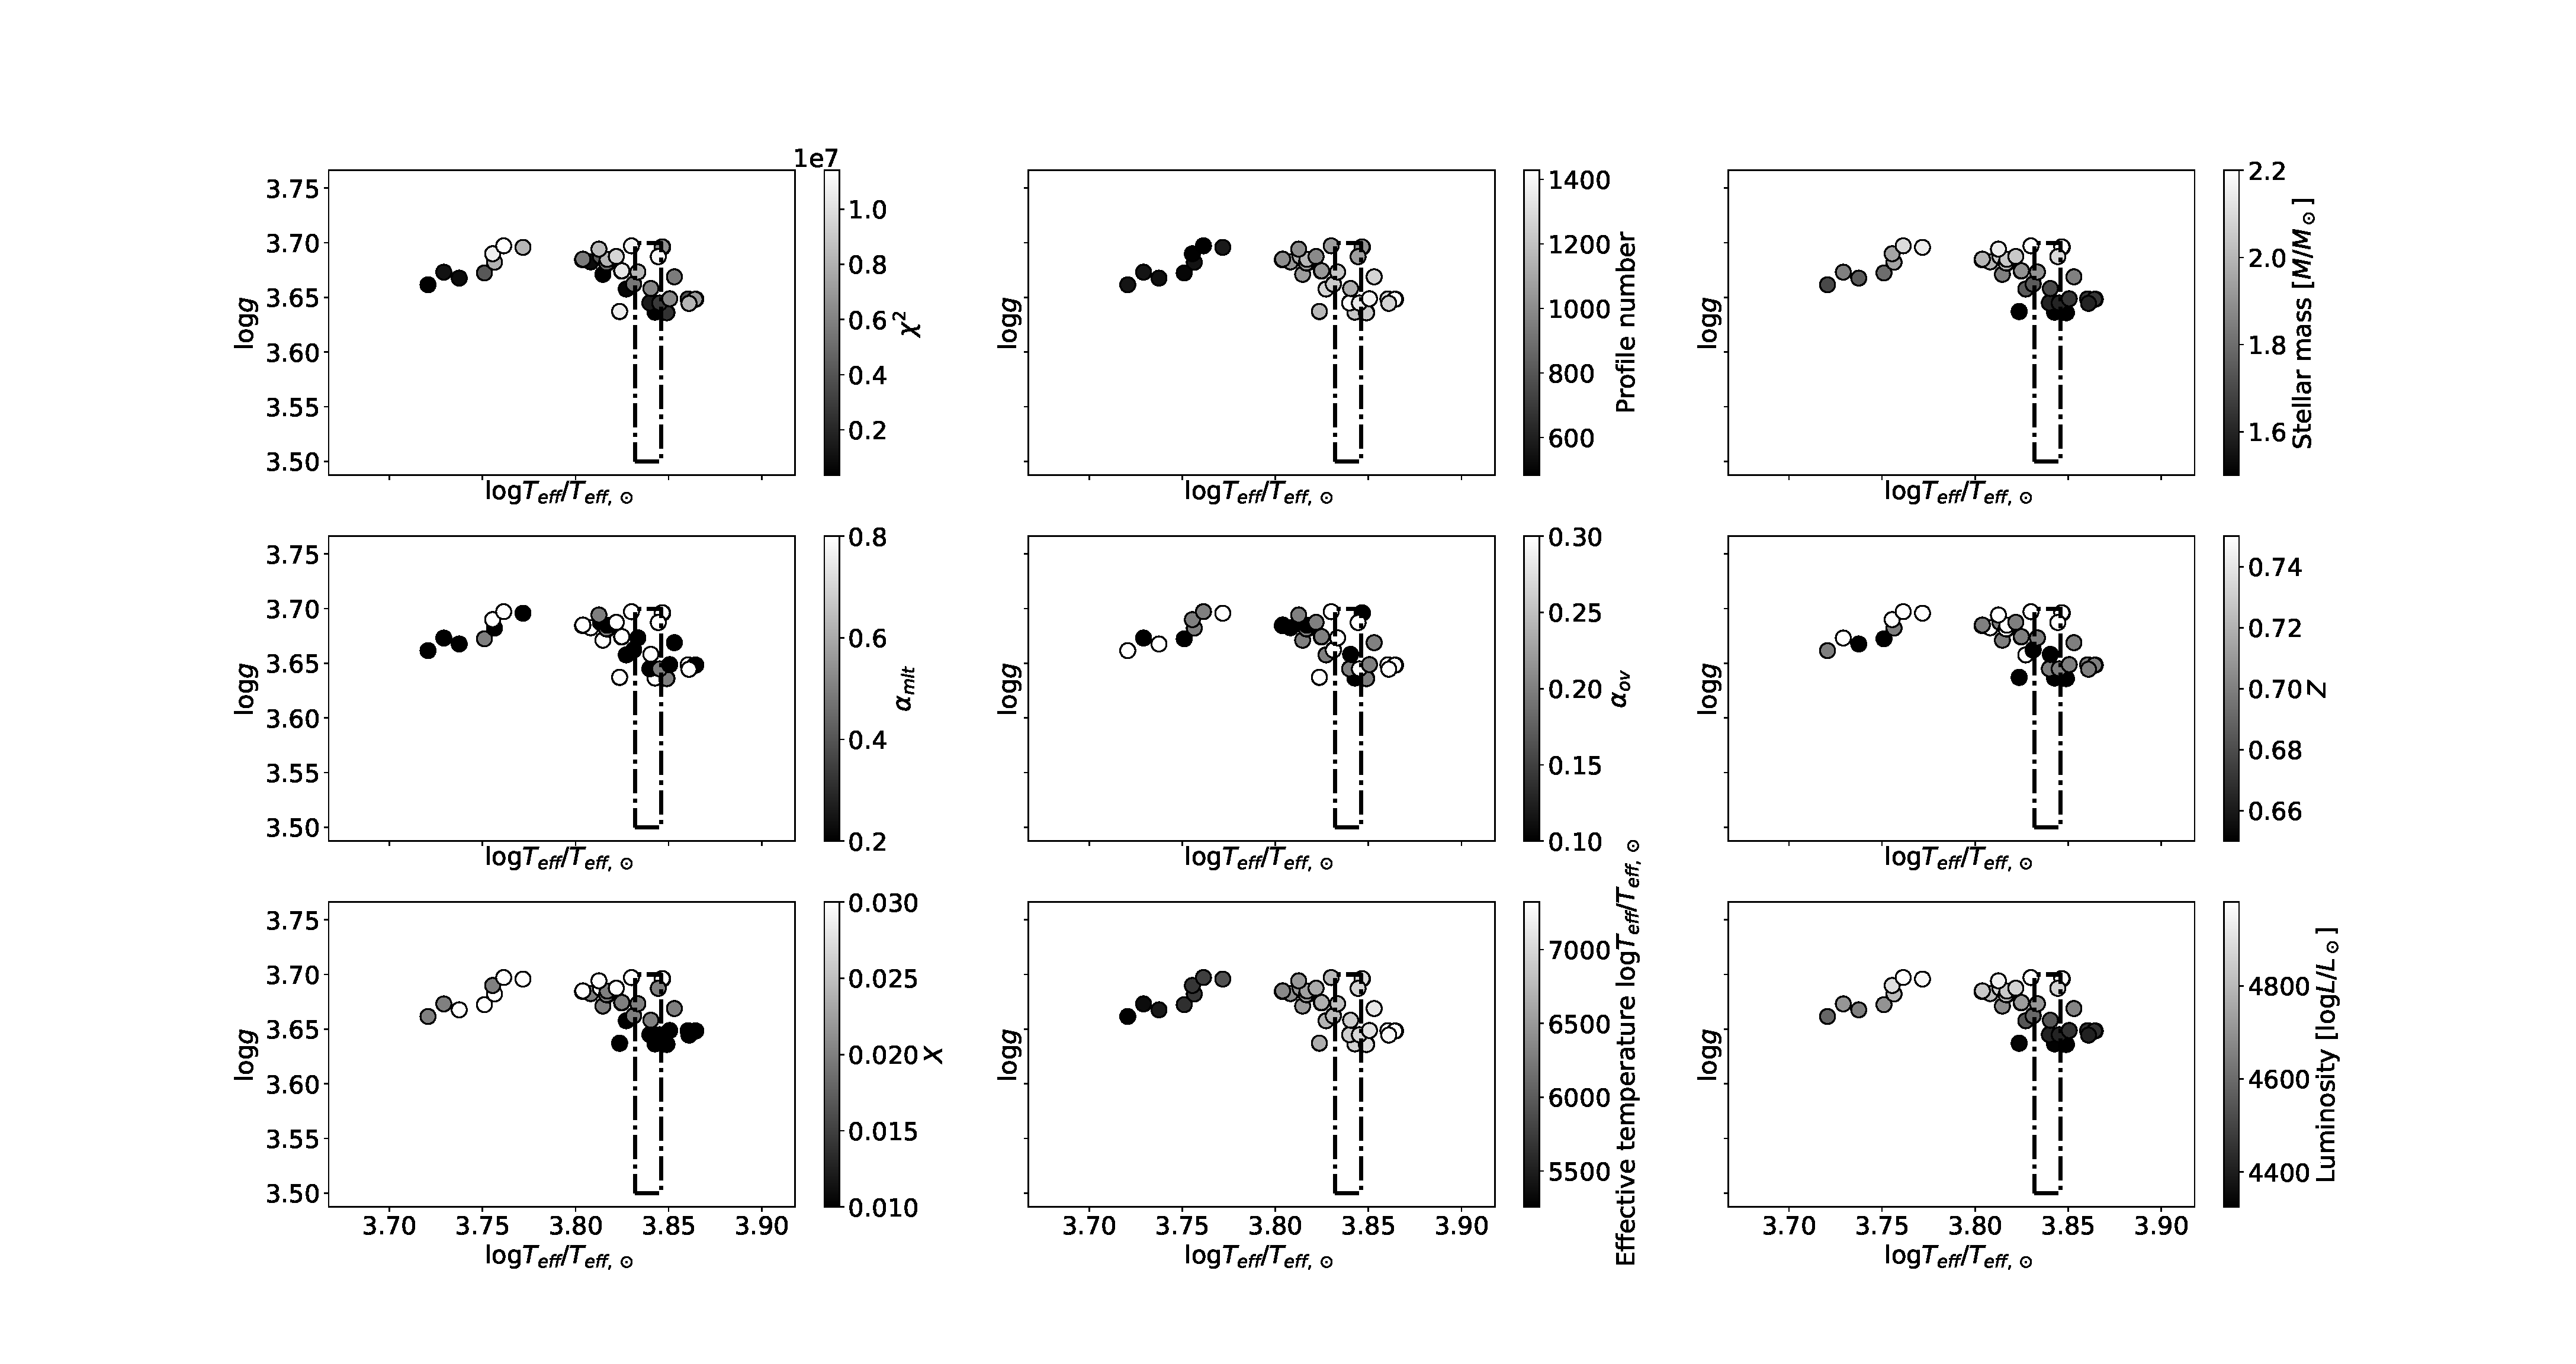
\includegraphics[width=1\textwidth]{scatter_all_v2.eps}
	\makebox[\textwidth][c]{\includegraphics[width=1.5\textwidth]{final_hrd_44tau_lum1.eps}}%
	\caption{}
	\label{hrd44taulenz}
\end{figure}

\begin{figure}[htbp]
	\centering
	%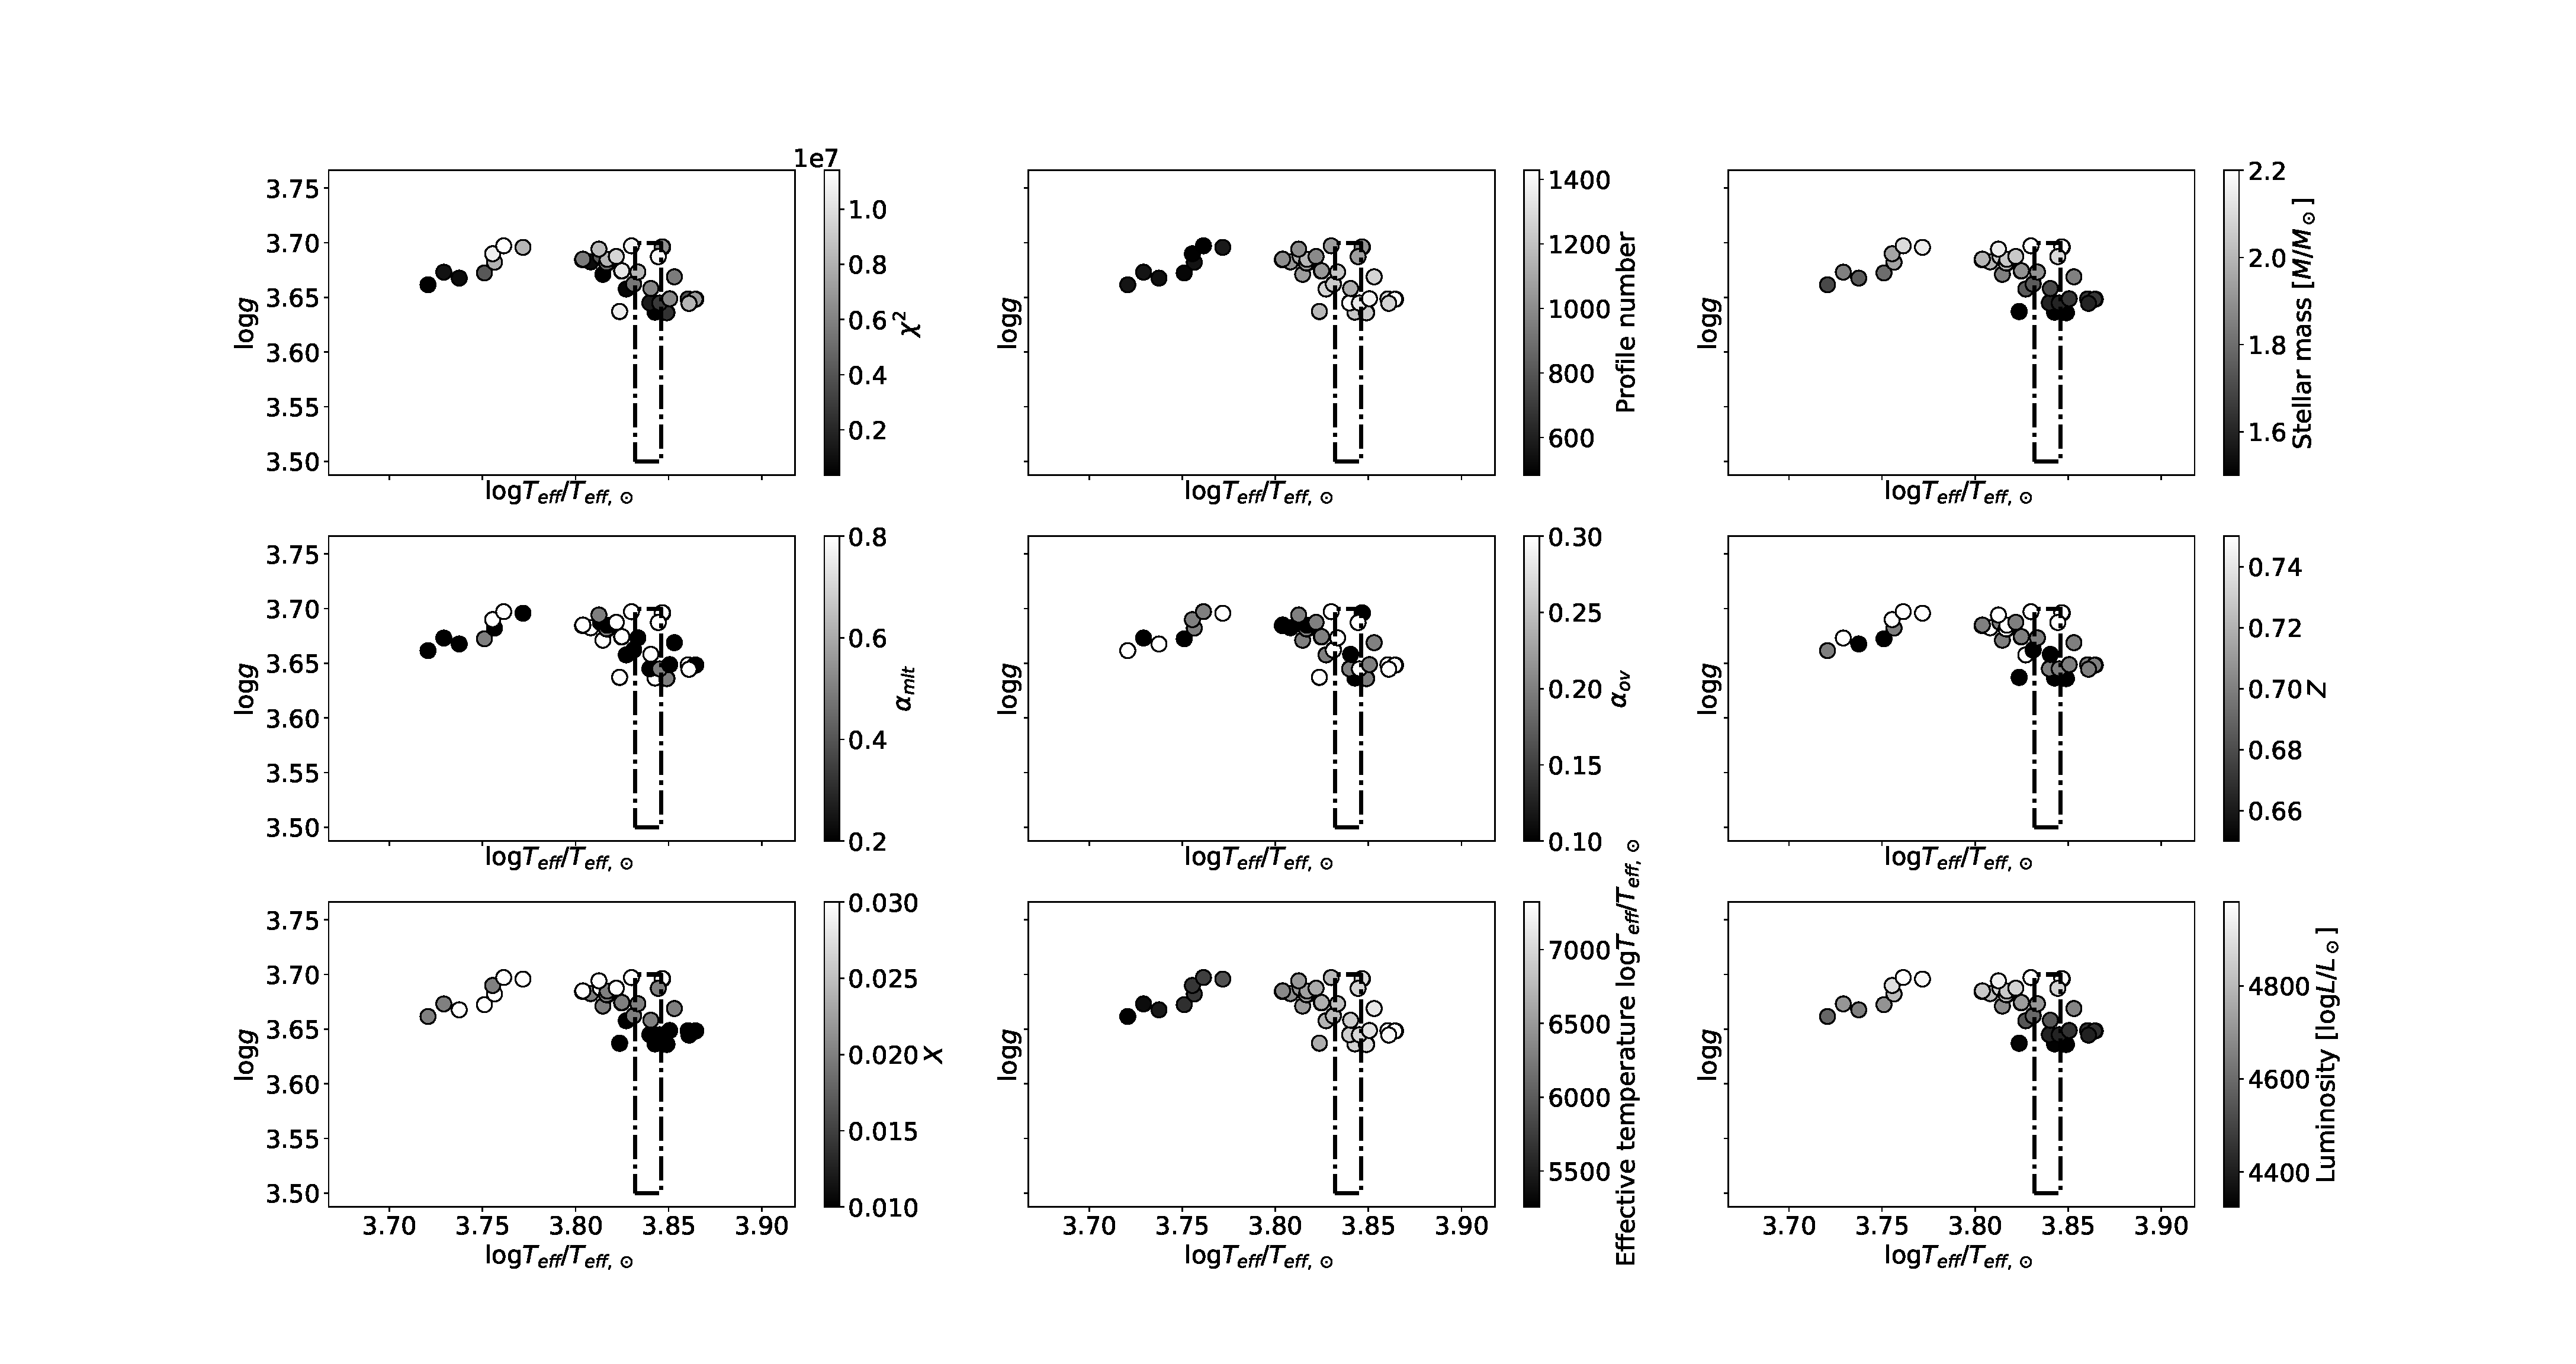
\includegraphics[width=1\textwidth]{scatter_all_v2.eps}
	\makebox[\textwidth][c]{\includegraphics[width=1.5\textwidth]{frequency_fit.eps}}%
	\caption{}
	\label{freqfit}
\end{figure}

\section{Superstar}

On the contrary to 44 Tau, no modes are well enough determined to use an initial constraint for the models of this star. Instead of fitting the frequencies it is therefore more favourable to fit the large frequency separation, introduced in \secref{chap:asteroseismology}. This can be calculated as

\begin{equation}
    \Delta\nu = \nu_{n+1} - \nu_{n},
\end{equation}

\noindent the frequency difference between two (l=0).  The \chis can now be calculated using the observed large frequency separation of 3.5 cycles per day \citep{antoci2014role}, calculated the same way as  \eqref{sigma}, with method one \eqref{sigma}. Employing the standard deviation as \eqref{m2} cannot be done the same way as for 44 Tau since there is only one parameter to sum over. Therefore, the 5\% models with the smallest \chis are found only through the first method, and results are shown shown in \tabref{tab:superstar}.

\begin{table}[htbp]
  \caption{hest}
  \label{tab:superstar}

\begin{tabular}{lllllllllll}
\label{bestchi}
 Model & X & Z & Y & $M[M_\odot]$ & $\alpha_{mlt}$ & $\alpha_{ov}$ & $\log \text{T}_\text{eff}$  & $\log \text{L}$  & $\log \text{g}$ & $\chi^2$ \\
 &  &  &  &  &  &  &  &  &  &  \\
 &  &  &  &  &  &  &  &  &  &  \\
 &  &  &  &  &  &  &  &  &  &  \\
 &  &  &  &  &  &  &  &  &  &  \\
 &  &  &  &  &  &  &  &  &  &  \\
 &  &  &  &  &  &  &  &  &  &  \\
 &  &  &  &  &  &  &  &  &  &  \\
 &  &  &  &  &  &  &  &  &  &  \\
 &  &  &  &  &  &  &  &  &  &  \\
 &  &  &  &  &  &  &  &  &  &  \\
 &  &  &  &  &  &  &  &  &  &  \\
 &  &  &  &  &  &  &  &  &  &  \\
 &  &  &  &  &  &  &  &  &  &  \\
 &  &  &  &  &  &  &  &  &  &  \\
 &  &  &  &  &  &  &  &  &  &  \\
 &  &  &  &  &  &  &  &  &  &  \\
 &  &  &  &  &  &  &  &  &  &  \\
 &  &  &  &  &  &  &  &  &  &  \\
 &  &  &  &  &  &  &  &  &  &  \\
 &  &  &  &  &  &  &  &  &  &  \\
 &  &  &  &  &  &  &  &  &  &  \\
 &  &  &  &  &  &  &  &  &  &  \\
 &  &  &  &  &  &  &  &  &  &  \\
 &  &  &  &  &  &  &  &  &  &  \\
 &  &  &  &  &  &  &  &  &  &  \\
 &  &  &  &  &  &  &  &  &  &  \\
 &  &  &  &  &  &  &  &  &  &  \\
 &  &  &  &  &  &  &  &  &  & 
\end{tabular}
\end{table}

For modes higher than l=0, calculating the \chis for Superstar is significantly more complicated for Superstar, since it is based on the large frequency separation. When l becomes larger than zero, the frequency separation depends significantly on the mixed modes and radial order. Therefore, this part is beyond the scope of this work. 

\subsection{Results}
If HD 187547 is indeed on the pre-me we would expect features from different metallic lines and dust to appear in the spectrum, however no so observations indicate that this should be the case. As mentioned, the pre-ms tracks in \texttt{MESA} made in this work should not be trusted for  the purpose of asteroseismic modeling, since the are all products of the same relaxed pre-calculated pre-ms model. Therefore, the results are forced on to the ms by making a cutoff at profile 900. This is a rough cutoff since profile 900 on one tracks is not necessarily an indication of the same stage for the same profile on another track. A more secure way do it would be to evaluate the helium content in the core and set a limit for the gradient (i.e. defining the ms at a certain limit for an increase in helium in the core). This would however require an individual assessment of each track, and is therefore beyond the scope of this work. 

The issues with modeling HD 187547 compared to 44 Tau are still very much up for discussion. The very small luminosity measured observationally could be explained if it is still in a vary early stage on the ms. Then we would expect $\delta \nu$ to be significantly larger than $3.5d^(-1)$, more like $7d^(-1)$ from Bedding. However, since the pre-ms tracks made in \texttt{MESA} in this work are not made for modeling purposes, the earlier stages of the ms might be affected as well (due to relaxation issues etc.). For the small frequency separation, the results seems more reliable as the 5\% best models for separation and observations has some overlap, which is not the case for the $\delta \nu = 7$. This could be due to several things: 1) The models are simply not trustworthy at these early stages due to insufficient pre-ms tracks. 2) From the resolution evaluation discussed in \secref{sec:resolution}, it was shown that models have smaller resolution at the early stages. If HD 187547 is indeed at a very early stage on the ms, the models are very far apart at this point, causing a larger gap between models. This does not however explain why there is a missing overlap between separation selected models and observation selected models.
3) More constraints are needed on the frequency calculations. As was shown in \chapref{introduction}, the asymptotic relation is only applicable to $n >> l$. This affects the large frequency separation, since the equidistancy in frequency space is otherwise invalid. The frequencies were calculated in the range of $45d^(-1)$ to $80d^(-1)$ to somewhat avoid this issue. But for younger models the frequency of $45d^(-1)$ might still be at very low radial orders $n$(since younger models have higher frequencies), which causes a bias in the models. A plot of the theoretically produced fundamental mode as a function of evolution is shown on \figref{fundmode}.  The equidistancy is valid only for the part of the plot that is a straight line. This covers a frequency range of .... which is good/bad because....


%\begin{figure}[htbp]
%	\centering
%	%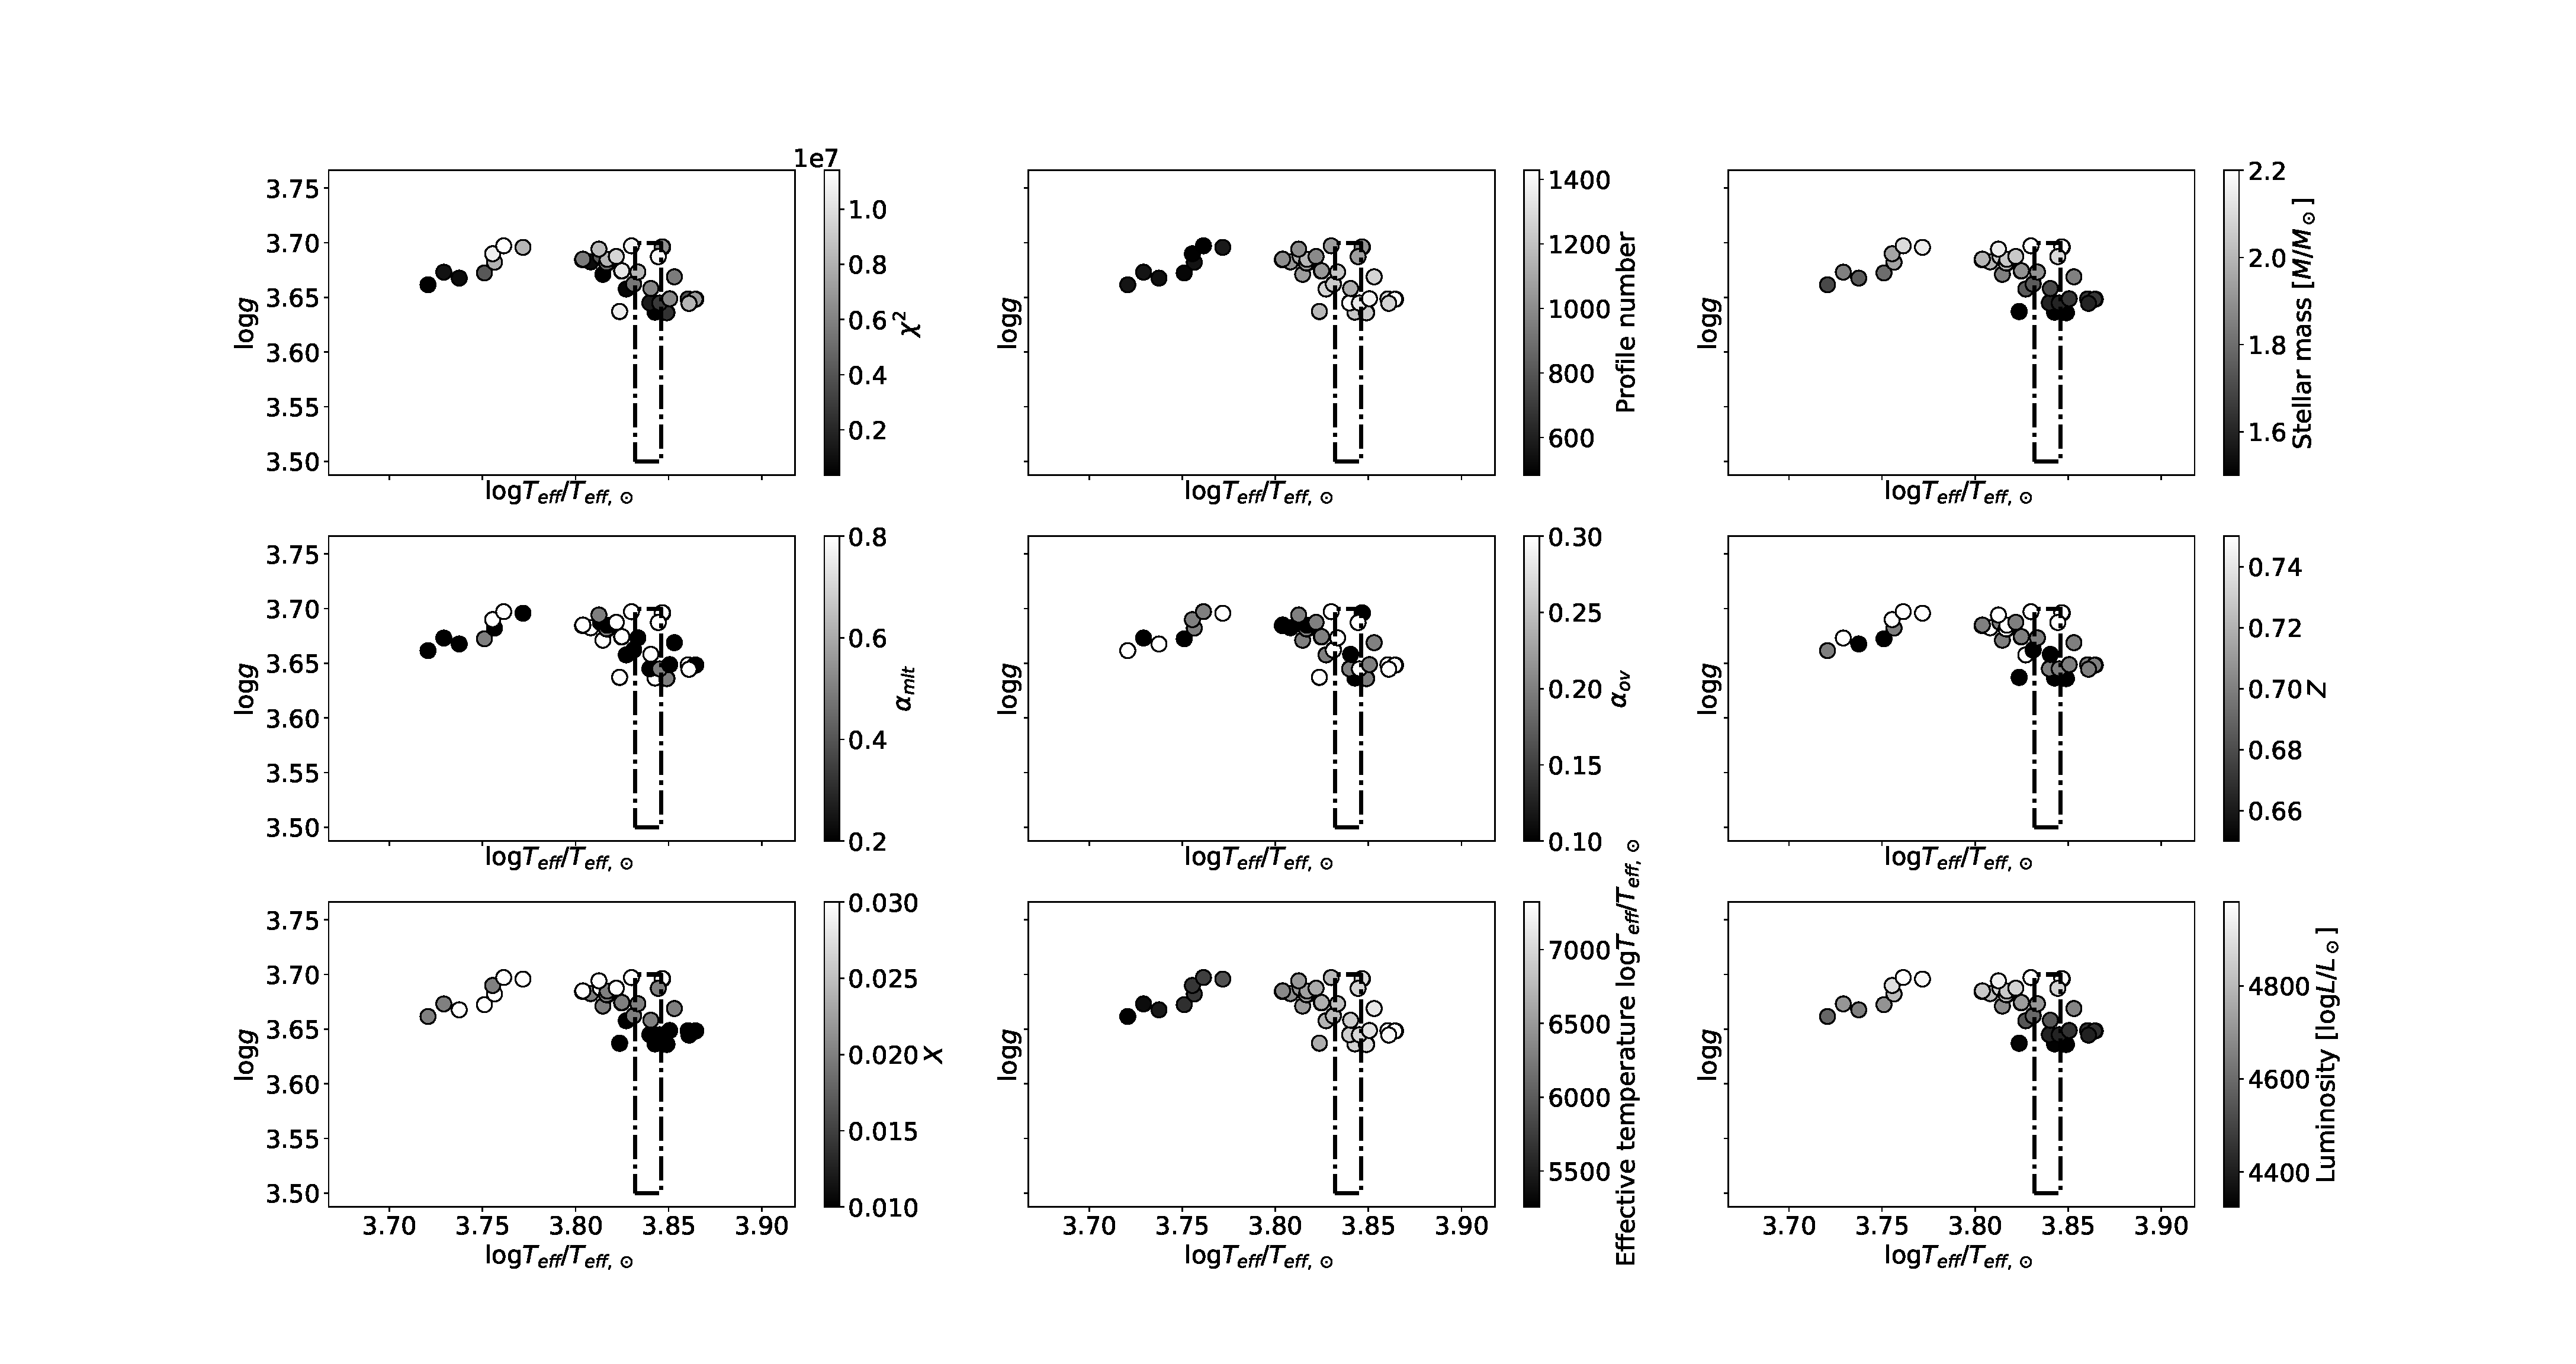
\includegraphics[width=1\textwidth]{scatter_all_v2.eps}
%	\makebox[\textwidth][c]{\includegraphics[width=1.5\textwidth]{frequency_fit.eps}}%
%	\caption{}
%	\label{}
%\end{figure}
\chapter{Discussion and future work}
\label{sec:discussion}

In this chapter the results will be discussed in more detail for the purpose of proposing any issues and aspects that needs to be addressed in future work for obtaining further knowledge and improvement. 

Discussion points, and future stuff:

\begin{itemize}
    \item Testing opacities and element abundances
    \item Rotation in models (both mesa and GYRE)
    \item Further analysis of mlt and overshoot in particular - different prescriptions
    \item a few models could simply not be converted
    \item a more thorough analysis on the grid and which models work
    \item Additional varcontrol!
    \item non-adiabatic treatment and excited frequency range
    \item further mass analysis with petersen diagrams

\section{Grid considerations}

The grid of tracks constructed for this project proves sufficient for providing an estimate on the range in the evolutionary stage for 44 Tau and HD 187547. It stretches from a mass of 1.5 to 2.2 \msun to cover up most of the instability strip in the parameters space. However, as $\delta$ Sct pulsators have been observed even outside of the instability strip, it is important to include that possibility of more extreme parameter space possibilities. Therefore, further analysis in the future should include a more detailed evaluation of the outer grid bounds to analyse the probability of the best fit models in those ranges. As the mass boundary for $\kappa$ mechanism is still an ongoing discussion (reference), a larger grid including masses up to 2.5 \msun should be included in the grid to ensure full coverage. 
Since $\alpha_{mlt}$ is a purely empirical parameter and therefore not directly applicable in analytical solutions, there are not many guidelines as how to the range in the grid should be chosen. Here, smaller values were initially chosen due to two reasons: Firstly, the values for $\alpha_{mlt}$ in \citep{lenz2010delta} is as low as $\alpha_{mlt}$ = 0. Hence, the values in this project must be correspondingly small in order to compare results more easily. However, this argument becomes faulty as soon as the implementations of $\alpha$ mlt is not the same in both stellar structure and evolution codes, meaning that the same number has different interpretations. Although, secondly, one might still argue that such small values still is a good estimate for stars with very small convective envelopes, since the convection is not efficient. This is very much still up to discussion, since convective efficiency and how it affects the excited frequencies, despite efforts (references), still lacks understanding. For this project, the effects of different mixing lenght throughout the HRD is shown on \figref{mlt}, and as earlier discussed in \secref{compute} it primarily has affects the star in the late stage of the subgiant phase.  However, the effects it will have on the frequencies is more vast, as can be seen on ...

From this it is clear that the structure changes that follows from different choice of mixing lengths affects the frequencies quite vastly, pushing them to (higher of lower) which could result in a bias in the best 5\%, pushing the best model results towards (lower, higher values of logg?). For future work, it would therefore be worthwhile to extend the $\alpha_{mlt}$ to values as high as the standard solar value of 1.8 in \texttt{MESA}. This ensures the exclusion of unconscious bias from the grid  choice. 
 
As mentioned in \secref{sec:chi44}, the uncertainties of the frequencies are very small, causing the values of the total \chis is completely controlled by the frequencies. A method taking the resolution into consideration was implemented through \eqref{function}. It was also showed that this made no significant difference to the best 5\%, as the \chis values for the frequencies is still significantly higher than for the rest of the parameters. This proves that the resolution is not troublesome enough to cause a change of the best model. (is it though?). It can also be argued that frequencies should naturally be weighed higher as the observations have smaller uncertainties, and that the \logg, \teff, and \lum should be given correspondingly smaller weights due to higher uncertainties (and disagreements between spectroscopic and photometric values). This is also done automatically in this project since the \chis is calculated by dividing with the uncertainties. However, this does cause the frequencies to weigh much more than intended, and it would therefore be relevant to conduct an implementation of more thoroughly selected weights for all the fitting parameters. (How would this be doe though?). 

Even though implementing the resolution into the \chis does not change the main results, it is still favorable to have as many points on a track as time allows. As discussed, this is time consuming computationally, but ensures a minimized \chis. The \texttt{target} command in \texttt{MESA} allowed for a somewhat better resolution (particularly for tracks with high $\alpha_{ov}$), but more options to increase the resolution even further should be considered in future work. This analysis was primarily focused on the evolutionary stage of the stars, but also depends strongly on the input parameters for the tracks. In this work, the step size of the tracks is bigger than that of \citet{lenz2010delta}, resulting in a larger difference in parameter space. Thus, models in between these tracks are not considered. Since creating an entire grid is time consuming, doubling it up would take very long, and could prove excessive particularly in those areas of the HRD where it would be less likely to find $\delta$ Sct pulsations. Instead, grid with smaller step sizes could be constructed around the tracks of either the best 5\% models, or those with higher likelihood. The latter is, however, a different statistical approach where each model input parameter gives a likelihood. Both ways would also allow for a more detailed evaluation of the individual model parameters, particularly the $\alpha_{mlt}$ and $\alpha_ov$. By further constructing a narrow but dense grid around the best model, it can be tested if the minimal \chis is still on the original track, or if \chis can be optimized even further.  

%This would also contain more information on not only the best stage estimate, but the parameter combination as well. The general approach used here is     

Throughout this project, the grid constructed was only calculated using gs98 element abundances and OPAL opacities. This was done due to limited time. However, as \citet{lenz2010delta} showed in his asteroseismic modeling of 44 Tau,  the tracks and thereby the evolutionary stage are affected by this choice. Therefore, a further analysis of the choice is needed in order to determine if the best model \chis 


\section{Stringent statistics}

From a statistical point of view, the \chis test carried out in this work is crudely simplified for the purpose of answering the question of which evolutionary stages the stars are in. The \chis is merely a number that gives the sum of differences for the parameters, but a small \chis does not necessarily mean that that model has the highest \textbf{likelihood}. In order to compare \chis between all models in the grid, strictly speaking, the conditions should not change between the models as the individual parameters are then weighted differently. Therefore, since \eqref{sigma} and \eqref{m2} are not weighted the same way as the rest of the parameters, the sum of parameters depends on two different weighting methods (even though the $\alpha$ does somewhat act as a translation between them). This is not a problem in itself, but it is more statistically correct to calculate \chis independantly from the restt of the parameter  This means that comparing the same tracks for a different observed luminosity needs to be done very carefully since the uncertainties of the luminosities are different, and the \chis are thereby automatically weighted differently.

More on if it is actually a problem. 

\end{itemize}
\chapter{Conclusion}
\label{sec:conclusion}

The goal of this project was to use asteroseismic modeling on the two stars 44 Tau and HD 187547 respectively, in order to extract information on their frequencies, stellar parameters and evolutionary stages. For this purpose, a grid of models was calculated with \texttt{MESA} stellar structure and evolution code to simulate their evolutionary tracks. The \texttt{GYRE}  pulsation code calculated theoretical frequencies for the entire grid to simulate the pulsations within the star. The resolution of the tracks were tested and improven to ensure that all stages of the evolution were properly resolved. 

A \chis method was implemented for both stars, in order to fit observed parameters to modeled parameters.  The \chis was implemented as defined by \eqref{sigma}. The uncertainties of the frequencies were artificially enlarged through the resolution in a second \chis implementation for 44 Tau. The purpose of this was to test if the frequencies needed to be weighed less to compensate for the small uncertainties. In both bases, 44 tau was successfully modeled to be on the post-ms. For the classical \chis approach, the best fitted model was on the tracks with mass $M=1.65M_\odot$....... and the best model is on the post-ms, specifically on the Heney hook, shortly before hydrogen exhaustion. For the artificially enhanced case, the resulting best model was better fitted to the observational parameters \teff,\l and \logg with the evolutionary stage being slightly later. However, the matched modes of the frequencies from models differs from the mode identification more than in the classical case. This indicates that there is a trend running counter between model frequencies and observational parameters. It is not clear whether this is due inadequacy of the models (lack of time-dependent convection treatment and non-adiabatic calculations of the frequencies.), or a bias in the grid stemming from the low $\alpha_{mlt}$ values. 
The results of the evolutionary stage confirms the work from \citet{lenz2010delta}, although with a slightly lower mass. Further investigation is needed in order to address the difference between model parameters of this work and \citet{lenz2010delta}. The grid needs to be narrowed down in parameter space, bout have more grid points instead. This should be done around the best model, in order to test if the \chis can be optimized more options for parameter combinations. The low values of $\alpha_{mlt}$ causes a bias in the models as the frequencies are strongly related to the models. Therefore, the grid needs to be tested with standard values around $\alpha_{mlt}=1.8$ also. 

For HD 187547 the modeling was conducted through fitting the theoretically calculated large frequency separation to two different observed estimates \citet{antoci2011excitation} (private communication,Victoria Antoci, Bedding et al. in review). The modeling was limited to $l=0$ modes with a frequency range of $45-80 d^{-1}$ since modeling the larger frequency separations for higher $l$ requires a more advanced routine than implemented here. This was done for $\Delta\nu = 3.5 d^{-1}$ and $\Delta\nu = 7 d^{-1}$ respectively. Results showed that for both $\Delta\nu$, the star is on the ms (although at a younger stage for the highest $\Delta\nu$). The  $\Delta\nu = 3.5 d^{-1}$ best track was outside the borders of the instability strip, and the best models \chis for observed parameters and large frequency separation did not overlap. This strongly indicates that $\Delta\nu = 3.5 d^{-1}$ is too low to account for the low value of \lum, and that the star is indeed at the earlier stages of the ms. A cutoff was made in the grid to exclude models on the pre-ms. Since it is an exact cutoff,  the removal of ms models on some track was unavoidable. It is therefore a possibility that the star is even younger than modeled here. For future work, a cutoff should be made based on the helium content in the core, to find the ms on each individual track. 
The asymptotic relation is valid when the frequencies decrease linearly with evolution, and this range should therefore be evaluated to exclude models where the frequency range does not behave asymptotically. The results will be biased for young models since the radial order can still be very small even for a high frequency. For future work, the models should therefore be constrained to high-order radial modes where the asymptotic relation is valid. Additionally, the high order $l$ should be considered in the calculation of the separation. This could be done by cross-correlation between frequencies for selected model, as this would work for any $l$. 


\printbibliography
\chapter{Appendix}
\section{Inlist files from MESA and GYRE}
\label{inlist}

\subsection{MESA inlist}

The standard inlist file used in \texttt{MESA} grid construction for this work is shown here. The \texttt{initial\_h1},\texttt{initial\_he3},\texttt{initial\_he4}, \texttt{mixing\_length\_alpha}, \texttt{new\_mass} and the different \texttt{step\_overshoot\_f} commands changes the values of $X,Z,M,\alpha_{mlt},\alpha_{ov}$ respectively. This is done through a bash script searching and replacing the correct values. 

\lstinputlisting[language=Fortran]{appendix_stuff/inlist_premainmade}

\subsection{GYRE input file to output}

This section shows a bash script which creates an inlist file to run GYRE on a profiles.data.GYRE output file, and create an output file. This code has the option to call radial orders only.
\lstinputlisting[language=Bash]{appendix_stuff/gyre_tofreqs_44tau.sh}

\section{\chis routine}
\label{chisroutine}

For the purpose of calculating the \chis, multiple codes are used. Here, only some of them are presented. All files used in this project can be seen on the webpage \url{https://github.com/JanneMon/Thesis-codes}. 

First, all profiles for all tracks located in the grid directory (\texttt{output\_smallgrid}) are read into \texttt{call\_chi.py} which is the main file. This calls several files (not listed here) to extract input parameters, observational properties and pulsations.  A file with all the information is created for each track and put into a separate directory \texttt{Results\_l0}\footnote{The "l0" indicates that the luminosity comes from the first dataset}. 

\lstinputlisting[language=python]{appendix_stuff/call_chi.py}

This also does call an initially used \chis code \texttt{calculate\_chis\_ff1.py} which was implemented wrong and resulted in $\chi_{freqs}=1$. Therefore, the correct \chis test used in this project is conducted in a separate file \texttt{call\_chi\_actually} that takes the output files in the \texttt{Results\_l0} directory, calculates the \chis based on the observational and pulsational values in the file and creates a new results file in \texttt{new\_Results\_l0}. 

\lstinputlisting[language=python]{appendix_stuff/call_chi_actually.py}

The output files created contains all \chis information $\chi_{tot}^2$,$\chi_{freqs}^2$, $\chi_{obs}^2$ and the artificially pumped total \chis and frequencies $\chi_{p}^2$, $\chi_{freqs,p}^2$. For each file (containing information for an entire track) the lowest $\chi_{ tot}^2$ is found. Among these, the best 5\% models are found. These selections happens in \texttt{plot\_chis\_actually.py}:

\lstinputlisting[language=python]{appendix_stuff/plot_chis_actually.py}

This will create an ouput file with the names of the 5\% best models, as listed in \tabref{bestchi_m1}. It also produces a plot with the best \chis model for each track plotted as a function of mass. An example plot can be seen on \figref{selectfive}. 

\begin{figure}[htbp]
	\centering
	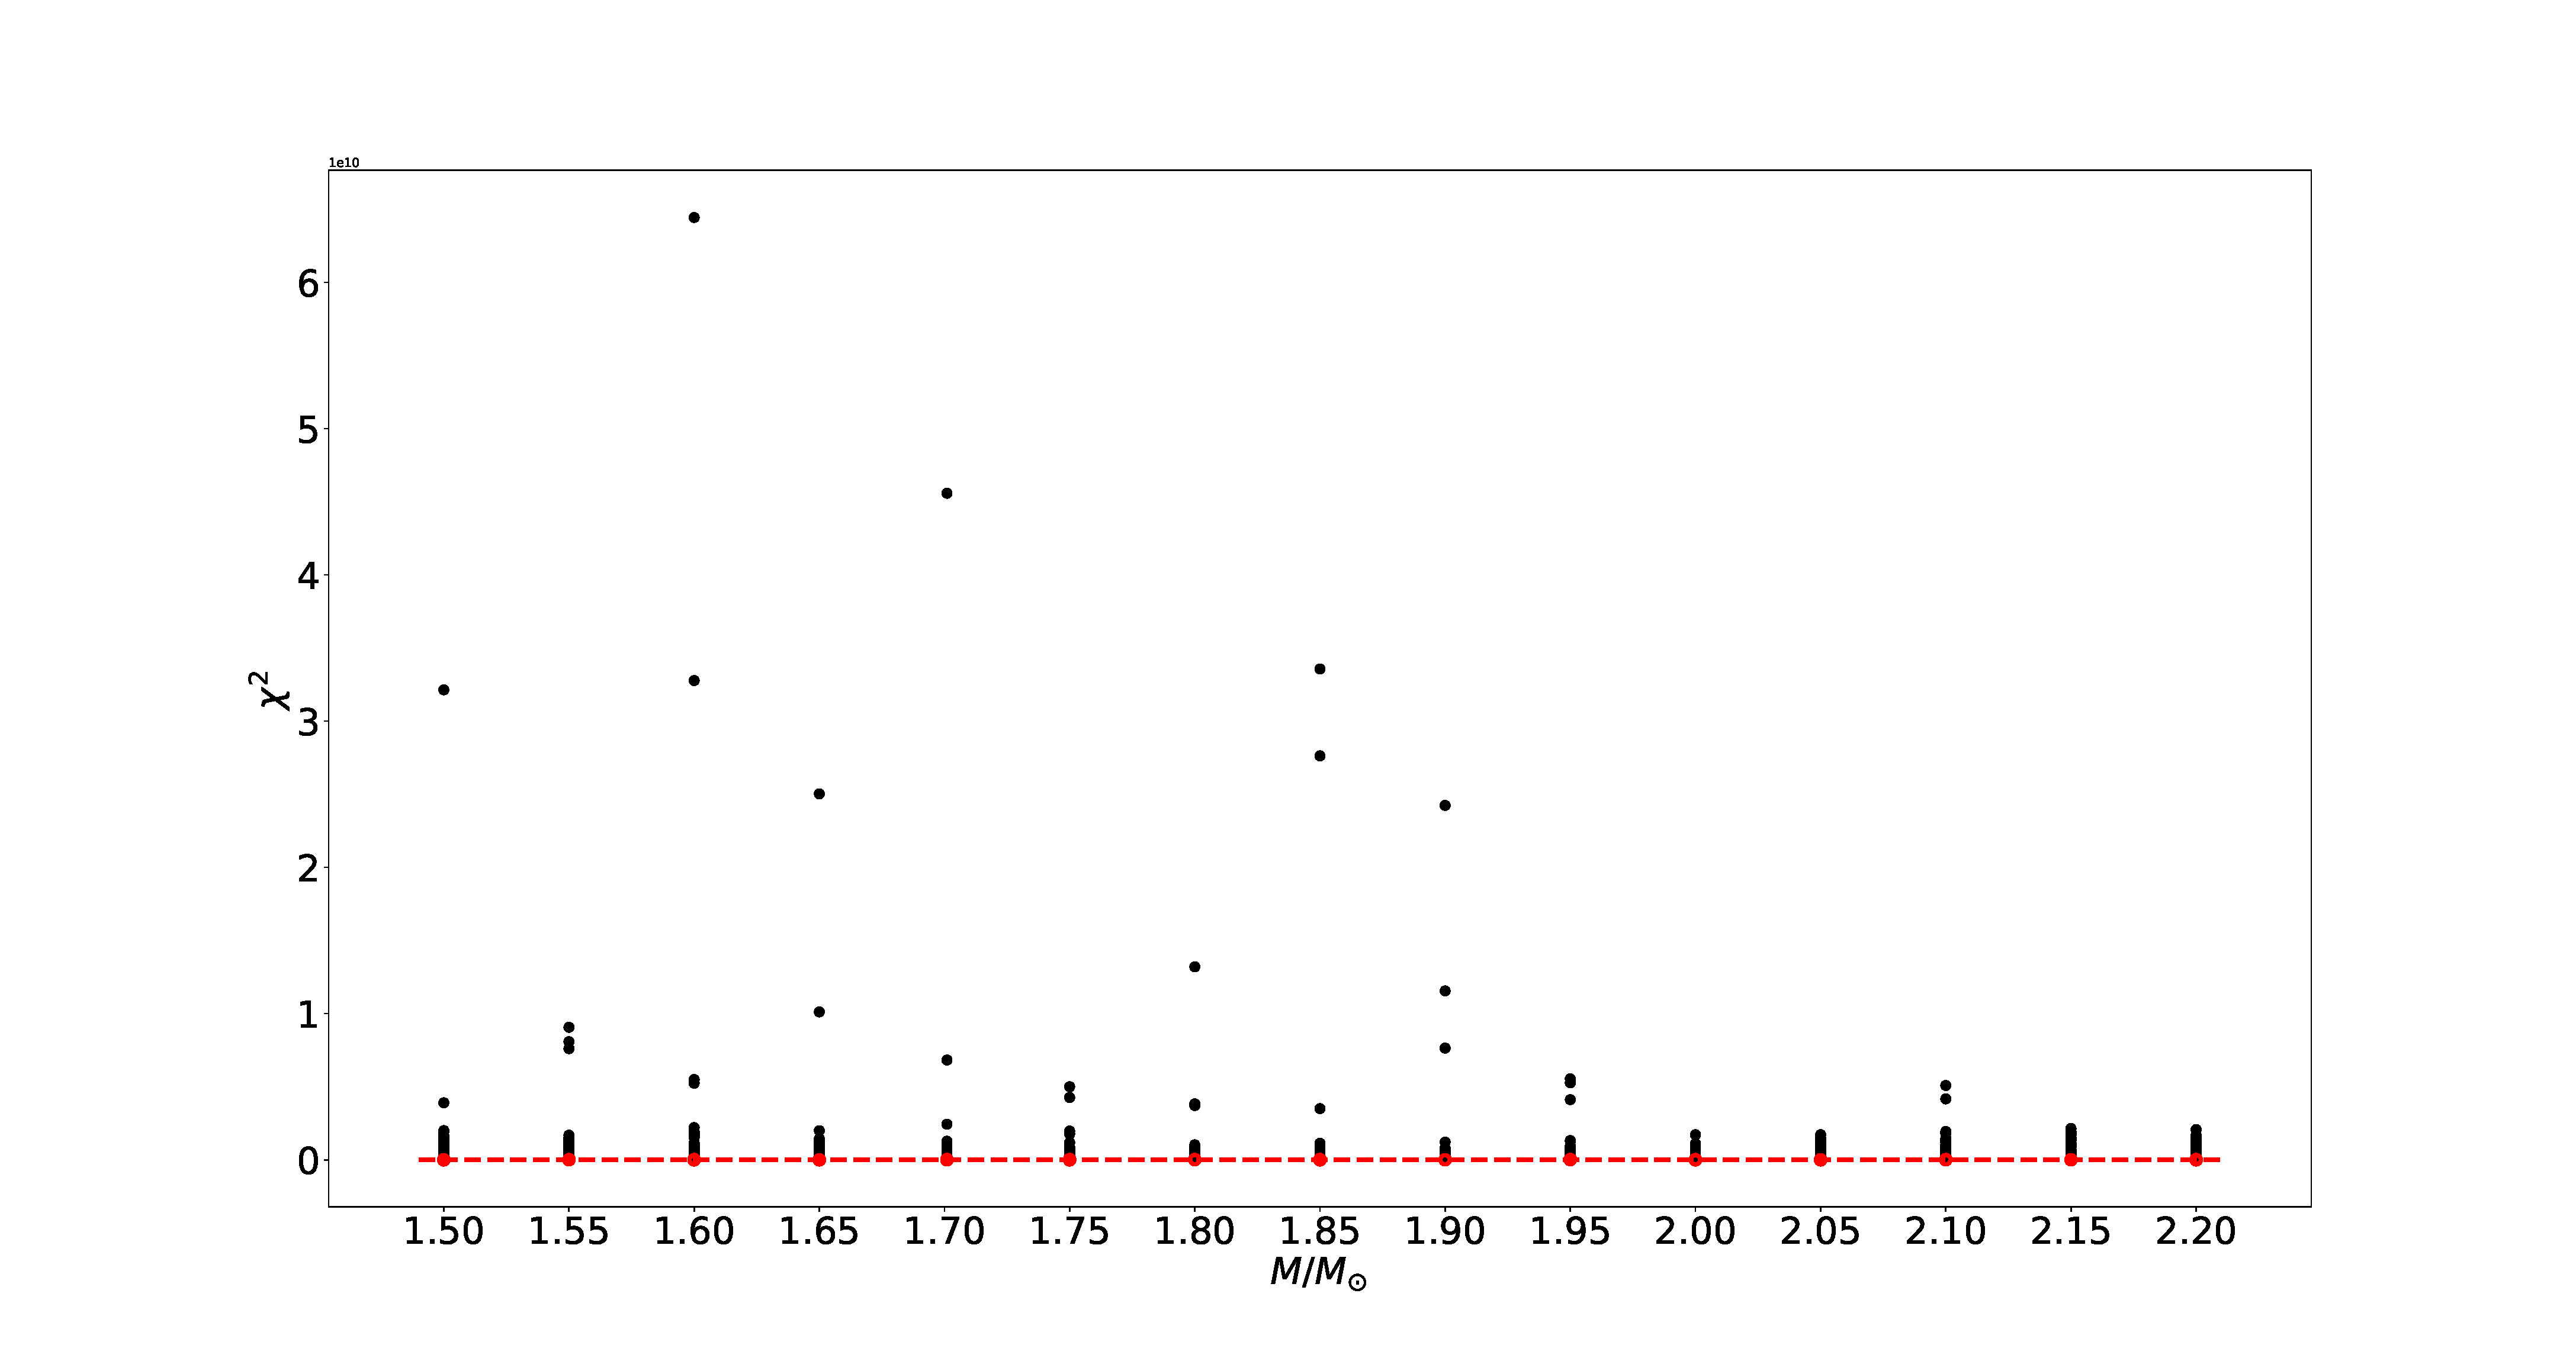
\includegraphics[width=1\textwidth]{appendix_stuff/plotchis.eps}
	\caption{Lowest \chis models for each track plotted as a function of mass. The red lines indicates the 5\% lower \chis limit for models to be included into the best 5\%.   }
	\label{selectfive}
\end{figure}

The non-radial pulsations are then calculated in \texttt{GYRE} for the 5\% best models. From these, the \chis routine for $l=0,1,2$ is run to obtain new \chis. This is done in \texttt{getl1l2\_results\_actually\_version2.py}

\lstinputlisting[language=python]{appendix_stuff/getl1l2_actually.py},

\noindent which produces the final output file. This file is then opened in \texttt{test\_l012\_results\_actually\_version2.py}.

\lstinputlisting[language=python]{appendix_stuff/test_l012_results_actually_version2.py},

 The output prints the minimum  $\chi_{tot}^2$,  $\chi_{obs}^2$, $\chi_{freqs}^2$  and $\chi_{p}^2$ (enhanced total \chis). All of these routines are for 44 Tau calculations. The routines for HD 187547 are similar, but with different directories. The \chis code also implements a routine for calculating the separation. This is done in \texttt{calculate\_chis\_ff1\_superstar\_withcorrectsep.py} called in the main file which is similar to the main file for 44 Tau, and is therefore not listed here).
 
\lstinputlisting[language=python]{appendix_stuff/calculate_chis_ff1_superstar_withcorrectsep.py}. 
 
 





%\section{The asteroseismic package}

% The astero module is an addition to the stellar evolution calculation tool MESA. It links to the two different stellar oscillation codes that calculate the stellar oscillation frequencies within MESA: ADIPLS and GYRE. It is specified within the ASTERO inlist files which should be used to create the oscillation frequencies. Even though these two packages serves the same purpose, their input physics are slighty different from each other. The ADIPLS package does not have non-adiabatic prescriptions, so for a $\delta$ Sct star the GYRE code is preferable. When the oscillation frequencies have been calculated, the ASTERO module implements algorithms to search for model parameters that best fit chosen observations. This gives an idea of how well the calculated frequencies reproduce observations.

% \subsection{Content}

% The ASTERO package consists of both log files, inlist files and executables and a mod file for the pre-main sequence model. The most relevant for this project being the inlist files, which are the files used to specify the parameters for 44 Tau. \texttt{Inlist\_3} is the relevant file regarding the MESA stellar evolution calculation. Here it is possible to specify the pre main-sequence model, opacities used, timestep, atmosphere prescription and plot specifics. For the asteroseismic part of the run, the inlist file used is \texttt{inlist\_astero\_search\_controls}. The input here should be the observables of 44 Tau, specifically $T_eff$, $log g$, $log L$, $[Fe/H]$ and the observed observation frequencies. It is possible to add more observables if they are known, but it should be kept in mind that the code can be slowed down significantly for every new input.

% It is also possible to specify the method to which the chi$^2$ terms are calculated, the most simple being \texttt{use\_first\_value}, meaning that calculation of stellar evolution and oscillation frequencies are based on start guesses. The variables that are guestimated are stellar Mass $M$, Helium abundance $Y_i$, metal abundance $Z_i$, mixing-length paramter $\alpha_{MLT}$ and finally the age of the star $T_{age}$. Using the first guesses for these variables a chi$^2$ fit is calculated for each variable seperately, and eventually the combination of parameters that results in the best chi$^2$ fit. The boundary conditions for the chi$^2$ fitting run can similarly be specified in the \texttt{inlist\_astero\_search\_controls}. 

% Besides from the inlist files, there are also a couple of executables. Before running the code, all files should be constructed by writing \texttt{./mk} in the linux terminal. This constructs all files needed for the code to run. This is done by typing $/.rn$. The code might take a long time depending on the input, which can be solved by making the timesteps larger. This does, however, correspond to calculating a larger chunk of the star in each step, which might not be favorable if the star is suspected to behave differently from others of the same type, or if it contains complicated processes. For instance it takes much longer to calculate the parameters for a very heavy star, as the processeses inside requries small timesteps to be resolved.

% When the code is has finished the run, the results are saved to different output files. The \texttt{LOGS} directory contains stellar parameters for all profiles calculated during the evolution run. All can be found in the \texttt{history} file, which can be used to create various plots including an HR-diagram. These are only result for the stellar evolution, but the ASTERO module also calculates and compares frequencies to observations by chi$^2$ fitting, and result for these can be found in the \texttt{outputs} directory. The file \texttt{sample\_0001.data} contains observed and calculated frequencies, chi$^2$ terms and estimated stellar parameters parameters that should reproduce the observed ones.  

% \subsection{44 Tau with ASTERO module}

% A run was made with parameters for 44 Tau. The start guesses and observables used in the inlist files can be seen in Table. What should be noticed is that only two frequencies are used in this inlist. The reason for this is that the ASTERO module is optimized for solar-like oscillators, which does not include $\delta$ Sct and therefore not 44 tau either. The input physics in the ASTERO module assumes that the star is a perfect sphere, meaning that non-radial oscillation frequencies are not reliable as input because rotation influences the symmetry and the spherical symmetry approximation becomes invalid. 





%\appendix
%\include{appendix}

\end{document}